% =============================================================================
% main.tex – Interaktives Auswahlpanel Dokumentation
% =============================================================================
% SSOT-Prinzip: Keine Redundanzen, alle Kapitel referenzieren SPEC
% Farbschema: Arduino Teal + Raspberry Pi Red + GitHub Dark
% Konsistent mit: praesentation.tex, schematic.css, cover-diagram.tex
% =============================================================================
\documentclass{techdoc}
% \documentclass[print]{techdoc}
% \documentclass[draft]{techdoc}

% =============================================================================
% METADATEN
% =============================================================================
\title{Interaktives Auswahlpanel}
\subtitle{100× Taster/LED + 100× Bild/MP3}
\tagline{„Drücken -- Leuchten -- Abspielen"}
\scope{ESP32S3 • Raspberry Pi 5 • Web-Dashboard}
\stack{CD4021BE \textbullet\ 74HC595 \textbullet\ PlatformIO \textbullet\ Python/aiohttp \textbullet\ WebSocket \textbullet\ HTML/JS \textbullet\ systemd}
\version{2.5.3}
\date{11.01.2026}
\author{Jan Unger}
\credits{Claude 4.5}
\coverimage{cover-selection-panel.pdf}

% Bilder liegen in ./images/ und ./covers/
\graphicspath{{images/}{covers/}}

\setheadertitle{Auswahlpanel}

\hypersetup{
  pdftitle={Interaktives Auswahlpanel},
  pdfsubject={100× Taster/LED + 100× Bild/MP3},
  pdfauthor={Jan Unger}
}

% =============================================================================
% PROJEKT-SPEZIFISCHE ERWEITERUNGEN
% =============================================================================

% Euro als SI-Einheit (für \SI{...}{\EUR} in Tabellen)
\DeclareSIUnit{\EUR}{\text{€}}

% Zusätzliche SI-Einheit
\DeclareSIUnit{\baud}{baud}

% Text-Macros (falls nicht in techdoc.cls)
\providecommand{\topic}[1]{\texttt{#1}}
\providecommand{\filep}[1]{\texttt{#1}}
\providecommand{\pin}[1]{\texttt{#1}}

% =============================================================================
% FARBDEFINITIONEN (falls nicht in techdoc.cls)
% =============================================================================

% Primärfarben
\definecolor{ArduinoTeal}{RGB}{0,151,157}
\definecolor{ArduinoDark}{RGB}{0,92,95}
\definecolor{RaspberryRed}{RGB}{197,26,74}
\definecolor{RaspberryPurple}{RGB}{117,38,74}

% Statusfarben
\definecolor{SuccessGreen}{RGB}{117,169,40}
\definecolor{WarningOrange}{RGB}{217,119,6}

% Hintergründe
\definecolor{GitHubDark}{RGB}{13,17,23}
\definecolor{SlateDark}{RGB}{30,41,51}
\definecolor{SlateMedium}{RGB}{45,58,69}

% Text
\definecolor{LightText}{RGB}{230,237,243}
\definecolor{MutedText}{RGB}{74,85,104}

% Signalfarben
\definecolor{SignalData}{RGB}{81,207,102}
\definecolor{SignalClock}{RGB}{255,212,59}
\definecolor{SignalLatch}{RGB}{77,171,247}

% Code-Farben
\definecolor{CodeBackground}{RGB}{248,250,252}
\definecolor{CodeFrame}{RGB}{200,210,220}
\definecolor{KeywordColor}{RGB}{0,92,95}
\definecolor{CommentColor}{RGB}{74,85,104}
\definecolor{StringColor}{RGB}{197,26,74}

% Info-Box-Farben
\definecolor{InfoBoxBg}{RGB}{230,245,250}
\definecolor{InfoBoxFrame}{RGB}{0,151,157}
\definecolor{WarnBoxBg}{RGB}{255,247,237}
\definecolor{WarnBoxFrame}{RGB}{217,119,6}
\definecolor{TipBoxBg}{RGB}{240,250,240}
\definecolor{TipBoxFrame}{RGB}{117,169,40}

% TikZ-Style für Abwärtskompatibilität (ROADMAP.tex)
\tikzset{
  CurrentBlue/.style={text=ArduinoTeal}
}

% Farb-Aliase für Abwärtskompatibilität
\colorlet{MainColor}{ArduinoTeal}
\colorlet{MainColorDark}{ArduinoDark}
\colorlet{AccentColor}{RaspberryRed}
\colorlet{DarkGray}{GitHubDark}
\colorlet{CurrentBlue}{ArduinoTeal}
\colorlet{arduinoblue}{ArduinoTeal}
\colorlet{codebg}{CodeBackground}
\colorlet{codeframe}{CodeFrame}
\colorlet{keywordcolor}{KeywordColor}
\colorlet{commentcolor}{CommentColor}
\colorlet{stringcolor}{StringColor}
\colorlet{infoboxbg}{InfoBoxBg}
\colorlet{infoboxframe}{InfoBoxFrame}
\colorlet{warnbg}{WarnBoxBg}
\colorlet{warnframe}{WarnBoxFrame}
\colorlet{tipbg}{TipBoxBg}
\colorlet{tipframe}{TipBoxFrame}

% Highlight-Befehle
\providecommand{\highlight}[1]{\textcolor{ArduinoTeal}{\textbf{#1}}}
\providecommand{\improvement}[1]{\textcolor{SuccessGreen}{\textbf{#1}}}
\providecommand{\warning}[1]{\textcolor{WarningOrange}{\textbf{#1}}}
\providecommand{\critical}[1]{\textcolor{RaspberryRed}{\textbf{#1}}}

% JavaScript Listing-Style (falls nicht in techdoc.cls)
\lstdefinestyle{javascript}{
  language=Java,
  basicstyle=\ttfamily\small,
  keywordstyle=\color{KeywordColor}\bfseries,
  commentstyle=\color{CommentColor}\itshape,
  stringstyle=\color{StringColor},
  numbers=left, numberstyle=\tiny\color{MutedText},
  frame=single, framesep=4pt, rulecolor=\color{CodeFrame},
  backgroundcolor=\color{CodeBackground},
  breaklines=true, breakatwhitespace=true, showstringspaces=false,
  tabsize=2, captionpos=b,
  xleftmargin=12pt, xrightmargin=4pt, aboveskip=1.2em, belowskip=1.2em,
  morekeywords={const,let,async,await,function,return,if,else,for,while,
                true,false,null,undefined,this,new,class,export,import,
                document,window,console,fetch,Promise,setTimeout,
                addEventListener,getElementById,querySelector}
}

% =============================================================================
% DOKUMENT
% =============================================================================
\begin{document}

\maketitlepage

\pagenumbering{roman}
\tableofcontents
\clearpage
\pagenumbering{arabic}

% =============================================================================
% INHALT – Modulare Struktur (SSOT)
% =============================================================================

% --- Setup & Voraussetzungen ---
% =============================================================================
% VORAUSSETZUNGEN.tex – Hardware & Software für das Selection-Panel
% Modulares Fragment (kein \documentclass, kein \begin{document})
% Stand: 2026-01-08 | Version: 2.5.2
% =============================================================================

\section{Voraussetzungen}
\label{sec:voraussetzungen}

Bevor wir mit dem Aufbau beginnen, werfen wir einen Blick auf die benötigte Hardware und Software. Die folgende Übersicht zeigt alle Komponenten, die wir für das Selection-Panel-Projekt benötigen.

% -----------------------------------------------------------------------------
\subsection{Hardware}
\label{subsec:voraussetzungen-hardware}

\Cref{tab:hardware-komponenten} listet die Kernkomponenten auf. Bei der Auswahl haben wir auf ein ausgewogenes Verhältnis zwischen Leistung und Kosten geachtet.

\begin{table}[H]
  \centering
  \caption{Hardware-Komponenten für das Selection-Panel}
  \label{tab:hardware-komponenten}
  \begin{tabularx}{\textwidth}{@{}l X l r@{}}
    \toprule
    \textbf{Komponente} & \textbf{Zweck} & \textbf{Bezugsquelle} & \textbf{Preis} \\
    \midrule
    Raspberry Pi 5, \SI{4}{\giga\byte} RAM & Server, Media-Ausgabe & BerryBase (RPI5-4GB) & \SI{71,50}{\EUR} \\
    Raspberry Pi Active Cooler & Kühlung & BerryBase (RPI5-ACOOL) & \SI{5,90}{\EUR} \\
    Raspberry Pi \SI{27}{\watt} USB-C Netzteil & Stromversorgung & BerryBase (RPI5NT5AW) & \SI{12,40}{\EUR} \\
    SanDisk Extreme microSDXC \SI{128}{\giga\byte} & Betriebssystem & BerryBase (A2 UHS-I U3 V30) & $\sim$\SI{18}{\EUR} \\
    HDMI Adapter Micro-D → A & Monitor & BerryBase (8007067) & \SI{1,10}{\EUR} \\
    Seeed XIAO ESP32-S3 & Taster/LEDs & Reichelt & $\sim$\SI{9}{\EUR} \\
    \bottomrule
  \end{tabularx}
\end{table}

\begin{tipbox}[Bezugsquelle]
  Alle Raspberry-Pi-Komponenten sind bei \href{https://www.berrybase.de}{BerryBase.de} erhältlich. Preise Stand Januar 2026.
\end{tipbox}

% -----------------------------------------------------------------------------
\subsection{Software (Entwicklungsrechner)}
\label{subsec:voraussetzungen-software}

Je nach Betriebssystem unterscheidet sich die Installation der Entwicklungswerkzeuge. Wir zeigen hier die Schritte für macOS, Windows und Linux.

\subsubsection{macOS}

Unter macOS nutzen wir Homebrew als Paketmanager:

\begin{lstlisting}[style=shell]
/bin/bash -c "$(curl -fsSL https://raw.githubusercontent.com/Homebrew/install/HEAD/install.sh)"
brew install python git vim
\end{lstlisting}

\subsubsection{Windows}

Unter Windows installieren wir die Tools manuell:

\begin{enumerate}
  \item \textbf{Git:} Download von \href{https://git-scm.com/download/win}{git-scm.com/download/win}
  \item \textbf{Python:} Download von \href{https://www.python.org/downloads/}{python.org/downloads} – Option \enquote{Add Python to PATH} aktivieren
\end{enumerate}

\subsubsection{Linux (Ubuntu/Debian)}

Unter Linux greifen wir auf die Paketverwaltung zurück:

\begin{lstlisting}[style=shell]
sudo apt update && sudo apt install python3 python3-pip python3-venv git vim
\end{lstlisting}

% -----------------------------------------------------------------------------
\subsection{VS Code + PlatformIO}
\label{subsec:voraussetzungen-platformio}

Für die Firmware-Entwicklung setzen wir auf VS Code mit der PlatformIO-Extension:

\begin{enumerate}
  \item \textbf{VS Code} von \href{https://code.visualstudio.com/}{code.visualstudio.com} herunterladen und installieren
  \item Die Extension \texttt{PlatformIO IDE} über den Marketplace installieren
\end{enumerate}

\Cref{tab:platformio-befehle} fasst die wichtigsten PlatformIO-Befehle zusammen. Mit diesen vier Kommandos decken wir den gesamten Entwicklungszyklus ab.

\begin{table}[H]
  \centering
  \caption{PlatformIO-Befehle für die ESP32-Entwicklung}
  \label{tab:platformio-befehle}
  \begin{tabularx}{\textwidth}{@{}l X@{}}
    \toprule
    \textbf{Aktion} & \textbf{Befehl} \\
    \midrule
    Kompilieren & \texttt{pio run} \\
    Flashen & \texttt{pio run -t upload} \\
    Serial-Monitor & \texttt{pio device monitor} \\
    Flash + Monitor & \texttt{pio run -t upload -t monitor} \\
    \bottomrule
  \end{tabularx}
\end{table}

% -----------------------------------------------------------------------------
\subsection{Referenz-System}
\label{subsec:voraussetzungen-referenz}

Die folgende Konfiguration dient als Referenz für die Dokumentation. Wenn wir auf Versionsnummern oder Verhaltensweisen verweisen, beziehen wir uns auf dieses Setup.

\begin{table}[H]
  \centering
  \caption{Hardware-Referenz}
  \label{tab:referenz-hardware}
  \begin{tabularx}{0.7\textwidth}{@{}l X@{}}
    \toprule
    \textbf{Hardware} & \textbf{Version} \\
    \midrule
    Board & Raspberry Pi 5 Model B Rev 1.1 \\
    Microcontroller & Seeed XIAO ESP32-S3 \\
    \bottomrule
  \end{tabularx}
\end{table}

\begin{table}[H]
  \centering
  \caption{Software-Versionen}
  \label{tab:referenz-software}
  \begin{tabularx}{0.7\textwidth}{@{}l X@{}}
    \toprule
    \textbf{Software} & \textbf{Version} \\
    \midrule
    Pi OS & Debian 13 (trixie), Build 2025-12-04 \\
    Python & 3.13+ \\
    aiohttp & 3.9+ \\
    PlatformIO & 6.x \\
    Firmware & 2.5.2 \\
    Server & 2.5.2 \\
    Dashboard & 2.5.1 \\
    \bottomrule
  \end{tabularx}
\end{table}

% -----------------------------------------------------------------------------
\subsection{Checkliste}
\label{subsec:voraussetzungen-checkliste}

Bevor wir zum nächsten Kapitel übergehen, prüfen wir kurz, ob alle Voraussetzungen erfüllt sind.

\subsubsection{Hardware}

\begin{itemize}
  \item[$\square$] Raspberry Pi 5 + Active Cooler
  \item[$\square$] microSD-Karte (\SI{128}{\giga\byte})
  \item[$\square$] ESP32-S3 XIAO
  \item[$\square$] USB-C Kabel (Daten, nicht nur Laden)
  \item[$\square$] Multimeter
\end{itemize}

\subsubsection{Software}

\begin{itemize}
  \item[$\square$] Git: \texttt{git --version}
  \item[$\square$] Python: \texttt{python3 --version}
  \item[$\square$] VS Code + PlatformIO
  \item[$\square$] SSH-Zugang zum Pi
\end{itemize}

\begin{warnbox}[USB-Kabel beachten]
  Viele USB-C-Kabel übertragen nur Strom, keine Daten. Ein defektes oder reines Ladekabel ist eine häufige Fehlerquelle beim Flashen des ESP32.
\end{warnbox}

% -----------------------------------------------------------------------------
\subsection{Nächste Schritte}
\label{subsec:voraussetzungen-naechste}

Mit der Hardware auf dem Tisch und der installierten Software können wir nun in die praktische Umsetzung einsteigen. \Cref{tab:naechste-schritte} zeigt den empfohlenen Ablauf.

\begin{table}[H]
  \centering
  \caption{Weiterführende Dokumentation}
  \label{tab:naechste-schritte}
  \begin{tabularx}{\textwidth}{@{}l X@{}}
    \toprule
    \textbf{Schritt} & \textbf{Dokument} \\
    \midrule
    Pi einrichten + SSH & → \Cref{sec:ssh} \\
    Repository klonen & → \Cref{sec:git} \\
    Server starten & → \Cref{sec:quickstart} \\
    Löten & → \Cref{sec:loeten} \\
    \bottomrule
  \end{tabularx}
\end{table}

% =============================================================================
% SSH.tex – Pi einrichten und passwortloses SSH konfigurieren
% Modulares Fragment (kein \documentclass, kein \begin{document})
% Stand: 2026-01-08 | Version: 2.5.2
% =============================================================================

\section{SSH-Setup}
\label{sec:ssh}

Bevor wir mit der Entwicklung beginnen können, richten wir den Raspberry Pi ein und konfigurieren einen passwortlosen SSH-Zugang. Das Ziel: Mit einem simplen \texttt{ssh rover} landen wir direkt auf dem Pi – ohne Passwortabfrage.

% -----------------------------------------------------------------------------
\subsection{Pi OS installieren}
\label{subsec:ssh-pi-os}

Wir nutzen den offiziellen Raspberry Pi Imager, um das Betriebssystem auf die SD-Karte zu schreiben.

\subsubsection{Raspberry Pi Imager}

\begin{enumerate}
  \item \textbf{Download:} \href{https://www.raspberrypi.com/software/}{raspberrypi.com/software}
  \item \textbf{OS auswählen:} Raspberry Pi OS Lite (64-bit)
  \item \textbf{Einstellungen} über das Zahnrad-Symbol konfigurieren (\cref{tab:imager-settings})
  \item \textbf{Schreiben} – SD-Karte einlegen – Netzteil einstecken
\end{enumerate}

\begin{table}[H]
  \centering
  \caption{Einstellungen im Raspberry Pi Imager}
  \label{tab:imager-settings}
  \begin{tabularx}{0.7\textwidth}{@{}l X@{}}
    \toprule
    \textbf{Einstellung} & \textbf{Wert} \\
    \midrule
    Hostname & \texttt{rover} \\
    SSH & ✓ aktivieren \\
    Benutzer & \texttt{pi} \\
    Passwort & (eigenes Passwort) \\
    WLAN & SSID + Passwort \\
    Zeitzone & \texttt{Europe/Berlin} \\
    \bottomrule
  \end{tabularx}
\end{table}

\subsubsection{Nach dem ersten Boot}

Sobald der Pi hochgefahren ist, verbinden wir uns erstmals per SSH und führen die Grundkonfiguration durch:

\begin{lstlisting}[style=shell]
ssh pi@rover.local
sudo apt update && sudo apt upgrade -y
sudo usermod -aG dialout pi
\end{lstlisting}

Der letzte Befehl fügt den Benutzer \texttt{pi} zur Gruppe \texttt{dialout} hinzu – das benötigen wir später für den Zugriff auf den ESP32 über USB.

% -----------------------------------------------------------------------------
\subsection{SSH-Key einrichten}
\label{subsec:ssh-key}

Passwörter sind umständlich und unsicher. Wir generieren stattdessen ein Schlüsselpaar und kopieren den öffentlichen Schlüssel auf den Pi.

\subsubsection{Mac / Linux}

\begin{lstlisting}[style=shell]
ssh-keygen -t ed25519
ssh-copy-id pi@rover.local
\end{lstlisting}

Der erste Befehl erzeugt ein Ed25519-Schlüsselpaar (aktueller Standard, kompakt und sicher). Der zweite kopiert den Public Key automatisch in die \filep{authorized\_keys} des Pi.

\subsubsection{Windows (PowerShell)}

Unter Windows müssen wir zunächst den OpenSSH-Client aktivieren:

\begin{lstlisting}[style=shell,language={}]
# OpenSSH aktivieren (als Admin ausfuehren)
Add-WindowsCapability -Online -Name OpenSSH.Client~~~~0.0.1.0

# Key erstellen
ssh-keygen -t ed25519

# Key manuell kopieren
type $env:USERPROFILE\.ssh\id_ed25519.pub |
ssh pi@rover.local "mkdir -p ~/.ssh && cat >> ~/.ssh/authorized_keys && chmod 600 ~/.ssh/authorized_keys"
\end{lstlisting}

\begin{infobox}[Warum Ed25519?]
  Ed25519 bietet bei nur \SI{256}{\bit} Schlüssellänge eine Sicherheit vergleichbar mit RSA-3072. Die Schlüssel sind kompakter und die Signaturoperationen schneller.
\end{infobox}

% -----------------------------------------------------------------------------
\subsection{SSH-Config anlegen}
\label{subsec:ssh-config}

Mit einer SSH-Konfigurationsdatei sparen wir uns künftig die Tipparbeit. Statt \texttt{ssh pi@rover.local} genügt dann \texttt{ssh rover}.

\subsubsection{Mac / Linux}

Wir erstellen oder erweitern die Datei \filep{\textasciitilde/.ssh/config}:

\begin{lstlisting}[style=shell,numbers=none]
Host rover
    HostName rover.local
    User pi
    IdentityFile ~/.ssh/id_ed25519
\end{lstlisting}

Die Berechtigungen müssen stimmen:

\begin{lstlisting}[style=shell]
chmod 600 ~/.ssh/config
\end{lstlisting}

\subsubsection{Windows}

Die Config-Datei liegt unter \filep{\%USERPROFILE\%\textbackslash.ssh\textbackslash config}:

\begin{lstlisting}[style=shell,numbers=none]
Host rover
    HostName rover.local
    User pi
    IdentityFile ~/.ssh/id_ed25519
\end{lstlisting}

\begin{tipbox}[Verbindung testen]
  Nach der Konfiguration testen wir mit \texttt{ssh rover}. Wenn alles funktioniert, landen wir ohne Passwortabfrage direkt auf dem Pi.
\end{tipbox}

% -----------------------------------------------------------------------------
\subsection{GitHub-Zugang einrichten}
\label{subsec:ssh-github}

Für den Zugriff auf GitHub-Repositories erstellen wir einen separaten Schlüssel:

\begin{lstlisting}[style=shell]
ssh-keygen -t ed25519 -f ~/.ssh/id_ed25519_github
\end{lstlisting}

Die SSH-Config erweitern wir um einen Eintrag für GitHub:

\begin{lstlisting}[style=shell,numbers=none]
Host github.com
    HostName github.com
    User git
    IdentityFile ~/.ssh/id_ed25519_github
    IdentitiesOnly yes
\end{lstlisting}

Den Public Key hinterlegen wir bei GitHub unter \textit{Settings → SSH Keys → New SSH Key}. Den Inhalt der Datei \filep{\textasciitilde/.ssh/id\_ed25519\_github.pub} kopieren wir in das Textfeld.

\begin{lstlisting}[style=shell]
# Verbindung testen
ssh -T git@github.com
# Erwartete Ausgabe: "Hi username! You've successfully authenticated..."
\end{lstlisting}

% -----------------------------------------------------------------------------
\subsection{Serial-Port-Berechtigungen}
\label{subsec:ssh-serial}

Damit wir den ESP32 über USB ansprechen können, benötigt der Benutzer \texttt{pi} Zugriff auf die Serial-Ports:

\begin{lstlisting}[style=shell]
# Auf dem Pi ausfuehren
sudo usermod -aG dialout pi
# Danach neu einloggen (oder reboot)

# Stabilen by-id Pfad pruefen
ls -la /dev/serial/by-id/usb-Espressif*
\end{lstlisting}

\begin{warnbox}[Neu einloggen erforderlich]
  Gruppenmitgliedschaften werden erst nach einem neuen Login aktiv. Ein einfaches \texttt{exit} und erneutes \texttt{ssh rover} genügt.
\end{warnbox}

% -----------------------------------------------------------------------------
\subsection{Troubleshooting}
\label{subsec:ssh-troubleshooting}

\Cref{tab:ssh-troubleshooting} listet die häufigsten Probleme und deren Lösungen.

\begin{table}[H]
  \centering
  \caption{SSH-Fehlerbehebung}
  \label{tab:ssh-troubleshooting}
  \begin{tabularx}{\textwidth}{@{}l X@{}}
    \toprule
    \textbf{Problem} & \textbf{Lösung} \\
    \midrule
    \texttt{Permission denied (publickey)} & \texttt{ssh-copy-id} erneut ausführen \\
    \texttt{Could not resolve hostname} & IP direkt nutzen: \texttt{ssh pi@192.168.x.x} \\
    \texttt{UNPROTECTED PRIVATE KEY FILE} & Berechtigungen setzen: \texttt{chmod 600 \textasciitilde/.ssh/id\_ed25519} \\
    Serial-Port nicht zugänglich & Gruppe hinzufügen: \texttt{sudo usermod -aG dialout pi} \\
    mDNS funktioniert nicht & Avahi prüfen: \texttt{sudo systemctl status avahi-daemon} \\
    \bottomrule
  \end{tabularx}
\end{table}

\begin{infobox}[IP-Adresse ermitteln]
  Falls \texttt{rover.local} nicht auflöst, finden wir die IP über den Router oder – falls wir noch einen Monitor am Pi haben – mit \texttt{hostname -I}.
\end{infobox}


% --- Hardware ---
% =============================================================================
% HARDWARE.tex – Selection Panel Hardware
% =============================================================================
% Einbindung: % =============================================================================
% HARDWARE.tex – Selection Panel Hardware
% =============================================================================
% Einbindung: % =============================================================================
% HARDWARE.tex – Selection Panel Hardware
% =============================================================================
% Einbindung: \input{content/HARDWARE.tex}
% Version: 2.5.2 | Stand: 2026-01-11
% =============================================================================

\section{Hardware}
\label{sec:hardware}

Dieses Kapitel dokumentiert den 10-Button-Prototyp des Selection Panels. Die Schaltung
lässt sich auf 100 Taster skalieren, indem wir die Daisy-Chain der Schieberegister
verlängern.

% -----------------------------------------------------------------------------
\subsection{Komponentenübersicht}
\label{subsec:hw-komponenten}

\begin{table}[H]
\centering
\caption{Stückliste des 10-Button-Prototyps}
\label{tab:hw-komponenten}
\begin{tabularx}{\textwidth}{@{}l l r X@{}}
\toprule
\textbf{Komponente} & \textbf{Typ} & \textbf{Anzahl} & \textbf{Funktion} \\
\midrule
XIAO ESP32-S3       & Mikrocontroller         & 1  & Steuerlogik, USB-CDC \\
Raspberry Pi 5      & SBC + Netzteil + microSD & 1 & Server, Dashboard, Medien \\
CD4021B             & 8-Bit PISO Schieberegister & 2 & Taster einlesen \\
74HC595             & 8-Bit SIPO Schieberegister & 2 & LEDs ansteuern \\
Taster              & $6 \times 6$\,\si{\milli\meter} Tactile Switch & 10 & Benutzereingabe \\
LED                 & \SI{5}{\milli\meter}, versch.\ Farben & 10 & Statusanzeige \\
Widerstand          & \SIrange{330}{3000}{\ohm} & 10 & LED-Strombegrenzung \\
Widerstand          & \SI{10}{\kilo\ohm}       & 10 & Pull-up für Taster \\
Kondensator         & \SI{100}{\nano\farad} (Keramik) & 4 & Stützkondensatoren \\
\bottomrule
\end{tabularx}
\end{table}

% -----------------------------------------------------------------------------
\subsection{Pin-Belegung XIAO ESP32-S3}
\label{subsec:hw-pinout}

\begin{figure}[H]
\centering
\begin{lstlisting}[basicstyle=\ttfamily\footnotesize, frame=single, numbers=none]
                  +-------------+
                  |    USB-C    |
                  |             |
 LED_RCK    D0 ---|  1       14 |--- 5V
 BTN_PS     D1 ---|  2       13 |--- GND
 LED_OE     D2 ---|  3       12 |--- 3V3
            D3 ---|  4       11 |--- D10  LED_MOSI
            D4 ---|  5       10 |--- D9   BTN_MISO
            D5 ---|  6        9 |--- D8   SCK
            D6 ---|  7        8 |--- D7
                  |             |
                  +-------------+
\end{lstlisting}
\caption{Pin-Belegung des XIAO ESP32-S3}
\label{fig:xiao-pinout}
\end{figure}

\begin{table}[H]
\centering
\caption{GPIO-Zuordnung für SPI und Steuerung}
\label{tab:gpio-zuordnung}
\begin{tabularx}{\textwidth}{@{}l l l X@{}}
\toprule
\textbf{Pin} & \textbf{Signal} & \textbf{Funktion} & \textbf{Ziel} \\
\midrule
\pin{D0}  & \texttt{LED\_RCK}  & Latch (STCP)              & 74HC595 Pin 12 \\
\pin{D1}  & \texttt{BTN\_PS}   & Parallel/Serial Control   & CD4021B Pin 9 \\
\pin{D2}  & \texttt{LED\_OE}   & Output Enable (PWM, active-low) & 74HC595 Pin 13 \\
\pin{D8}  & \texttt{SCK}       & SPI Clock                 & Beide Chip-Typen \\
\pin{D9}  & \texttt{BTN\_MISO} & Daten von CD4021B         & CD4021B \#0 Pin 3 (Q8) \\
\pin{D10} & \texttt{LED\_MOSI} & Daten zu 74HC595          & 74HC595 \#0 Pin 14 (SER) \\
\bottomrule
\end{tabularx}
\end{table}

% -----------------------------------------------------------------------------
\subsection{Byte-Mapping (Firmware \texorpdfstring{$\leftrightarrow$}{<->} Hardware)}
\label{subsec:hw-byte-mapping}

Die Asymmetrie zwischen Ein- und Ausgabe ergibt sich aus der Hardware: Der CD4021B
schiebt sein erstes Sample (PI-8) als erstes Bit heraus, während der 74HC595 das
zuletzt empfangene Bit auf QA (Ausgang 0) legt.

\begin{table}[H]
\centering
\caption{Bit-Zuordnung der Schieberegister}
\label{tab:byte-mapping}
\begin{tabular}{@{}l l l@{}}
\toprule
\textbf{IC} & \textbf{Byte 0} & \textbf{Byte 1} \\
\midrule
74HC595 (LEDs)    & LED 1--8 = Bit 0--7 & LED 9--10 = Bit 0--1 \\
CD4021 (Taster)   & BTN 1--8 = Bit 7--0 & BTN 9--10 = Bit 7--6 \\
\bottomrule
\end{tabular}
\end{table}

\begin{infobox}[Firmware-Abstraktion]
Die Firmware verwendet in \filep{bitops.h} die Formel \lstinline[style=arduino]|btn_bit(id) = 7 - ((id - 1) % 8)|,
um diese Zuordnung zu abstrahieren. Damit arbeitet die Logik-Schicht einheitlich mit
Button-IDs von 1--100.
\end{infobox}

% -----------------------------------------------------------------------------
\subsection{Schaltplan-Übersicht}
\label{subsec:hw-schaltplan}

\begin{figure}[H]
\centering
\begin{lstlisting}[basicstyle=\ttfamily\scriptsize, frame=single, numbers=none]
                        +--------------------------------------------------+
                        |                  OUTPUT (LEDs)                   |
    +---------+         |                                                  |
    | Pi 5    |         |   +----------+  QH'     +----------+             |
    |         |  USB-C  |   | 74HC595  |--------->| 74HC595  |             |
    |         |<------->|   |   #0     |   SER    |   #1     |             |
    +---------+         |   |          |          |          |             |
                        |   | QA-QH    |          | QA-QB    |             |
        +---------+     |   |   |      |          |   |      |             |
        |  XIAO   |     |   | LED 1-8  |          | LED 9-10 |             |
        | ESP32S3 |     |   +----------+          +----------+             |
        |         |     +--------------------------------------------------+
        | D10 ----+----------> SER #0 (MOSI)
        | D8  ----+----------> SCK (beide)
        | D0  ----+----------> RCK (beide)
        | D2  ----+----------> OE (beide)
        |         |
        | D9  <---+---------- Q8 #0 (MISO)
        | D8  ----+----------> CLK (beide)
        | D1  ----+----------> P/S (beide)
        |         |     +--------------------------------------------------+
        +---------+     |                  INPUT (Taster)                  |
                        |                                                  |
                        |   +----------+          +----------+             |
                        |   | CD4021B  |<-- DS ---| CD4021B  |<-- DS -- 3V3|
                        |   |   #0     |    Q8    |   #1     |             |
                        |   |          |<---------|          |             |
                        |   | PI 8-1   |          | PI 8-7   |             |
                        |   |   |      |          |   |      |             |
                        |   | BTN 1-8  |          | BTN 9-10 |             |
                        |   +----------+          +----------+             |
                        |        |                                         |
                        |        v                                         |
                        |      Q8 --> D9 (MISO)                            |
                        +--------------------------------------------------+
\end{lstlisting}
\caption{Gesamtübersicht der Schaltung}
\label{fig:schaltplan-uebersicht}
\end{figure}

% -----------------------------------------------------------------------------
\subsection{74HC595 Detailschaltplan (LED-Ausgang)}
\label{subsec:hw-74hc595}

Der 74HC595 ist ein Serial-In/Parallel-Out Schieberegister mit Latch. Die Daten
werden seriell eingetaktet und erst beim Latch-Impuls (RCK) an die Ausgänge
übernommen.

\begin{figure}[H]
\centering
\begin{lstlisting}[basicstyle=\ttfamily\scriptsize, frame=single, numbers=none]
                     74HC595 (#0)                    74HC595 (#1)
                  +-------------+                 +-------------+
    LED 2  <------|  1 QB  VCC 16|--- 3V3 LED 10 <|  1 QB  VCC 16|--- 3V3
    LED 3  <------|  2 QC  QA  15|--> LED 1       |  2 QC  QA  15|--> LED 9
    LED 4  <------|  3 QD  SER 14|<-- D10 (MOSI)  |  3 QD  SER 14|<-- #0.QH'
    LED 5  <------|  4 QE  OE  13|<-- D2 (PWM)    |  4 QE  OE  13|<-- D2 (PWM)
    LED 6  <------|  5 QF  RCK 12|<-- D0 (RCK)    |  5 QF  RCK 12|<-- D0 (RCK)
    LED 7  <------|  6 QG  SCK 11|<-- D8 (SCK)    |  6 QG  SCK 11|<-- D8 (SCK)
    LED 8  <------|  7 QH  CLR 10|--- 3V3         |  7 QH  CLR 10|--- 3V3
          GND ----|  8 GND QH'  9|---> #1.SER     |  8 GND QH'  9|    (n.c.)
                  +------+------+                 +------+------+
                         |                               |
                        === C1                          === C2
                        100nF                           100nF
                         |                               |
                        GND                             GND
\end{lstlisting}
\caption{74HC595 Pinout und Daisy-Chain}
\label{fig:74hc595-detail}
\end{figure}

\begin{warnbox}[CLR-Pin nicht floaten!]
Der \pin{CLR}-Pin (Pin 10) muss auf \SI{3.3}{\volt} gelegt werden. Ein floatender
CLR-Pin führt zu sporadischem Löschen des Schieberegisters.
\end{warnbox}

\subsubsection{LED-Beschaltung (Active-High)}

\begin{figure}[H]
\centering
\begin{lstlisting}[basicstyle=\ttfamily\small, frame=single, numbers=none]
    Qx (74HC595)
     |
    +-+
    | | 330 - 3k Ohm
    +-+
     |
     v LED
     |
    GND
\end{lstlisting}
\caption{LED-Vorwiderstand-Beschaltung}
\label{fig:led-beschaltung}
\end{figure}

Die Stromberechnung für verschiedene Widerstandswerte bei einer LED-Flussspannung
von ca.\ \SI{2.0}{\volt}:

\begin{table}[H]
\centering
\caption{LED-Strom in Abhängigkeit vom Vorwiderstand}
\label{tab:led-strom}
\begin{tabular}{@{}r r l@{}}
\toprule
\textbf{Widerstand} & \textbf{Strom} & \textbf{Helligkeit} \\
\midrule
\SI{330}{\ohm}  & $\approx$\,\SI{4}{\milli\ampere}   & hell \\
\SI{1}{\kilo\ohm}   & $\approx$\,\SI{1.3}{\milli\ampere} & gedimmt \\
\SI{3}{\kilo\ohm}   & $\approx$\,\SI{0.4}{\milli\ampere} & schwach \\
\bottomrule
\end{tabular}
\end{table}

% -----------------------------------------------------------------------------
\subsection{CD4021B Detailschaltplan (Taster-Eingang)}
\label{subsec:hw-cd4021b}

Der CD4021B ist ein Parallel-In/Serial-Out Schieberegister. Er liest acht
parallele Eingänge ein und gibt sie seriell aus.

\subsubsection{Pinout}

\begin{figure}[H]
\centering
\begin{lstlisting}[basicstyle=\ttfamily\small, frame=single, numbers=none]
              +------------+
    PI-8  ----|  1  *  16  |---- VDD
      Q6  ----|  2     15  |---- PI-7
      Q8  ----|  3     14  |---- PI-6
    PI-4  ----|  4     13  |---- PI-5
    PI-3  ----|  5     12  |---- Q7
    PI-2  ----|  6     11  |---- SERIAL IN (DS)
    PI-1  ----|  7     10  |---- CLOCK
     VSS  ----|  8      9  |---- P/S CONTROL
              +------------+
\end{lstlisting}
\caption{CD4021B Pinout (DIP-16)}
\label{fig:cd4021b-pinout}
\end{figure}

\subsubsection{Beschaltung für 10 Taster}

\begin{figure}[H]
\centering
\begin{lstlisting}[basicstyle=\ttfamily\scriptsize, frame=single, numbers=none]
                     CD4021B (#0)                        CD4021B (#1)
                  +--------------+                    +--------------+
    BTN 1  ------|  1 PI-8 VDD 16|--- 3V3   BTN 9 ---|  1 PI-8 VDD 16|--- 3V3
                 |  2 Q6  PI-7 15|<-- BTN 2          |  2 Q6  PI-7 15|<-- BTN 10
   D9 (MISO) <---|  3 Q8  PI-6 14|<-- BTN 3          |  3 Q8  PI-6 14|    +3V3
    BTN 5  ------|  4 PI-4 PI-5 13|<-- BTN 4          |  4 PI-4 PI-5 13|    +3V3
    BTN 6  ------|  5 PI-3  Q7  12|    (n.c.)         |  5 PI-3  Q7  12|    (n.c.)
    BTN 7  ------|  6 PI-2  DS  11|<-- Q8 von #1      |  6 PI-2  DS  11|--- 3V3
    BTN 8  ------|  7 PI-1 CLK  10|<-- D8 (SCK)       |  7 PI-1 CLK  10|<-- D8 (SCK)
          GND ---|  8 VSS  P/S   9|<-- D1 (PS)        |  8 VSS  P/S   9|<-- D1 (PS)
                 +-------+-------+                   +-------+-------+
                         |       <----- Q8 (Pin 3) ------+
                        === C3                          === C4
                        100nF                           100nF
                         |                               |
                        GND                             GND
\end{lstlisting}
\caption{CD4021B Beschaltung mit Daisy-Chain}
\label{fig:cd4021b-beschaltung}
\end{figure}

\subsubsection{Pin-Zuordnung Taster → CD4021B}

Der CD4021B gibt Daten \highlight{MSB-first} aus: PI-8 erscheint zuerst (Bit 7),
PI-1 zuletzt (Bit 0).

\begin{table}[H]
\centering
\caption{Taster-zu-Bit-Zuordnung}
\label{tab:btn-mapping}
\begin{tabular}{@{}c c c c c@{}}
\toprule
\textbf{Taster} & \textbf{Chip} & \textbf{Pin-Name} & \textbf{Pin-Nr} & \textbf{Bit im Byte} \\
\midrule
BTN 1  & \#0 & PI-8 &  1 & Bit 7 \\
BTN 2  & \#0 & PI-7 & 15 & Bit 6 \\
BTN 3  & \#0 & PI-6 & 14 & Bit 5 \\
BTN 4  & \#0 & PI-5 & 13 & Bit 4 \\
BTN 5  & \#0 & PI-4 &  4 & Bit 3 \\
BTN 6  & \#0 & PI-3 &  5 & Bit 2 \\
BTN 7  & \#0 & PI-2 &  6 & Bit 1 \\
BTN 8  & \#0 & PI-1 &  7 & Bit 0 \\
\midrule
BTN 9  & \#1 & PI-8 &  1 & Bit 7 (Byte 1) \\
BTN 10 & \#1 & PI-7 & 15 & Bit 6 (Byte 1) \\
\bottomrule
\end{tabular}
\end{table}

\subsubsection{Daisy-Chain Datenfluss}

\begin{figure}[H]
\centering
\begin{lstlisting}[basicstyle=\ttfamily\small, frame=single, numbers=none]
3V3 --> DS [CD4021B #1] --> Q8 --> DS [CD4021B #0] --> Q8 --> D9 (MISO) --> ESP32
              |                          |
              |  BTN 9-10                |  BTN 1-8
              |  (Byte 1)                |  (Byte 0)
              |                          |
              +-- Spaeter gelesen -------+-- Zuerst gelesen -->
\end{lstlisting}
\caption{Datenfluss in der CD4021B Daisy-Chain}
\label{fig:daisy-chain-flow}
\end{figure}

\begin{warnbox}[DS-Pin des letzten Chips]
Der \pin{DS}-Pin (Pin 11) des \textbf{letzten} CD4021B muss auf \SI{+3.3}{\volt}
gelegt werden. Bei GND würden Nullen nachgeschoben, die als \enquote{gedrückt}
fehlinterpretiert werden. Ungenutzte PI-x Pins ebenfalls auf \SI{+3.3}{\volt}
legen -- interne Pull-ups reichen nicht zuverlässig.
\end{warnbox}

\subsubsection{Taster-Beschaltung (Active-Low)}

\begin{figure}[H]
\centering
\begin{lstlisting}[basicstyle=\ttfamily\small, frame=single, numbers=none]
    3V3
     |
    +-+
    | | 10 kOhm (Pull-up)
    +-+
     +--------- PIx (CD4021B)
     |
    +-+
    | | Taster
    +-+
     |
    GND

Zustand:
  - Losgelassen: PIx = HIGH (1) -> in Firmware: nicht gedrueckt
  - Gedrueckt:   PIx = LOW  (0) -> in Firmware: gedrueckt
\end{lstlisting}
\caption{Taster mit Pull-up-Widerstand}
\label{fig:taster-beschaltung}
\end{figure}

% -----------------------------------------------------------------------------
\subsection{SPI-Bus Verkabelung}
\label{subsec:hw-spi}

\begin{table}[H]
\centering
\caption{SPI-Signalführung}
\label{tab:spi-verkabelung}
\begin{tabularx}{\textwidth}{@{}l l X@{}}
\toprule
\textbf{ESP32-S3} & \textbf{74HC595} & \textbf{CD4021B} \\
\midrule
\pin{D10} (MOSI) & SER (Pin 14, \#0) $\rightarrow$ QH' $\rightarrow$ SER (\#1) & -- \\
\pin{D8} (SCK)   & SCK (Pin 11, beide) & CLK (Pin 10, beide) \\
\pin{D9} (MISO)  & -- & Q8 (Pin 3, \#0) $\leftarrow$ DS $\leftarrow$ Q8 (\#1) \\
\pin{D0} (RCK)   & RCK (Pin 12, beide) & -- \\
\pin{D1} (PS)    & -- & P/S (Pin 9, beide) \\
\pin{D2} (OE)    & OE (Pin 13, beide) & -- \\
\bottomrule
\end{tabularx}
\end{table}

% -----------------------------------------------------------------------------
\subsection{Timing-Diagramme}
\label{subsec:hw-timing}

\subsubsection{CD4021B Lesevorgang}

\begin{figure}[H]
\centering
\begin{lstlisting}[basicstyle=\ttfamily\small, frame=single, numbers=none]
    P/S -----+     +-------------------------
             |     |
             +-----+
                   ^
                   Parallel Load (HIGH->LOW->HIGH)

    CLK -------------+  +--+  +--+  +--+  +--
                     |  |  |  |  |  |  |  |
                     +--+  +--+  +--+  +--+
                        ^     ^     ^     ^
                       Bit6  Bit5  Bit4  Bit3 ...

    Q8  ============##=====##=====##=====##====
                    || Bit7|| Bit6|| Bit5|| ...
                    ##=====##=====##=====##====
                    ^
                    First-Bit (PI-8) liegt VOR erstem Clock an!
\end{lstlisting}
\caption{Timing des CD4021B Lesevorgangs}
\label{fig:timing-cd4021b}
\end{figure}

\subsubsection{74HC595 Schreibvorgang}

\begin{figure}[H]
\centering
\begin{lstlisting}[basicstyle=\ttfamily\small, frame=single, numbers=none]
    SER ----##=====##=====##=====##=====------
            || Bit7|| Bit6|| Bit5|| ...
            ##=====##=====##=====##=====------

    SCK ---------+  +--+  +--+  +--+  +-----
                 |  |  |  |  |  |  |  |
                 +--+  +--+  +--+  +--+
                    ^     ^     ^     ^
                   Daten bei steigender Flanke uebernommen

    RCK ------------------------------------+  +--
                                            |  |
                                            +--+
                                               ^
                                              Latch: Shift -> Output
\end{lstlisting}
\caption{Timing des 74HC595 Schreibvorgangs}
\label{fig:timing-74hc595}
\end{figure}

% -----------------------------------------------------------------------------
\subsection{Stromlimits}
\label{subsec:hw-stromlimits}

\begin{table}[H]
\centering
\caption{Elektrische Grenzwerte der ICs}
\label{tab:stromlimits}
\begin{tabular}{@{}l l r l@{}}
\toprule
\textbf{Komponente} & \textbf{Parameter} & \textbf{Wert} & \textbf{Bemerkung} \\
\midrule
\textbf{ESP32-S3} & GPIO Output (max)     & \SI{40}{\milli\ampere}   & Drive Strength 3 \\
                  & GPIO Output (default) & \SI{20}{\milli\ampere}   & Drive Strength 2 \\
                  & Gesamt alle GPIOs     & \SI{1200}{\milli\ampere} & Summe \\
\midrule
\textbf{74HC595}  & Output pro Pin (max)      & $\pm$\SI{35}{\milli\ampere} & Absolutes Maximum \\
                  & Output pro Pin (empfohlen)& $\pm$\SI{6}{\milli\ampere}  & Dauerbetrieb \\
                  & VCC/GND gesamt            & \SIrange{70}{75}{\milli\ampere} & \critical{Package-Limit!} \\
\midrule
\textbf{CD4021B}  & Input (pro Pin)  & $<$\,\SI{1}{\micro\ampere} & CMOS-Eingang \\
                  & Output Q8        & \SIrange{1}{3}{\milli\ampere} & Für SPI ausreichend \\
\bottomrule
\end{tabular}
\end{table}

\subsubsection{Stromversorgung}

\begin{table}[H]
\centering
\caption{Stromaufnahme des Systems}
\label{tab:stromversorgung}
\begin{tabular}{@{}l r r@{}}
\toprule
\textbf{Komponente} & \textbf{Typisch} & \textbf{Maximum} \\
\midrule
ESP32-S3            & \SI{80}{\milli\ampere}  & \SI{500}{\milli\ampere} (WiFi aktiv) \\
CD4021B ($\times$2) & $<$\,\SI{1}{\milli\ampere} & \SI{1}{\milli\ampere} \\
74HC595 ($\times$2) & $<$\,\SI{1}{\milli\ampere} & \SI{70}{\milli\ampere} (alle Ausgänge) \\
LEDs ($\times$10 @ \SI{4}{\milli\ampere}) & \SI{40}{\milli\ampere} & \SI{40}{\milli\ampere} \\
\midrule
\textbf{Gesamt}     & \textbf{$\approx$\,\SI{130}{\milli\ampere}} & \textbf{$\approx$\,\SI{620}{\milli\ampere}} \\
\bottomrule
\end{tabular}
\end{table}

\begin{tipbox}[USB-Stromversorgung]
Die USB-CDC-Versorgung vom Pi liefert bis zu \SI{500}{\milli\ampere}. Bei mehr als
8 LEDs gleichzeitig oder höheren Strömen: Helligkeit per PWM reduzieren oder externe
\SI{5}{\volt}-Versorgung verwenden.
\end{tipbox}

% -----------------------------------------------------------------------------
\subsection{Hardware-Eigenheiten}
\label{subsec:hw-eigenheiten}

\subsubsection{First-Bit-Problem (CD4021B)}

Nach dem Parallel-Load liegt das erste Bit (PI-8 $\rightarrow$ Q8) sofort am Ausgang,
\textbf{bevor} der erste Clock kommt. Der ESP32 samplet aber erst \textbf{nach} der
ersten Clock-Flanke. Die Firmware löst dies durch einen \lstinline[style=arduino]|digitalRead()|
vor dem SPI-Transfer.

\subsubsection{DS-Pin des letzten CD4021B}

Der DS-Pin (Serial Data Input, \textbf{Pin 11}) des \textbf{letzten} CD4021B in der
Kette muss auf \SI{+3.3}{\volt} gelegt werden, nicht auf GND. Bei GND würden beim
Einlesen Nullen nachgeschoben, die als \enquote{gedrückt} fehlinterpretiert werden.

\subsubsection{SPI-Bus Crosstalk}

Wenn der ESP32 vom CD4021B liest, taktet er dabei Nullen durch den 74HC595. Die
Ausgänge ändern sich erst beim Latch-Impuls, aber ein glitchender RCK-Pin könnte
LEDs kurz ausschalten. Die Firmware kompensiert dies durch
\lstinline[style=arduino]|LED_REFRESH_EVERY_CYCLE = true|.

\subsubsection{Active-Low Taster}

Die Taster sind Active-Low beschaltet (gedrückt = 0, losgelassen = 1). Die Firmware
invertiert dies in \filep{bitops.h}, sodass die Logik-Schicht mit
\lstinline[style=arduino]|pressed = true| arbeitet.

\subsubsection{Stützkondensatoren}

Jeder IC benötigt einen \SI{100}{\nano\farad} Keramikkondensator zwischen VCC und
GND, möglichst nah am Chip. Ohne diese Kondensatoren können Störungen auf der
Versorgung zu Fehlfunktionen führen.

% -----------------------------------------------------------------------------
\subsection{Skalierung auf 100 Buttons}
\label{subsec:hw-skalierung}

Für das 100-Button-System verlängern wir die Daisy-Chain auf jeweils 13
Schieberegister:

\begin{table}[H]
\centering
\caption{Komponentenvergleich 10 vs.\ 100 Buttons}
\label{tab:skalierung-hardware}
\begin{tabular}{@{}l r r@{}}
\toprule
\textbf{Komponente} & \textbf{10-Button} & \textbf{100-Button} \\
\midrule
CD4021B       & 2   & 13 \\
74HC595       & 2   & 13 \\
Taster        & 10  & 100 \\
LEDs          & 10  & 100 \\
R (LED)       & 10  & 100 \\
R (Pull-up)   & 10  & 100 \\
C (\SI{100}{\nano\farad}) & 4 & 26 \\
\bottomrule
\end{tabular}
\end{table}

Die SPI-Transferzeit steigt von ca.\ \SI{20}{\micro\second} auf ca.\
\SI{260}{\micro\second} -- weit unter dem \SI{5}{\milli\second}-Zyklus der
Firmware.

% Version: 2.5.2 | Stand: 2026-01-11
% =============================================================================

\section{Hardware}
\label{sec:hardware}

Dieses Kapitel dokumentiert den 10-Button-Prototyp des Selection Panels. Die Schaltung
lässt sich auf 100 Taster skalieren, indem wir die Daisy-Chain der Schieberegister
verlängern.

% -----------------------------------------------------------------------------
\subsection{Komponentenübersicht}
\label{subsec:hw-komponenten}

\begin{table}[H]
\centering
\caption{Stückliste des 10-Button-Prototyps}
\label{tab:hw-komponenten}
\begin{tabularx}{\textwidth}{@{}l l r X@{}}
\toprule
\textbf{Komponente} & \textbf{Typ} & \textbf{Anzahl} & \textbf{Funktion} \\
\midrule
XIAO ESP32-S3       & Mikrocontroller         & 1  & Steuerlogik, USB-CDC \\
Raspberry Pi 5      & SBC + Netzteil + microSD & 1 & Server, Dashboard, Medien \\
CD4021B             & 8-Bit PISO Schieberegister & 2 & Taster einlesen \\
74HC595             & 8-Bit SIPO Schieberegister & 2 & LEDs ansteuern \\
Taster              & $6 \times 6$\,\si{\milli\meter} Tactile Switch & 10 & Benutzereingabe \\
LED                 & \SI{5}{\milli\meter}, versch.\ Farben & 10 & Statusanzeige \\
Widerstand          & \SIrange{330}{3000}{\ohm} & 10 & LED-Strombegrenzung \\
Widerstand          & \SI{10}{\kilo\ohm}       & 10 & Pull-up für Taster \\
Kondensator         & \SI{100}{\nano\farad} (Keramik) & 4 & Stützkondensatoren \\
\bottomrule
\end{tabularx}
\end{table}

% -----------------------------------------------------------------------------
\subsection{Pin-Belegung XIAO ESP32-S3}
\label{subsec:hw-pinout}

\begin{figure}[H]
\centering
\begin{lstlisting}[basicstyle=\ttfamily\footnotesize, frame=single, numbers=none]
                  +-------------+
                  |    USB-C    |
                  |             |
 LED_RCK    D0 ---|  1       14 |--- 5V
 BTN_PS     D1 ---|  2       13 |--- GND
 LED_OE     D2 ---|  3       12 |--- 3V3
            D3 ---|  4       11 |--- D10  LED_MOSI
            D4 ---|  5       10 |--- D9   BTN_MISO
            D5 ---|  6        9 |--- D8   SCK
            D6 ---|  7        8 |--- D7
                  |             |
                  +-------------+
\end{lstlisting}
\caption{Pin-Belegung des XIAO ESP32-S3}
\label{fig:xiao-pinout}
\end{figure}

\begin{table}[H]
\centering
\caption{GPIO-Zuordnung für SPI und Steuerung}
\label{tab:gpio-zuordnung}
\begin{tabularx}{\textwidth}{@{}l l l X@{}}
\toprule
\textbf{Pin} & \textbf{Signal} & \textbf{Funktion} & \textbf{Ziel} \\
\midrule
\pin{D0}  & \texttt{LED\_RCK}  & Latch (STCP)              & 74HC595 Pin 12 \\
\pin{D1}  & \texttt{BTN\_PS}   & Parallel/Serial Control   & CD4021B Pin 9 \\
\pin{D2}  & \texttt{LED\_OE}   & Output Enable (PWM, active-low) & 74HC595 Pin 13 \\
\pin{D8}  & \texttt{SCK}       & SPI Clock                 & Beide Chip-Typen \\
\pin{D9}  & \texttt{BTN\_MISO} & Daten von CD4021B         & CD4021B \#0 Pin 3 (Q8) \\
\pin{D10} & \texttt{LED\_MOSI} & Daten zu 74HC595          & 74HC595 \#0 Pin 14 (SER) \\
\bottomrule
\end{tabularx}
\end{table}

% -----------------------------------------------------------------------------
\subsection{Byte-Mapping (Firmware \texorpdfstring{$\leftrightarrow$}{<->} Hardware)}
\label{subsec:hw-byte-mapping}

Die Asymmetrie zwischen Ein- und Ausgabe ergibt sich aus der Hardware: Der CD4021B
schiebt sein erstes Sample (PI-8) als erstes Bit heraus, während der 74HC595 das
zuletzt empfangene Bit auf QA (Ausgang 0) legt.

\begin{table}[H]
\centering
\caption{Bit-Zuordnung der Schieberegister}
\label{tab:byte-mapping}
\begin{tabular}{@{}l l l@{}}
\toprule
\textbf{IC} & \textbf{Byte 0} & \textbf{Byte 1} \\
\midrule
74HC595 (LEDs)    & LED 1--8 = Bit 0--7 & LED 9--10 = Bit 0--1 \\
CD4021 (Taster)   & BTN 1--8 = Bit 7--0 & BTN 9--10 = Bit 7--6 \\
\bottomrule
\end{tabular}
\end{table}

\begin{infobox}[Firmware-Abstraktion]
Die Firmware verwendet in \filep{bitops.h} die Formel \lstinline[style=arduino]|btn_bit(id) = 7 - ((id - 1) % 8)|,
um diese Zuordnung zu abstrahieren. Damit arbeitet die Logik-Schicht einheitlich mit
Button-IDs von 1--100.
\end{infobox}

% -----------------------------------------------------------------------------
\subsection{Schaltplan-Übersicht}
\label{subsec:hw-schaltplan}

\begin{figure}[H]
\centering
\begin{lstlisting}[basicstyle=\ttfamily\scriptsize, frame=single, numbers=none]
                        +--------------------------------------------------+
                        |                  OUTPUT (LEDs)                   |
    +---------+         |                                                  |
    | Pi 5    |         |   +----------+  QH'     +----------+             |
    |         |  USB-C  |   | 74HC595  |--------->| 74HC595  |             |
    |         |<------->|   |   #0     |   SER    |   #1     |             |
    +---------+         |   |          |          |          |             |
                        |   | QA-QH    |          | QA-QB    |             |
        +---------+     |   |   |      |          |   |      |             |
        |  XIAO   |     |   | LED 1-8  |          | LED 9-10 |             |
        | ESP32S3 |     |   +----------+          +----------+             |
        |         |     +--------------------------------------------------+
        | D10 ----+----------> SER #0 (MOSI)
        | D8  ----+----------> SCK (beide)
        | D0  ----+----------> RCK (beide)
        | D2  ----+----------> OE (beide)
        |         |
        | D9  <---+---------- Q8 #0 (MISO)
        | D8  ----+----------> CLK (beide)
        | D1  ----+----------> P/S (beide)
        |         |     +--------------------------------------------------+
        +---------+     |                  INPUT (Taster)                  |
                        |                                                  |
                        |   +----------+          +----------+             |
                        |   | CD4021B  |<-- DS ---| CD4021B  |<-- DS -- 3V3|
                        |   |   #0     |    Q8    |   #1     |             |
                        |   |          |<---------|          |             |
                        |   | PI 8-1   |          | PI 8-7   |             |
                        |   |   |      |          |   |      |             |
                        |   | BTN 1-8  |          | BTN 9-10 |             |
                        |   +----------+          +----------+             |
                        |        |                                         |
                        |        v                                         |
                        |      Q8 --> D9 (MISO)                            |
                        +--------------------------------------------------+
\end{lstlisting}
\caption{Gesamtübersicht der Schaltung}
\label{fig:schaltplan-uebersicht}
\end{figure}

% -----------------------------------------------------------------------------
\subsection{74HC595 Detailschaltplan (LED-Ausgang)}
\label{subsec:hw-74hc595}

Der 74HC595 ist ein Serial-In/Parallel-Out Schieberegister mit Latch. Die Daten
werden seriell eingetaktet und erst beim Latch-Impuls (RCK) an die Ausgänge
übernommen.

\begin{figure}[H]
\centering
\begin{lstlisting}[basicstyle=\ttfamily\scriptsize, frame=single, numbers=none]
                     74HC595 (#0)                    74HC595 (#1)
                  +-------------+                 +-------------+
    LED 2  <------|  1 QB  VCC 16|--- 3V3 LED 10 <|  1 QB  VCC 16|--- 3V3
    LED 3  <------|  2 QC  QA  15|--> LED 1       |  2 QC  QA  15|--> LED 9
    LED 4  <------|  3 QD  SER 14|<-- D10 (MOSI)  |  3 QD  SER 14|<-- #0.QH'
    LED 5  <------|  4 QE  OE  13|<-- D2 (PWM)    |  4 QE  OE  13|<-- D2 (PWM)
    LED 6  <------|  5 QF  RCK 12|<-- D0 (RCK)    |  5 QF  RCK 12|<-- D0 (RCK)
    LED 7  <------|  6 QG  SCK 11|<-- D8 (SCK)    |  6 QG  SCK 11|<-- D8 (SCK)
    LED 8  <------|  7 QH  CLR 10|--- 3V3         |  7 QH  CLR 10|--- 3V3
          GND ----|  8 GND QH'  9|---> #1.SER     |  8 GND QH'  9|    (n.c.)
                  +------+------+                 +------+------+
                         |                               |
                        === C1                          === C2
                        100nF                           100nF
                         |                               |
                        GND                             GND
\end{lstlisting}
\caption{74HC595 Pinout und Daisy-Chain}
\label{fig:74hc595-detail}
\end{figure}

\begin{warnbox}[CLR-Pin nicht floaten!]
Der \pin{CLR}-Pin (Pin 10) muss auf \SI{3.3}{\volt} gelegt werden. Ein floatender
CLR-Pin führt zu sporadischem Löschen des Schieberegisters.
\end{warnbox}

\subsubsection{LED-Beschaltung (Active-High)}

\begin{figure}[H]
\centering
\begin{lstlisting}[basicstyle=\ttfamily\small, frame=single, numbers=none]
    Qx (74HC595)
     |
    +-+
    | | 330 - 3k Ohm
    +-+
     |
     v LED
     |
    GND
\end{lstlisting}
\caption{LED-Vorwiderstand-Beschaltung}
\label{fig:led-beschaltung}
\end{figure}

Die Stromberechnung für verschiedene Widerstandswerte bei einer LED-Flussspannung
von ca.\ \SI{2.0}{\volt}:

\begin{table}[H]
\centering
\caption{LED-Strom in Abhängigkeit vom Vorwiderstand}
\label{tab:led-strom}
\begin{tabular}{@{}r r l@{}}
\toprule
\textbf{Widerstand} & \textbf{Strom} & \textbf{Helligkeit} \\
\midrule
\SI{330}{\ohm}  & $\approx$\,\SI{4}{\milli\ampere}   & hell \\
\SI{1}{\kilo\ohm}   & $\approx$\,\SI{1.3}{\milli\ampere} & gedimmt \\
\SI{3}{\kilo\ohm}   & $\approx$\,\SI{0.4}{\milli\ampere} & schwach \\
\bottomrule
\end{tabular}
\end{table}

% -----------------------------------------------------------------------------
\subsection{CD4021B Detailschaltplan (Taster-Eingang)}
\label{subsec:hw-cd4021b}

Der CD4021B ist ein Parallel-In/Serial-Out Schieberegister. Er liest acht
parallele Eingänge ein und gibt sie seriell aus.

\subsubsection{Pinout}

\begin{figure}[H]
\centering
\begin{lstlisting}[basicstyle=\ttfamily\small, frame=single, numbers=none]
              +------------+
    PI-8  ----|  1  *  16  |---- VDD
      Q6  ----|  2     15  |---- PI-7
      Q8  ----|  3     14  |---- PI-6
    PI-4  ----|  4     13  |---- PI-5
    PI-3  ----|  5     12  |---- Q7
    PI-2  ----|  6     11  |---- SERIAL IN (DS)
    PI-1  ----|  7     10  |---- CLOCK
     VSS  ----|  8      9  |---- P/S CONTROL
              +------------+
\end{lstlisting}
\caption{CD4021B Pinout (DIP-16)}
\label{fig:cd4021b-pinout}
\end{figure}

\subsubsection{Beschaltung für 10 Taster}

\begin{figure}[H]
\centering
\begin{lstlisting}[basicstyle=\ttfamily\scriptsize, frame=single, numbers=none]
                     CD4021B (#0)                        CD4021B (#1)
                  +--------------+                    +--------------+
    BTN 1  ------|  1 PI-8 VDD 16|--- 3V3   BTN 9 ---|  1 PI-8 VDD 16|--- 3V3
                 |  2 Q6  PI-7 15|<-- BTN 2          |  2 Q6  PI-7 15|<-- BTN 10
   D9 (MISO) <---|  3 Q8  PI-6 14|<-- BTN 3          |  3 Q8  PI-6 14|    +3V3
    BTN 5  ------|  4 PI-4 PI-5 13|<-- BTN 4          |  4 PI-4 PI-5 13|    +3V3
    BTN 6  ------|  5 PI-3  Q7  12|    (n.c.)         |  5 PI-3  Q7  12|    (n.c.)
    BTN 7  ------|  6 PI-2  DS  11|<-- Q8 von #1      |  6 PI-2  DS  11|--- 3V3
    BTN 8  ------|  7 PI-1 CLK  10|<-- D8 (SCK)       |  7 PI-1 CLK  10|<-- D8 (SCK)
          GND ---|  8 VSS  P/S   9|<-- D1 (PS)        |  8 VSS  P/S   9|<-- D1 (PS)
                 +-------+-------+                   +-------+-------+
                         |       <----- Q8 (Pin 3) ------+
                        === C3                          === C4
                        100nF                           100nF
                         |                               |
                        GND                             GND
\end{lstlisting}
\caption{CD4021B Beschaltung mit Daisy-Chain}
\label{fig:cd4021b-beschaltung}
\end{figure}

\subsubsection{Pin-Zuordnung Taster → CD4021B}

Der CD4021B gibt Daten \highlight{MSB-first} aus: PI-8 erscheint zuerst (Bit 7),
PI-1 zuletzt (Bit 0).

\begin{table}[H]
\centering
\caption{Taster-zu-Bit-Zuordnung}
\label{tab:btn-mapping}
\begin{tabular}{@{}c c c c c@{}}
\toprule
\textbf{Taster} & \textbf{Chip} & \textbf{Pin-Name} & \textbf{Pin-Nr} & \textbf{Bit im Byte} \\
\midrule
BTN 1  & \#0 & PI-8 &  1 & Bit 7 \\
BTN 2  & \#0 & PI-7 & 15 & Bit 6 \\
BTN 3  & \#0 & PI-6 & 14 & Bit 5 \\
BTN 4  & \#0 & PI-5 & 13 & Bit 4 \\
BTN 5  & \#0 & PI-4 &  4 & Bit 3 \\
BTN 6  & \#0 & PI-3 &  5 & Bit 2 \\
BTN 7  & \#0 & PI-2 &  6 & Bit 1 \\
BTN 8  & \#0 & PI-1 &  7 & Bit 0 \\
\midrule
BTN 9  & \#1 & PI-8 &  1 & Bit 7 (Byte 1) \\
BTN 10 & \#1 & PI-7 & 15 & Bit 6 (Byte 1) \\
\bottomrule
\end{tabular}
\end{table}

\subsubsection{Daisy-Chain Datenfluss}

\begin{figure}[H]
\centering
\begin{lstlisting}[basicstyle=\ttfamily\small, frame=single, numbers=none]
3V3 --> DS [CD4021B #1] --> Q8 --> DS [CD4021B #0] --> Q8 --> D9 (MISO) --> ESP32
              |                          |
              |  BTN 9-10                |  BTN 1-8
              |  (Byte 1)                |  (Byte 0)
              |                          |
              +-- Spaeter gelesen -------+-- Zuerst gelesen -->
\end{lstlisting}
\caption{Datenfluss in der CD4021B Daisy-Chain}
\label{fig:daisy-chain-flow}
\end{figure}

\begin{warnbox}[DS-Pin des letzten Chips]
Der \pin{DS}-Pin (Pin 11) des \textbf{letzten} CD4021B muss auf \SI{+3.3}{\volt}
gelegt werden. Bei GND würden Nullen nachgeschoben, die als \enquote{gedrückt}
fehlinterpretiert werden. Ungenutzte PI-x Pins ebenfalls auf \SI{+3.3}{\volt}
legen -- interne Pull-ups reichen nicht zuverlässig.
\end{warnbox}

\subsubsection{Taster-Beschaltung (Active-Low)}

\begin{figure}[H]
\centering
\begin{lstlisting}[basicstyle=\ttfamily\small, frame=single, numbers=none]
    3V3
     |
    +-+
    | | 10 kOhm (Pull-up)
    +-+
     +--------- PIx (CD4021B)
     |
    +-+
    | | Taster
    +-+
     |
    GND

Zustand:
  - Losgelassen: PIx = HIGH (1) -> in Firmware: nicht gedrueckt
  - Gedrueckt:   PIx = LOW  (0) -> in Firmware: gedrueckt
\end{lstlisting}
\caption{Taster mit Pull-up-Widerstand}
\label{fig:taster-beschaltung}
\end{figure}

% -----------------------------------------------------------------------------
\subsection{SPI-Bus Verkabelung}
\label{subsec:hw-spi}

\begin{table}[H]
\centering
\caption{SPI-Signalführung}
\label{tab:spi-verkabelung}
\begin{tabularx}{\textwidth}{@{}l l X@{}}
\toprule
\textbf{ESP32-S3} & \textbf{74HC595} & \textbf{CD4021B} \\
\midrule
\pin{D10} (MOSI) & SER (Pin 14, \#0) $\rightarrow$ QH' $\rightarrow$ SER (\#1) & -- \\
\pin{D8} (SCK)   & SCK (Pin 11, beide) & CLK (Pin 10, beide) \\
\pin{D9} (MISO)  & -- & Q8 (Pin 3, \#0) $\leftarrow$ DS $\leftarrow$ Q8 (\#1) \\
\pin{D0} (RCK)   & RCK (Pin 12, beide) & -- \\
\pin{D1} (PS)    & -- & P/S (Pin 9, beide) \\
\pin{D2} (OE)    & OE (Pin 13, beide) & -- \\
\bottomrule
\end{tabularx}
\end{table}

% -----------------------------------------------------------------------------
\subsection{Timing-Diagramme}
\label{subsec:hw-timing}

\subsubsection{CD4021B Lesevorgang}

\begin{figure}[H]
\centering
\begin{lstlisting}[basicstyle=\ttfamily\small, frame=single, numbers=none]
    P/S -----+     +-------------------------
             |     |
             +-----+
                   ^
                   Parallel Load (HIGH->LOW->HIGH)

    CLK -------------+  +--+  +--+  +--+  +--
                     |  |  |  |  |  |  |  |
                     +--+  +--+  +--+  +--+
                        ^     ^     ^     ^
                       Bit6  Bit5  Bit4  Bit3 ...

    Q8  ============##=====##=====##=====##====
                    || Bit7|| Bit6|| Bit5|| ...
                    ##=====##=====##=====##====
                    ^
                    First-Bit (PI-8) liegt VOR erstem Clock an!
\end{lstlisting}
\caption{Timing des CD4021B Lesevorgangs}
\label{fig:timing-cd4021b}
\end{figure}

\subsubsection{74HC595 Schreibvorgang}

\begin{figure}[H]
\centering
\begin{lstlisting}[basicstyle=\ttfamily\small, frame=single, numbers=none]
    SER ----##=====##=====##=====##=====------
            || Bit7|| Bit6|| Bit5|| ...
            ##=====##=====##=====##=====------

    SCK ---------+  +--+  +--+  +--+  +-----
                 |  |  |  |  |  |  |  |
                 +--+  +--+  +--+  +--+
                    ^     ^     ^     ^
                   Daten bei steigender Flanke uebernommen

    RCK ------------------------------------+  +--
                                            |  |
                                            +--+
                                               ^
                                              Latch: Shift -> Output
\end{lstlisting}
\caption{Timing des 74HC595 Schreibvorgangs}
\label{fig:timing-74hc595}
\end{figure}

% -----------------------------------------------------------------------------
\subsection{Stromlimits}
\label{subsec:hw-stromlimits}

\begin{table}[H]
\centering
\caption{Elektrische Grenzwerte der ICs}
\label{tab:stromlimits}
\begin{tabular}{@{}l l r l@{}}
\toprule
\textbf{Komponente} & \textbf{Parameter} & \textbf{Wert} & \textbf{Bemerkung} \\
\midrule
\textbf{ESP32-S3} & GPIO Output (max)     & \SI{40}{\milli\ampere}   & Drive Strength 3 \\
                  & GPIO Output (default) & \SI{20}{\milli\ampere}   & Drive Strength 2 \\
                  & Gesamt alle GPIOs     & \SI{1200}{\milli\ampere} & Summe \\
\midrule
\textbf{74HC595}  & Output pro Pin (max)      & $\pm$\SI{35}{\milli\ampere} & Absolutes Maximum \\
                  & Output pro Pin (empfohlen)& $\pm$\SI{6}{\milli\ampere}  & Dauerbetrieb \\
                  & VCC/GND gesamt            & \SIrange{70}{75}{\milli\ampere} & \critical{Package-Limit!} \\
\midrule
\textbf{CD4021B}  & Input (pro Pin)  & $<$\,\SI{1}{\micro\ampere} & CMOS-Eingang \\
                  & Output Q8        & \SIrange{1}{3}{\milli\ampere} & Für SPI ausreichend \\
\bottomrule
\end{tabular}
\end{table}

\subsubsection{Stromversorgung}

\begin{table}[H]
\centering
\caption{Stromaufnahme des Systems}
\label{tab:stromversorgung}
\begin{tabular}{@{}l r r@{}}
\toprule
\textbf{Komponente} & \textbf{Typisch} & \textbf{Maximum} \\
\midrule
ESP32-S3            & \SI{80}{\milli\ampere}  & \SI{500}{\milli\ampere} (WiFi aktiv) \\
CD4021B ($\times$2) & $<$\,\SI{1}{\milli\ampere} & \SI{1}{\milli\ampere} \\
74HC595 ($\times$2) & $<$\,\SI{1}{\milli\ampere} & \SI{70}{\milli\ampere} (alle Ausgänge) \\
LEDs ($\times$10 @ \SI{4}{\milli\ampere}) & \SI{40}{\milli\ampere} & \SI{40}{\milli\ampere} \\
\midrule
\textbf{Gesamt}     & \textbf{$\approx$\,\SI{130}{\milli\ampere}} & \textbf{$\approx$\,\SI{620}{\milli\ampere}} \\
\bottomrule
\end{tabular}
\end{table}

\begin{tipbox}[USB-Stromversorgung]
Die USB-CDC-Versorgung vom Pi liefert bis zu \SI{500}{\milli\ampere}. Bei mehr als
8 LEDs gleichzeitig oder höheren Strömen: Helligkeit per PWM reduzieren oder externe
\SI{5}{\volt}-Versorgung verwenden.
\end{tipbox}

% -----------------------------------------------------------------------------
\subsection{Hardware-Eigenheiten}
\label{subsec:hw-eigenheiten}

\subsubsection{First-Bit-Problem (CD4021B)}

Nach dem Parallel-Load liegt das erste Bit (PI-8 $\rightarrow$ Q8) sofort am Ausgang,
\textbf{bevor} der erste Clock kommt. Der ESP32 samplet aber erst \textbf{nach} der
ersten Clock-Flanke. Die Firmware löst dies durch einen \lstinline[style=arduino]|digitalRead()|
vor dem SPI-Transfer.

\subsubsection{DS-Pin des letzten CD4021B}

Der DS-Pin (Serial Data Input, \textbf{Pin 11}) des \textbf{letzten} CD4021B in der
Kette muss auf \SI{+3.3}{\volt} gelegt werden, nicht auf GND. Bei GND würden beim
Einlesen Nullen nachgeschoben, die als \enquote{gedrückt} fehlinterpretiert werden.

\subsubsection{SPI-Bus Crosstalk}

Wenn der ESP32 vom CD4021B liest, taktet er dabei Nullen durch den 74HC595. Die
Ausgänge ändern sich erst beim Latch-Impuls, aber ein glitchender RCK-Pin könnte
LEDs kurz ausschalten. Die Firmware kompensiert dies durch
\lstinline[style=arduino]|LED_REFRESH_EVERY_CYCLE = true|.

\subsubsection{Active-Low Taster}

Die Taster sind Active-Low beschaltet (gedrückt = 0, losgelassen = 1). Die Firmware
invertiert dies in \filep{bitops.h}, sodass die Logik-Schicht mit
\lstinline[style=arduino]|pressed = true| arbeitet.

\subsubsection{Stützkondensatoren}

Jeder IC benötigt einen \SI{100}{\nano\farad} Keramikkondensator zwischen VCC und
GND, möglichst nah am Chip. Ohne diese Kondensatoren können Störungen auf der
Versorgung zu Fehlfunktionen führen.

% -----------------------------------------------------------------------------
\subsection{Skalierung auf 100 Buttons}
\label{subsec:hw-skalierung}

Für das 100-Button-System verlängern wir die Daisy-Chain auf jeweils 13
Schieberegister:

\begin{table}[H]
\centering
\caption{Komponentenvergleich 10 vs.\ 100 Buttons}
\label{tab:skalierung-hardware}
\begin{tabular}{@{}l r r@{}}
\toprule
\textbf{Komponente} & \textbf{10-Button} & \textbf{100-Button} \\
\midrule
CD4021B       & 2   & 13 \\
74HC595       & 2   & 13 \\
Taster        & 10  & 100 \\
LEDs          & 10  & 100 \\
R (LED)       & 10  & 100 \\
R (Pull-up)   & 10  & 100 \\
C (\SI{100}{\nano\farad}) & 4 & 26 \\
\bottomrule
\end{tabular}
\end{table}

Die SPI-Transferzeit steigt von ca.\ \SI{20}{\micro\second} auf ca.\
\SI{260}{\micro\second} -- weit unter dem \SI{5}{\milli\second}-Zyklus der
Firmware.

% Version: 2.5.2 | Stand: 2026-01-11
% =============================================================================

\section{Hardware}
\label{sec:hardware}

Dieses Kapitel dokumentiert den 10-Button-Prototyp des Selection Panels. Die Schaltung
lässt sich auf 100 Taster skalieren, indem wir die Daisy-Chain der Schieberegister
verlängern.

% -----------------------------------------------------------------------------
\subsection{Komponentenübersicht}
\label{subsec:hw-komponenten}

\begin{table}[H]
\centering
\caption{Stückliste des 10-Button-Prototyps}
\label{tab:hw-komponenten}
\begin{tabularx}{\textwidth}{@{}l l r X@{}}
\toprule
\textbf{Komponente} & \textbf{Typ} & \textbf{Anzahl} & \textbf{Funktion} \\
\midrule
XIAO ESP32-S3       & Mikrocontroller         & 1  & Steuerlogik, USB-CDC \\
Raspberry Pi 5      & SBC + Netzteil + microSD & 1 & Server, Dashboard, Medien \\
CD4021B             & 8-Bit PISO Schieberegister & 2 & Taster einlesen \\
74HC595             & 8-Bit SIPO Schieberegister & 2 & LEDs ansteuern \\
Taster              & $6 \times 6$\,\si{\milli\meter} Tactile Switch & 10 & Benutzereingabe \\
LED                 & \SI{5}{\milli\meter}, versch.\ Farben & 10 & Statusanzeige \\
Widerstand          & \SIrange{330}{3000}{\ohm} & 10 & LED-Strombegrenzung \\
Widerstand          & \SI{10}{\kilo\ohm}       & 10 & Pull-up für Taster \\
Kondensator         & \SI{100}{\nano\farad} (Keramik) & 4 & Stützkondensatoren \\
\bottomrule
\end{tabularx}
\end{table}

% -----------------------------------------------------------------------------
\subsection{Pin-Belegung XIAO ESP32-S3}
\label{subsec:hw-pinout}

\begin{figure}[H]
\centering
\begin{lstlisting}[basicstyle=\ttfamily\footnotesize, frame=single, numbers=none]
                  +-------------+
                  |    USB-C    |
                  |             |
 LED_RCK    D0 ---|  1       14 |--- 5V
 BTN_PS     D1 ---|  2       13 |--- GND
 LED_OE     D2 ---|  3       12 |--- 3V3
            D3 ---|  4       11 |--- D10  LED_MOSI
            D4 ---|  5       10 |--- D9   BTN_MISO
            D5 ---|  6        9 |--- D8   SCK
            D6 ---|  7        8 |--- D7
                  |             |
                  +-------------+
\end{lstlisting}
\caption{Pin-Belegung des XIAO ESP32-S3}
\label{fig:xiao-pinout}
\end{figure}

\begin{table}[H]
\centering
\caption{GPIO-Zuordnung für SPI und Steuerung}
\label{tab:gpio-zuordnung}
\begin{tabularx}{\textwidth}{@{}l l l X@{}}
\toprule
\textbf{Pin} & \textbf{Signal} & \textbf{Funktion} & \textbf{Ziel} \\
\midrule
\pin{D0}  & \texttt{LED\_RCK}  & Latch (STCP)              & 74HC595 Pin 12 \\
\pin{D1}  & \texttt{BTN\_PS}   & Parallel/Serial Control   & CD4021B Pin 9 \\
\pin{D2}  & \texttt{LED\_OE}   & Output Enable (PWM, active-low) & 74HC595 Pin 13 \\
\pin{D8}  & \texttt{SCK}       & SPI Clock                 & Beide Chip-Typen \\
\pin{D9}  & \texttt{BTN\_MISO} & Daten von CD4021B         & CD4021B \#0 Pin 3 (Q8) \\
\pin{D10} & \texttt{LED\_MOSI} & Daten zu 74HC595          & 74HC595 \#0 Pin 14 (SER) \\
\bottomrule
\end{tabularx}
\end{table}

% -----------------------------------------------------------------------------
\subsection{Byte-Mapping (Firmware \texorpdfstring{$\leftrightarrow$}{<->} Hardware)}
\label{subsec:hw-byte-mapping}

Die Asymmetrie zwischen Ein- und Ausgabe ergibt sich aus der Hardware: Der CD4021B
schiebt sein erstes Sample (PI-8) als erstes Bit heraus, während der 74HC595 das
zuletzt empfangene Bit auf QA (Ausgang 0) legt.

\begin{table}[H]
\centering
\caption{Bit-Zuordnung der Schieberegister}
\label{tab:byte-mapping}
\begin{tabular}{@{}l l l@{}}
\toprule
\textbf{IC} & \textbf{Byte 0} & \textbf{Byte 1} \\
\midrule
74HC595 (LEDs)    & LED 1--8 = Bit 0--7 & LED 9--10 = Bit 0--1 \\
CD4021 (Taster)   & BTN 1--8 = Bit 7--0 & BTN 9--10 = Bit 7--6 \\
\bottomrule
\end{tabular}
\end{table}

\begin{infobox}[Firmware-Abstraktion]
Die Firmware verwendet in \filep{bitops.h} die Formel \lstinline[style=arduino]|btn_bit(id) = 7 - ((id - 1) % 8)|,
um diese Zuordnung zu abstrahieren. Damit arbeitet die Logik-Schicht einheitlich mit
Button-IDs von 1--100.
\end{infobox}

% -----------------------------------------------------------------------------
\subsection{Schaltplan-Übersicht}
\label{subsec:hw-schaltplan}

\begin{figure}[H]
\centering
\begin{lstlisting}[basicstyle=\ttfamily\scriptsize, frame=single, numbers=none]
                        +--------------------------------------------------+
                        |                  OUTPUT (LEDs)                   |
    +---------+         |                                                  |
    | Pi 5    |         |   +----------+  QH'     +----------+             |
    |         |  USB-C  |   | 74HC595  |--------->| 74HC595  |             |
    |         |<------->|   |   #0     |   SER    |   #1     |             |
    +---------+         |   |          |          |          |             |
                        |   | QA-QH    |          | QA-QB    |             |
        +---------+     |   |   |      |          |   |      |             |
        |  XIAO   |     |   | LED 1-8  |          | LED 9-10 |             |
        | ESP32S3 |     |   +----------+          +----------+             |
        |         |     +--------------------------------------------------+
        | D10 ----+----------> SER #0 (MOSI)
        | D8  ----+----------> SCK (beide)
        | D0  ----+----------> RCK (beide)
        | D2  ----+----------> OE (beide)
        |         |
        | D9  <---+---------- Q8 #0 (MISO)
        | D8  ----+----------> CLK (beide)
        | D1  ----+----------> P/S (beide)
        |         |     +--------------------------------------------------+
        +---------+     |                  INPUT (Taster)                  |
                        |                                                  |
                        |   +----------+          +----------+             |
                        |   | CD4021B  |<-- DS ---| CD4021B  |<-- DS -- 3V3|
                        |   |   #0     |    Q8    |   #1     |             |
                        |   |          |<---------|          |             |
                        |   | PI 8-1   |          | PI 8-7   |             |
                        |   |   |      |          |   |      |             |
                        |   | BTN 1-8  |          | BTN 9-10 |             |
                        |   +----------+          +----------+             |
                        |        |                                         |
                        |        v                                         |
                        |      Q8 --> D9 (MISO)                            |
                        +--------------------------------------------------+
\end{lstlisting}
\caption{Gesamtübersicht der Schaltung}
\label{fig:schaltplan-uebersicht}
\end{figure}

% -----------------------------------------------------------------------------
\subsection{74HC595 Detailschaltplan (LED-Ausgang)}
\label{subsec:hw-74hc595}

Der 74HC595 ist ein Serial-In/Parallel-Out Schieberegister mit Latch. Die Daten
werden seriell eingetaktet und erst beim Latch-Impuls (RCK) an die Ausgänge
übernommen.

\begin{figure}[H]
\centering
\begin{lstlisting}[basicstyle=\ttfamily\scriptsize, frame=single, numbers=none]
                     74HC595 (#0)                    74HC595 (#1)
                  +-------------+                 +-------------+
    LED 2  <------|  1 QB  VCC 16|--- 3V3 LED 10 <|  1 QB  VCC 16|--- 3V3
    LED 3  <------|  2 QC  QA  15|--> LED 1       |  2 QC  QA  15|--> LED 9
    LED 4  <------|  3 QD  SER 14|<-- D10 (MOSI)  |  3 QD  SER 14|<-- #0.QH'
    LED 5  <------|  4 QE  OE  13|<-- D2 (PWM)    |  4 QE  OE  13|<-- D2 (PWM)
    LED 6  <------|  5 QF  RCK 12|<-- D0 (RCK)    |  5 QF  RCK 12|<-- D0 (RCK)
    LED 7  <------|  6 QG  SCK 11|<-- D8 (SCK)    |  6 QG  SCK 11|<-- D8 (SCK)
    LED 8  <------|  7 QH  CLR 10|--- 3V3         |  7 QH  CLR 10|--- 3V3
          GND ----|  8 GND QH'  9|---> #1.SER     |  8 GND QH'  9|    (n.c.)
                  +------+------+                 +------+------+
                         |                               |
                        === C1                          === C2
                        100nF                           100nF
                         |                               |
                        GND                             GND
\end{lstlisting}
\caption{74HC595 Pinout und Daisy-Chain}
\label{fig:74hc595-detail}
\end{figure}

\begin{warnbox}[CLR-Pin nicht floaten!]
Der \pin{CLR}-Pin (Pin 10) muss auf \SI{3.3}{\volt} gelegt werden. Ein floatender
CLR-Pin führt zu sporadischem Löschen des Schieberegisters.
\end{warnbox}

\subsubsection{LED-Beschaltung (Active-High)}

\begin{figure}[H]
\centering
\begin{lstlisting}[basicstyle=\ttfamily\small, frame=single, numbers=none]
    Qx (74HC595)
     |
    +-+
    | | 330 - 3k Ohm
    +-+
     |
     v LED
     |
    GND
\end{lstlisting}
\caption{LED-Vorwiderstand-Beschaltung}
\label{fig:led-beschaltung}
\end{figure}

Die Stromberechnung für verschiedene Widerstandswerte bei einer LED-Flussspannung
von ca.\ \SI{2.0}{\volt}:

\begin{table}[H]
\centering
\caption{LED-Strom in Abhängigkeit vom Vorwiderstand}
\label{tab:led-strom}
\begin{tabular}{@{}r r l@{}}
\toprule
\textbf{Widerstand} & \textbf{Strom} & \textbf{Helligkeit} \\
\midrule
\SI{330}{\ohm}  & $\approx$\,\SI{4}{\milli\ampere}   & hell \\
\SI{1}{\kilo\ohm}   & $\approx$\,\SI{1.3}{\milli\ampere} & gedimmt \\
\SI{3}{\kilo\ohm}   & $\approx$\,\SI{0.4}{\milli\ampere} & schwach \\
\bottomrule
\end{tabular}
\end{table}

% -----------------------------------------------------------------------------
\subsection{CD4021B Detailschaltplan (Taster-Eingang)}
\label{subsec:hw-cd4021b}

Der CD4021B ist ein Parallel-In/Serial-Out Schieberegister. Er liest acht
parallele Eingänge ein und gibt sie seriell aus.

\subsubsection{Pinout}

\begin{figure}[H]
\centering
\begin{lstlisting}[basicstyle=\ttfamily\small, frame=single, numbers=none]
              +------------+
    PI-8  ----|  1  *  16  |---- VDD
      Q6  ----|  2     15  |---- PI-7
      Q8  ----|  3     14  |---- PI-6
    PI-4  ----|  4     13  |---- PI-5
    PI-3  ----|  5     12  |---- Q7
    PI-2  ----|  6     11  |---- SERIAL IN (DS)
    PI-1  ----|  7     10  |---- CLOCK
     VSS  ----|  8      9  |---- P/S CONTROL
              +------------+
\end{lstlisting}
\caption{CD4021B Pinout (DIP-16)}
\label{fig:cd4021b-pinout}
\end{figure}

\subsubsection{Beschaltung für 10 Taster}

\begin{figure}[H]
\centering
\begin{lstlisting}[basicstyle=\ttfamily\scriptsize, frame=single, numbers=none]
                     CD4021B (#0)                        CD4021B (#1)
                  +--------------+                    +--------------+
    BTN 1  ------|  1 PI-8 VDD 16|--- 3V3   BTN 9 ---|  1 PI-8 VDD 16|--- 3V3
                 |  2 Q6  PI-7 15|<-- BTN 2          |  2 Q6  PI-7 15|<-- BTN 10
   D9 (MISO) <---|  3 Q8  PI-6 14|<-- BTN 3          |  3 Q8  PI-6 14|    +3V3
    BTN 5  ------|  4 PI-4 PI-5 13|<-- BTN 4          |  4 PI-4 PI-5 13|    +3V3
    BTN 6  ------|  5 PI-3  Q7  12|    (n.c.)         |  5 PI-3  Q7  12|    (n.c.)
    BTN 7  ------|  6 PI-2  DS  11|<-- Q8 von #1      |  6 PI-2  DS  11|--- 3V3
    BTN 8  ------|  7 PI-1 CLK  10|<-- D8 (SCK)       |  7 PI-1 CLK  10|<-- D8 (SCK)
          GND ---|  8 VSS  P/S   9|<-- D1 (PS)        |  8 VSS  P/S   9|<-- D1 (PS)
                 +-------+-------+                   +-------+-------+
                         |       <----- Q8 (Pin 3) ------+
                        === C3                          === C4
                        100nF                           100nF
                         |                               |
                        GND                             GND
\end{lstlisting}
\caption{CD4021B Beschaltung mit Daisy-Chain}
\label{fig:cd4021b-beschaltung}
\end{figure}

\subsubsection{Pin-Zuordnung Taster → CD4021B}

Der CD4021B gibt Daten \highlight{MSB-first} aus: PI-8 erscheint zuerst (Bit 7),
PI-1 zuletzt (Bit 0).

\begin{table}[H]
\centering
\caption{Taster-zu-Bit-Zuordnung}
\label{tab:btn-mapping}
\begin{tabular}{@{}c c c c c@{}}
\toprule
\textbf{Taster} & \textbf{Chip} & \textbf{Pin-Name} & \textbf{Pin-Nr} & \textbf{Bit im Byte} \\
\midrule
BTN 1  & \#0 & PI-8 &  1 & Bit 7 \\
BTN 2  & \#0 & PI-7 & 15 & Bit 6 \\
BTN 3  & \#0 & PI-6 & 14 & Bit 5 \\
BTN 4  & \#0 & PI-5 & 13 & Bit 4 \\
BTN 5  & \#0 & PI-4 &  4 & Bit 3 \\
BTN 6  & \#0 & PI-3 &  5 & Bit 2 \\
BTN 7  & \#0 & PI-2 &  6 & Bit 1 \\
BTN 8  & \#0 & PI-1 &  7 & Bit 0 \\
\midrule
BTN 9  & \#1 & PI-8 &  1 & Bit 7 (Byte 1) \\
BTN 10 & \#1 & PI-7 & 15 & Bit 6 (Byte 1) \\
\bottomrule
\end{tabular}
\end{table}

\subsubsection{Daisy-Chain Datenfluss}

\begin{figure}[H]
\centering
\begin{lstlisting}[basicstyle=\ttfamily\small, frame=single, numbers=none]
3V3 --> DS [CD4021B #1] --> Q8 --> DS [CD4021B #0] --> Q8 --> D9 (MISO) --> ESP32
              |                          |
              |  BTN 9-10                |  BTN 1-8
              |  (Byte 1)                |  (Byte 0)
              |                          |
              +-- Spaeter gelesen -------+-- Zuerst gelesen -->
\end{lstlisting}
\caption{Datenfluss in der CD4021B Daisy-Chain}
\label{fig:daisy-chain-flow}
\end{figure}

\begin{warnbox}[DS-Pin des letzten Chips]
Der \pin{DS}-Pin (Pin 11) des \textbf{letzten} CD4021B muss auf \SI{+3.3}{\volt}
gelegt werden. Bei GND würden Nullen nachgeschoben, die als \enquote{gedrückt}
fehlinterpretiert werden. Ungenutzte PI-x Pins ebenfalls auf \SI{+3.3}{\volt}
legen -- interne Pull-ups reichen nicht zuverlässig.
\end{warnbox}

\subsubsection{Taster-Beschaltung (Active-Low)}

\begin{figure}[H]
\centering
\begin{lstlisting}[basicstyle=\ttfamily\small, frame=single, numbers=none]
    3V3
     |
    +-+
    | | 10 kOhm (Pull-up)
    +-+
     +--------- PIx (CD4021B)
     |
    +-+
    | | Taster
    +-+
     |
    GND

Zustand:
  - Losgelassen: PIx = HIGH (1) -> in Firmware: nicht gedrueckt
  - Gedrueckt:   PIx = LOW  (0) -> in Firmware: gedrueckt
\end{lstlisting}
\caption{Taster mit Pull-up-Widerstand}
\label{fig:taster-beschaltung}
\end{figure}

% -----------------------------------------------------------------------------
\subsection{SPI-Bus Verkabelung}
\label{subsec:hw-spi}

\begin{table}[H]
\centering
\caption{SPI-Signalführung}
\label{tab:spi-verkabelung}
\begin{tabularx}{\textwidth}{@{}l l X@{}}
\toprule
\textbf{ESP32-S3} & \textbf{74HC595} & \textbf{CD4021B} \\
\midrule
\pin{D10} (MOSI) & SER (Pin 14, \#0) $\rightarrow$ QH' $\rightarrow$ SER (\#1) & -- \\
\pin{D8} (SCK)   & SCK (Pin 11, beide) & CLK (Pin 10, beide) \\
\pin{D9} (MISO)  & -- & Q8 (Pin 3, \#0) $\leftarrow$ DS $\leftarrow$ Q8 (\#1) \\
\pin{D0} (RCK)   & RCK (Pin 12, beide) & -- \\
\pin{D1} (PS)    & -- & P/S (Pin 9, beide) \\
\pin{D2} (OE)    & OE (Pin 13, beide) & -- \\
\bottomrule
\end{tabularx}
\end{table}

% -----------------------------------------------------------------------------
\subsection{Timing-Diagramme}
\label{subsec:hw-timing}

\subsubsection{CD4021B Lesevorgang}

\begin{figure}[H]
\centering
\begin{lstlisting}[basicstyle=\ttfamily\small, frame=single, numbers=none]
    P/S -----+     +-------------------------
             |     |
             +-----+
                   ^
                   Parallel Load (HIGH->LOW->HIGH)

    CLK -------------+  +--+  +--+  +--+  +--
                     |  |  |  |  |  |  |  |
                     +--+  +--+  +--+  +--+
                        ^     ^     ^     ^
                       Bit6  Bit5  Bit4  Bit3 ...

    Q8  ============##=====##=====##=====##====
                    || Bit7|| Bit6|| Bit5|| ...
                    ##=====##=====##=====##====
                    ^
                    First-Bit (PI-8) liegt VOR erstem Clock an!
\end{lstlisting}
\caption{Timing des CD4021B Lesevorgangs}
\label{fig:timing-cd4021b}
\end{figure}

\subsubsection{74HC595 Schreibvorgang}

\begin{figure}[H]
\centering
\begin{lstlisting}[basicstyle=\ttfamily\small, frame=single, numbers=none]
    SER ----##=====##=====##=====##=====------
            || Bit7|| Bit6|| Bit5|| ...
            ##=====##=====##=====##=====------

    SCK ---------+  +--+  +--+  +--+  +-----
                 |  |  |  |  |  |  |  |
                 +--+  +--+  +--+  +--+
                    ^     ^     ^     ^
                   Daten bei steigender Flanke uebernommen

    RCK ------------------------------------+  +--
                                            |  |
                                            +--+
                                               ^
                                              Latch: Shift -> Output
\end{lstlisting}
\caption{Timing des 74HC595 Schreibvorgangs}
\label{fig:timing-74hc595}
\end{figure}

% -----------------------------------------------------------------------------
\subsection{Stromlimits}
\label{subsec:hw-stromlimits}

\begin{table}[H]
\centering
\caption{Elektrische Grenzwerte der ICs}
\label{tab:stromlimits}
\begin{tabular}{@{}l l r l@{}}
\toprule
\textbf{Komponente} & \textbf{Parameter} & \textbf{Wert} & \textbf{Bemerkung} \\
\midrule
\textbf{ESP32-S3} & GPIO Output (max)     & \SI{40}{\milli\ampere}   & Drive Strength 3 \\
                  & GPIO Output (default) & \SI{20}{\milli\ampere}   & Drive Strength 2 \\
                  & Gesamt alle GPIOs     & \SI{1200}{\milli\ampere} & Summe \\
\midrule
\textbf{74HC595}  & Output pro Pin (max)      & $\pm$\SI{35}{\milli\ampere} & Absolutes Maximum \\
                  & Output pro Pin (empfohlen)& $\pm$\SI{6}{\milli\ampere}  & Dauerbetrieb \\
                  & VCC/GND gesamt            & \SIrange{70}{75}{\milli\ampere} & \critical{Package-Limit!} \\
\midrule
\textbf{CD4021B}  & Input (pro Pin)  & $<$\,\SI{1}{\micro\ampere} & CMOS-Eingang \\
                  & Output Q8        & \SIrange{1}{3}{\milli\ampere} & Für SPI ausreichend \\
\bottomrule
\end{tabular}
\end{table}

\subsubsection{Stromversorgung}

\begin{table}[H]
\centering
\caption{Stromaufnahme des Systems}
\label{tab:stromversorgung}
\begin{tabular}{@{}l r r@{}}
\toprule
\textbf{Komponente} & \textbf{Typisch} & \textbf{Maximum} \\
\midrule
ESP32-S3            & \SI{80}{\milli\ampere}  & \SI{500}{\milli\ampere} (WiFi aktiv) \\
CD4021B ($\times$2) & $<$\,\SI{1}{\milli\ampere} & \SI{1}{\milli\ampere} \\
74HC595 ($\times$2) & $<$\,\SI{1}{\milli\ampere} & \SI{70}{\milli\ampere} (alle Ausgänge) \\
LEDs ($\times$10 @ \SI{4}{\milli\ampere}) & \SI{40}{\milli\ampere} & \SI{40}{\milli\ampere} \\
\midrule
\textbf{Gesamt}     & \textbf{$\approx$\,\SI{130}{\milli\ampere}} & \textbf{$\approx$\,\SI{620}{\milli\ampere}} \\
\bottomrule
\end{tabular}
\end{table}

\begin{tipbox}[USB-Stromversorgung]
Die USB-CDC-Versorgung vom Pi liefert bis zu \SI{500}{\milli\ampere}. Bei mehr als
8 LEDs gleichzeitig oder höheren Strömen: Helligkeit per PWM reduzieren oder externe
\SI{5}{\volt}-Versorgung verwenden.
\end{tipbox}

% -----------------------------------------------------------------------------
\subsection{Hardware-Eigenheiten}
\label{subsec:hw-eigenheiten}

\subsubsection{First-Bit-Problem (CD4021B)}

Nach dem Parallel-Load liegt das erste Bit (PI-8 $\rightarrow$ Q8) sofort am Ausgang,
\textbf{bevor} der erste Clock kommt. Der ESP32 samplet aber erst \textbf{nach} der
ersten Clock-Flanke. Die Firmware löst dies durch einen \lstinline[style=arduino]|digitalRead()|
vor dem SPI-Transfer.

\subsubsection{DS-Pin des letzten CD4021B}

Der DS-Pin (Serial Data Input, \textbf{Pin 11}) des \textbf{letzten} CD4021B in der
Kette muss auf \SI{+3.3}{\volt} gelegt werden, nicht auf GND. Bei GND würden beim
Einlesen Nullen nachgeschoben, die als \enquote{gedrückt} fehlinterpretiert werden.

\subsubsection{SPI-Bus Crosstalk}

Wenn der ESP32 vom CD4021B liest, taktet er dabei Nullen durch den 74HC595. Die
Ausgänge ändern sich erst beim Latch-Impuls, aber ein glitchender RCK-Pin könnte
LEDs kurz ausschalten. Die Firmware kompensiert dies durch
\lstinline[style=arduino]|LED_REFRESH_EVERY_CYCLE = true|.

\subsubsection{Active-Low Taster}

Die Taster sind Active-Low beschaltet (gedrückt = 0, losgelassen = 1). Die Firmware
invertiert dies in \filep{bitops.h}, sodass die Logik-Schicht mit
\lstinline[style=arduino]|pressed = true| arbeitet.

\subsubsection{Stützkondensatoren}

Jeder IC benötigt einen \SI{100}{\nano\farad} Keramikkondensator zwischen VCC und
GND, möglichst nah am Chip. Ohne diese Kondensatoren können Störungen auf der
Versorgung zu Fehlfunktionen führen.

% -----------------------------------------------------------------------------
\subsection{Skalierung auf 100 Buttons}
\label{subsec:hw-skalierung}

Für das 100-Button-System verlängern wir die Daisy-Chain auf jeweils 13
Schieberegister:

\begin{table}[H]
\centering
\caption{Komponentenvergleich 10 vs.\ 100 Buttons}
\label{tab:skalierung-hardware}
\begin{tabular}{@{}l r r@{}}
\toprule
\textbf{Komponente} & \textbf{10-Button} & \textbf{100-Button} \\
\midrule
CD4021B       & 2   & 13 \\
74HC595       & 2   & 13 \\
Taster        & 10  & 100 \\
LEDs          & 10  & 100 \\
R (LED)       & 10  & 100 \\
R (Pull-up)   & 10  & 100 \\
C (\SI{100}{\nano\farad}) & 4 & 26 \\
\bottomrule
\end{tabular}
\end{table}

Die SPI-Transferzeit steigt von ca.\ \SI{20}{\micro\second} auf ca.\
\SI{260}{\micro\second} -- weit unter dem \SI{5}{\milli\second}-Zyklus der
Firmware.

% =============================================================================
% LOETEN.tex – Bleifreies Löten mit SAC305
% Modulares Fragment (kein \documentclass, kein \begin{document})
% Stand: 2025-12 | Version: 1.0
% =============================================================================

\section{Bleifreies Löten mit SAC305}
\label{sec:loeten}

Handlöten von \textbf{ESP32-Breakout-Boards} und \textbf{XT60-Steckern} mit bleifreiem Lot.

% -----------------------------------------------------------------------------
\subsection{Ausrüstung}
\label{subsec:loeten-ausruestung}

\subsubsection{Lötzinn}

\begin{table}[H]
  \centering
  \caption{Empfohlenes Lötzinn}
  \label{tab:loeten-loetzinn}
  \begin{tabularx}{\textwidth}{@{}l l c l r@{}}
    \toprule
    \textbf{Produkt} & \textbf{Legierung} & \textbf{Durchmesser} & \textbf{Reichelt-Nr.} & \textbf{Preis} \\
    \midrule
    Felder ISO-Core \glqq Clear\grqq & SAC305 (Sn96,5Ag3Cu0,5) & \SI{0,5}{\milli\meter} & LZ FE CSA 0,5 25 & € 45,99 \\
    \bottomrule
  \end{tabularx}
\end{table}

\begin{table}[H]
  \centering
  \caption{Lötzinn-Parameter}
  \label{tab:loeten-parameter}
  \begin{tabularx}{0.5\textwidth}{@{}l X@{}}
    \toprule
    \textbf{Parameter} & \textbf{Wert} \\
    \midrule
    Schmelzbereich & \SI{217}{\celsius}–\SI{219}{\celsius} \\
    Flussmittelanteil & 3,5\,\% (No-Clean) \\
    \bottomrule
  \end{tabularx}
\end{table}

\begin{tipbox}[0,5 mm für alles]
  THT, SMD, XT60 – bei großen Kontakten 5–6× zuführen.
\end{tipbox}

\subsubsection{Lötstationen}

\begin{table}[H]
  \centering
  \caption{Lötstationen}
  \label{tab:loeten-stationen}
  \begin{tabularx}{\textwidth}{@{}l c l c l@{}}
    \toprule
    \textbf{Gerät} & \textbf{Leistung} & \textbf{Einsatz} & \textbf{Temperatur} & \textbf{Spitze} \\
    \midrule
    Ersa i-CON PICO & \SI{68}{\watt} & THT, SMD & \SI{360}{\celsius} & 0102CDLF16 (\SI{1,6}{\milli\meter} Meißel) \\
    Ersa 150 S & \SI{150}{\watt} & XT60 & \SI{400}{\celsius} & 0152KD (\SI{5,3}{\milli\meter} Meißel) \\
    \bottomrule
  \end{tabularx}
\end{table}

\subsubsection{Zubehör}

\begin{table}[H]
  \centering
  \caption{Lötzubehör}
  \label{tab:loeten-zubehoer}
  \begin{tabularx}{\textwidth}{@{}l l l r@{}}
    \toprule
    \textbf{Produkt} & \textbf{Funktion} & \textbf{Reichelt-Nr.} & \textbf{Preis} \\
    \midrule
    Stannol X32-10i & Flussmittelstift & STANNOL X32-10I & € 6,99 \\
    ERSA Tip-Reactivator & Spitzen regenerieren & ERSA 0TR01 & $\sim$€ 13 \\
    \bottomrule
  \end{tabularx}
\end{table}

% -----------------------------------------------------------------------------
\subsection{Temperatur}
\label{subsec:loeten-temperatur}

Die Spitzentemperatur ergibt sich aus der Schmelztemperatur plus Aufschlag:

\begin{equation}
  T_{\text{Spitze}} = T_{\text{Schmelz}} + \SI{120}{\celsius}
\end{equation}

\begin{table}[H]
  \centering
  \caption{Arbeitstemperaturen}
  \label{tab:loeten-temperaturen}
  \begin{tabularx}{0.6\textwidth}{@{}l c@{}}
    \toprule
    \textbf{Arbeitsgang} & \textbf{Temperatur} \\
    \midrule
    SMD, Fein-Pitch & \SI{350}{\celsius}–\SI{360}{\celsius} \\
    THT, Pin-Header & \SI{360}{\celsius}–\SI{380}{\celsius} \\
    XT60, Litzen $\geq$ \SI{1,5}{\milli\meter\squared} & \SI{400}{\celsius} \\
    \bottomrule
  \end{tabularx}
\end{table}

\begin{table}[H]
  \centering
  \caption{Temperaturanpassungen}
  \label{tab:loeten-anpassungen}
  \begin{tabularx}{0.6\textwidth}{@{}l X@{}}
    \toprule
    \textbf{Situation} & \textbf{Anpassung} \\
    \midrule
    Große Masseflächen & +\SI{20}{\celsius}–\SI{30}{\celsius} \\
    Empfindliche Bauteile & $-$\SI{20}{\celsius} \\
    \bottomrule
  \end{tabularx}
\end{table}

% -----------------------------------------------------------------------------
\subsection{Technik}
\label{subsec:loeten-technik}

\subsubsection{Lötstelle in 5 Schritten}

\begin{enumerate}
  \item \textbf{Spitze verzinnen} → Wärmeübertragung verbessern
  \item \textbf{Spitze ansetzen} → An Pad UND Bauteilbein
  \item \textbf{Warten} (1–2 s) → Wärme übertragen
  \item \textbf{Lot zuführen} → Von der Gegenseite
  \item \textbf{Abziehen} → Erst Lot, dann Spitze
\end{enumerate}

\textbf{Gesamtzeit:} 2–4 Sekunden

\subsubsection{Entlöten}

\begin{table}[H]
  \centering
  \caption{Entlötmethoden}
  \label{tab:loeten-entloeten}
  \begin{tabularx}{0.6\textwidth}{@{}l X@{}}
    \toprule
    \textbf{Methode} & \textbf{Anwendung} \\
    \midrule
    Entlötlitze + Flux & SMD, kleine Mengen \\
    Entlötpumpe & THT, große Mengen \\
    \bottomrule
  \end{tabularx}
\end{table}

% -----------------------------------------------------------------------------
\subsection{ESP32 Breakout löten}
\label{subsec:loeten-esp32}

\begin{itemize}
  \item[$\square$] i-CON PICO auf \textbf{\SI{360}{\celsius}}
  \item[$\square$] Spitze 0102CDLF16 (\SI{1,6}{\milli\meter} Meißel)
  \item[$\square$] Platine fixieren
\end{itemize}

\begin{lstlisting}[style=shell,numbers=none]
Spitze verzinnen -> An Pad+Pin -> 1-2 s -> Lot zufuehren -> Abziehen
\end{lstlisting}

% -----------------------------------------------------------------------------
\subsection{XT60 Stecker löten}
\label{subsec:loeten-xt60}

\begin{itemize}
  \item[$\square$] Ersa 150 S auf \textbf{\SI{400}{\celsius}} (5 Min vorheizen)
  \item[$\square$] Spitze 0152KD (\SI{5,3}{\milli\meter} Meißel)
  \item[$\square$] Litze abisolieren (8–10 mm), verdrillen
\end{itemize}

\begin{lstlisting}[style=shell,numbers=none]
Huelse vorverzinnen -> Litze vorverzinnen -> Einfuehren ->
Spitze seitlich -> Warten (3-5 s) -> Nicht bewegen bis erstarrt
\end{lstlisting}

% -----------------------------------------------------------------------------
\subsection{Spitzenpflege}
\label{subsec:loeten-spitzenpflege}

\begin{table}[H]
  \centering
  \caption{Spitzenpflege}
  \label{tab:loeten-spitzenpflege}
  \begin{tabularx}{\textwidth}{@{}l X@{}}
    \toprule
    \textbf{Wann} & \textbf{Aktion} \\
    \midrule
    Vor jedem Löten & Messingwolle → frisch verzinnen \\
    Vor dem Ausschalten & \textbf{Niemals blank} – Zinn drauf \\
    Oxidiert (Lot perlt ab) & Tip-Reactivator bei \SI{250}{\celsius}–\SI{300}{\celsius} \\
    \bottomrule
  \end{tabularx}
\end{table}

% -----------------------------------------------------------------------------
\subsection{Qualitätskontrolle}
\label{subsec:loeten-qualitaet}

\begin{table}[H]
  \centering
  \caption{Qualitätsmerkmale}
  \label{tab:loeten-qualitaet}
  \begin{tabularx}{0.7\textwidth}{@{}l X@{}}
    \toprule
    \textbf{Gut} & \textbf{Mangelhaft} \\
    \midrule
    Glänzend bis seidenmatt & Rissig, körnig \\
    Konkaver Meniskus & Kugelig \\
    Vollständige Benetzung & Lot perlt ab \\
    \bottomrule
  \end{tabularx}
\end{table}

\begin{infobox}[Hinweis]
  SAC305 glänzt weniger als verbleites Lot. Seidenmatt ist normal.
\end{infobox}

% -----------------------------------------------------------------------------
\subsection{Sicherheit}
\label{subsec:loeten-sicherheit}

\begin{itemize}
  \item Dämpfe nicht einatmen – Absaugung verwenden
  \item Lötkolben nie unbeaufsichtigt
  \item Bleihaltiges und bleifreies Lot \textbf{nie mischen}
\end{itemize}

% -----------------------------------------------------------------------------
\subsection{Einkaufsliste}
\label{subsec:loeten-einkauf}

\begin{table}[H]
  \centering
  \caption{Einkaufsliste (Reichelt)}
  \label{tab:loeten-einkauf}
  \begin{tabularx}{0.7\textwidth}{@{}l l r@{}}
    \toprule
    \textbf{Artikel} & \textbf{Art.-Nr.} & \textbf{Preis} \\
    \midrule
    Lötzinn bleifrei \SI{0,5}{\milli\meter}, \SI{250}{\gram} & LZ FE CSA 0,5 25 & € 45,99 \\
    Flussmittelstift No-Clean & STANNOL X32-10I & € 6,99 \\
    \midrule
    \textbf{Gesamt} & & \textbf{€ 52,98} \\
    \bottomrule
  \end{tabularx}
\end{table}


% --- Systemarchitektur ---
% =============================================================================
% SELECTION-PANEL-ARCHITEKTUR.tex – Architektur-Übersicht
% Modulares Fragment (kein \documentclass, kein \begin{document})
% Stand: 2026-01-08 | Version: 2.5.2
% =============================================================================

\section{Architektur-Übersicht}
\label{sec:architektur}

Das Selection Panel verbindet 10 Taster und 10 LEDs über einen ESP32-S3 mit einem Raspberry Pi 5. Wie arbeiten die Komponenten zusammen? Der Pi übernimmt die Multimedia-Wiedergabe, während der ESP32 die zeitkritische I/O-Verarbeitung in Echtzeit bewältigt.

\begin{table}[H]
  \centering
  \caption{Metadaten der Architektur}
  \label{tab:architektur-meta}
  \begin{tabularx}{0.6\textwidth}{@{}l X@{}}
    \toprule
    \textbf{Metadaten} & \textbf{Wert} \\
    \midrule
    Version & 2.5.2 \\
    Phase & 7 (Raspberry Pi Integration) \\
    Stand & 2026-01-08 \\
    \bottomrule
  \end{tabularx}
\end{table}

% -----------------------------------------------------------------------------
\subsection{Systemkontext}
\label{subsec:architektur-kontext}

\Cref{fig:systemkontext} zeigt den Gesamtaufbau des Systems. Die Kommunikation zwischen Pi und ESP32 erfolgt über USB-CDC mit \SI{115200}{\baud}.

\begin{figure}[H]
  \centering
  \begin{tikzpicture}[
    box/.style={draw, rounded corners, minimum width=3cm, minimum height=1cm, align=center},
    bigbox/.style={draw, rounded corners, minimum width=12cm, minimum height=1.5cm, align=center, fill=InfoBoxBg},
    arrow/.style={->, >=Stealth, thick}
  ]
    % Raspberry Pi
    \node[bigbox, fill=InfoBoxBg] (pi) at (0,4) {
      \textbf{Raspberry Pi 5}\\
      \small Python-Server + Web-Dashboard
    };

    % Protokoll
    \node[box, fill=WarnBoxBg] (proto) at (0,2.2) {
      \small Serial-Protokoll\\
      \tiny ESP→Pi: READY, PRESS 001\\
      \tiny Pi→ESP: LEDSET 001, LEDCLR
    };

    % ESP32
    \node[bigbox, fill=TipBoxBg] (esp) at (0,0) {
      \textbf{ESP32-S3 (XIAO)}\\
      \small FreeRTOS Dual-Core @ \SI{240}{\mega\hertz}
    };

    % Hardware
    \node[box] (cd4021) at (-3,-2) {CD4021B\\(PISO)};
    \node[box] (hc595) at (3,-2) {74HC595\\(SIPO)};
    \node (taster) at (-3,-3.5) {\small 10× Taster};
    \node (leds) at (3,-3.5) {\small 10× LEDs};

    % Verbindungen
    \draw[arrow] (pi) -- node[right, font=\tiny] {USB-CDC} (proto);
    \draw[arrow] (proto) -- (esp);
    \draw[arrow] (esp) -- node[left, font=\tiny] {SPI} (cd4021);
    \draw[arrow] (esp) -- node[right, font=\tiny] {SPI} (hc595);
    \draw[arrow] (cd4021) -- (taster);
    \draw[arrow] (hc595) -- (leds);
  \end{tikzpicture}
  \caption{Systemkontext des Selection Panels}
  \label{fig:systemkontext}
\end{figure}

% -----------------------------------------------------------------------------
\subsection{Schichtenmodell}
\label{subsec:architektur-schichten}

Die Firmware folgt einem strikten Schichtenmodell. Jede Schicht kennt nur die darunterliegende – das erleichtert Tests und Wartung erheblich.

\begin{table}[H]
  \centering
  \caption{Firmware-Schichten und ihre Verantwortlichkeiten}
  \label{tab:schichtenmodell}
  \begin{tabularx}{\textwidth}{@{}l l X@{}}
    \toprule
    \textbf{Schicht} & \textbf{Verzeichnis} & \textbf{Verantwortung} \\
    \midrule
    Entry & \filep{main.cpp} & Queue erstellen, Tasks starten \\
    App & \filep{src/app/} & FreeRTOS Tasks (io\_task, serial\_task) \\
    Logic & \filep{src/logic/} & Debouncing, Selection-Logik \\
    Driver & \filep{src/drivers/} & CD4021B, 74HC595 Ansteuerung \\
    HAL & \filep{src/hal/} & SPI-Bus Abstraktion mit Mutex \\
    \bottomrule
  \end{tabularx}
\end{table}

% -----------------------------------------------------------------------------
\subsection{Datenfluss}
\label{subsec:architektur-datenfluss}

Was passiert, wenn wir einen Taster drücken? Der Datenfluss durchläuft mehrere Stationen:

\begin{enumerate}
  \item \textbf{Hardware → Driver:} Der CD4021B liest den Tasterzustand per Parallel Load ein
  \item \textbf{Driver → Logic:} \texttt{readRaw()} liefert ein 2-Byte-Array mit den Rohwerten
  \item \textbf{Logic (Debouncer):} Filtert Prellen heraus, liefert stabile Zustände
  \item \textbf{Logic (Selection):} Ermittelt die aktive ID nach „Last Press Wins"
  \item \textbf{App → Serial:} Ein \texttt{LogEvent} wird in die Queue geschrieben
  \item \textbf{Serial → Pi:} Die Nachricht \texttt{PRESS 001\textbackslash n} geht über USB
\end{enumerate}

Parallel dazu aktualisiert die Logic-Schicht das LED-Array, das der 74HC595 ausgibt.

% -----------------------------------------------------------------------------
\subsection{Timing}
\label{subsec:architektur-timing}

Die zeitlichen Zusammenhänge verdeutlichen, warum wir mit einem \SI{5}{\milli\second}-Zyklus arbeiten:

\begin{table}[H]
  \centering
  \caption{Timing-Parameter des IO-Tasks}
  \label{tab:timing}
  \begin{tabularx}{\textwidth}{@{}l r X@{}}
    \toprule
    \textbf{Operation} & \textbf{Dauer} & \textbf{Beschreibung} \\
    \midrule
    CD4021B Read & $\sim$\SI{20}{\micro\second} & SPI @ \SI{500}{\kilo\hertz} \\
    74HC595 Write & $\sim$\SI{16}{\micro\second} & SPI @ \SI{1}{\mega\hertz} \\
    Debounce-Zeit & \SI{30}{\milli\second} & Pro Taster, zeitbasiert \\
    IO-Periode & \SI{5}{\milli\second} & Abtastrate 200 Hz \\
    \bottomrule
  \end{tabularx}
\end{table}

\begin{infobox}[Timing-Budget]
  Bei \SI{5}{\milli\second} Zykluszeit und $\sim$\SI{40}{\micro\second} SPI-Transferzeit bleiben 99,2\% der CPU-Zeit für andere Tasks. Das System ist nicht annähernd ausgelastet.
\end{infobox}

% -----------------------------------------------------------------------------
\subsection{Gemeinsamer SPI-Bus}
\label{subsec:architektur-spi}

CD4021B und 74HC595 teilen sich einen SPI-Bus, verwenden aber unterschiedliche Modi. Der \texttt{SpiGuard} (RAII-Pattern) stellt sicher, dass Transaktionen korrekt beendet werden.

\begin{table}[H]
  \centering
  \caption{SPI-Konfiguration der Schieberegister}
  \label{tab:spi-config}
  \begin{tabularx}{\textwidth}{@{}l l l l l@{}}
    \toprule
    \textbf{Chip} & \textbf{Funktion} & \textbf{SPI-Modus} & \textbf{Takt} & \textbf{Bit-Ordnung} \\
    \midrule
    CD4021B & Taster einlesen & MODE1 (CPOL=0, CPHA=1) & \SI{500}{\kilo\hertz} & MSB-first \\
    74HC595 & LEDs ansteuern & MODE0 (CPOL=0, CPHA=0) & \SI{1}{\mega\hertz} & MSB-first \\
    \bottomrule
  \end{tabularx}
\end{table}

\begin{lstlisting}[style=arduino,caption={SpiGuard garantiert saubere Transaktionen}]
{
    SpiGuard g(bus, settings);  // lock() + beginTransaction()
    SPI.transfer(data);
}  // Automatisch: endTransaction() + unlock()
\end{lstlisting}

% -----------------------------------------------------------------------------
\subsection{Bit-Adressierung}
\label{subsec:architektur-bitadressierung}

Die Hardware-Verdrahtung bestimmt das Bit-Mapping. Dank korrekter Verkabelung ist die Formel für beide Chips identisch:

\begin{equation}
  \text{byte}(id) = \lfloor (id - 1) / 8 \rfloor, \quad \text{bit}(id) = (id - 1) \mod 8
\end{equation}

\subsubsection{CD4021B (Taster)}

BTN 1 liegt an PI-8 (Pin 1), BTN 8 an PI-1 (Pin 7):

\begin{table}[H]
  \centering
  \caption{Bit-Mapping der Taster}
  \label{tab:bit-mapping-btn}
  \begin{tabularx}{0.8\textwidth}{@{}r l r r X@{}}
    \toprule
    \textbf{Taster-ID} & \textbf{CD4021B PI} & \textbf{Byte} & \textbf{Bit} & \textbf{Formel} \\
    \midrule
    1 & PI-8 & 0 & 0 & $(1-1) \mod 8 = 0$ \\
    2 & PI-7 & 0 & 1 & \\
    8 & PI-1 & 0 & 7 & \\
    9 & PI-8 & 1 & 0 & \\
    10 & PI-7 & 1 & 1 & \\
    \bottomrule
  \end{tabularx}
\end{table}

\subsubsection{74HC595 (LEDs)}

LED 1 liegt an QA, LED 8 an QH:

\begin{table}[H]
  \centering
  \caption{Bit-Mapping der LEDs}
  \label{tab:bit-mapping-led}
  \begin{tabularx}{0.8\textwidth}{@{}r l r r X@{}}
    \toprule
    \textbf{LED-ID} & \textbf{74HC595 Q} & \textbf{Byte} & \textbf{Bit} & \textbf{Formel} \\
    \midrule
    1 & QA & 0 & 0 & $(1-1) \mod 8 = 0$ \\
    2 & QB & 0 & 1 & \\
    8 & QH & 0 & 7 & \\
    9 & QA & 1 & 0 & \\
    10 & QB & 1 & 1 & \\
    \bottomrule
  \end{tabularx}
\end{table}

\begin{lstlisting}[style=arduino,caption={Bit-Operationen in bitops.h}]
// Identische Formel fuer beide Chips dank korrekter Verdrahtung
static inline uint8_t btn_byte(uint8_t id) { return (id - 1) / 8; }
static inline uint8_t btn_bit(uint8_t id)  { return (id - 1) % 8; }

static inline uint8_t led_byte(uint8_t id) { return (id - 1) / 8; }
static inline uint8_t led_bit(uint8_t id)  { return (id - 1) % 8; }
\end{lstlisting}

% -----------------------------------------------------------------------------
\subsection{First-Bit-Problem (CD4021B)}
\label{subsec:architektur-firstbit}

Nach dem Parallel-Load liegt PI-1 (das MSB, also BTN 8) sofort am Q8-Ausgang – bevor der erste Clock kommt. SPI samplet aber erst nach der ersten Flanke. Das erste Bit geht verloren!

Die Lösung: Wir lesen das erste Bit vor dem SPI-Transfer per \texttt{digitalRead()} und setzen es anschließend ein:

\begin{lstlisting}[style=arduino,caption={First-Bit-Rescue im CD4021B-Treiber}]
void Cd4021::readRaw(SpiBus& bus, uint8_t* out) {
    // 1. Parallel Load
    digitalWrite(PIN_BTN_PS, HIGH);
    delayMicroseconds(2);
    digitalWrite(PIN_BTN_PS, LOW);
    delayMicroseconds(2);

    // 2. First Bit Rescue: PI-1 liegt bereits an Q8!
    uint8_t firstBit = digitalRead(PIN_BTN_MISO);

    // 3. SPI Transfer (restliche Bits)
    SpiGuard g(bus, spi_);
    SPI.transfer(out, BTN_BYTES);

    // 4. First Bit einsetzen (MSB von Byte 0)
    out[0] = (out[0] >> 1) | (firstBit << 7);
}
\end{lstlisting}

\begin{warnbox}[Timing beachten]
  Der Load-Puls muss mindestens \SI{2}{\micro\second} dauern (CMOS-Anforderung). Zwischen Load und Read darf keine zu lange Pause liegen, sonst driftet der Zustand.
\end{warnbox}

% -----------------------------------------------------------------------------
\subsection{Zeitbasiertes Debouncing}
\label{subsec:architektur-debouncing}

Mechanische Taster prellen – ein einzelner Druck erzeugt mehrere Flanken. Unser Debouncer arbeitet zeitbasiert: Jeder Taster hat einen eigenen Timer. Bei Änderung des Rohwerts wird der Timer zurückgesetzt. Erst wenn der Timer \SI{30}{\milli\second} abgelaufen ist und der Rohwert stabil bleibt, wird der entprellte Zustand übernommen.

\begin{tipbox}[Vorteile des zeitbasierten Ansatzes]
  Diese Methode ist unabhängig von der Abtastrate und erlaubt schnelle Tastenfolgen. Ein Counter-basierter Ansatz würde bei höherer Abtastrate längere Entprellzeiten erzeugen.
\end{tipbox}

% -----------------------------------------------------------------------------
\subsection{Selection-Logik}
\label{subsec:architektur-selection}

Die Selection-Logik folgt dem \textbf{Last Press Wins}-Prinzip: Wird ein neuer Taster gedrückt, überschreibt er die vorherige Auswahl sofort. Mit \texttt{LATCH\_SELECTION=true} bleibt die Auswahl nach Loslassen bestehen – die LED leuchtet weiter, bis ein neuer Taster gedrückt wird oder das Audio endet.

% -----------------------------------------------------------------------------
\subsection{Konfigurationsparameter}
\label{subsec:architektur-config}

Die wichtigsten Parameter finden sich in \filep{config.h}:

\begin{table}[H]
  \centering
  \caption{Konfigurationsparameter der Firmware}
  \label{tab:config-params}
  \begin{tabularx}{\textwidth}{@{}l l X@{}}
    \toprule
    \textbf{Parameter} & \textbf{Wert} & \textbf{Beschreibung} \\
    \midrule
    \texttt{IO\_PERIOD\_MS} & 5 & Abtastrate des IO-Tasks (200 Hz) \\
    \texttt{DEBOUNCE\_MS} & 30 & Entprellzeit pro Taster \\
    \texttt{LATCH\_SELECTION} & true & Auswahl bleibt nach Loslassen \\
    \texttt{PWM\_DUTY\_PERCENT} & 50 & LED-Helligkeit (0–100\%) \\
    \texttt{LED\_REFRESH\_EVERY\_CYCLE} & true & Kompensiert SPI-Glitches \\
    \texttt{SERIAL\_PROTOCOL\_ONLY} & true & Nur Protokoll, keine Debug-Logs \\
    \bottomrule
  \end{tabularx}
\end{table}

% -----------------------------------------------------------------------------
\subsection{Pin-Zuordnung}
\label{subsec:architektur-pins}

\begin{table}[H]
  \centering
  \caption{Pin-Zuordnung ESP32-S3 XIAO}
  \label{tab:pin-zuordnung}
  \begin{tabularx}{\textwidth}{@{}l l l X@{}}
    \toprule
    \textbf{Pin} & \textbf{Funktion} & \textbf{Chip} & \textbf{Signal} \\
    \midrule
    \pin{D10} & MOSI & 74HC595 & SER (Data In) \\
    \pin{D8} & SCK & Beide & SRCLK / CLK (shared) \\
    \pin{D0} & RCK & 74HC595 & RCLK (Latch) \\
    \pin{D2} & OE & 74HC595 & Output Enable (PWM) \\
    \pin{D9} & MISO & CD4021B & Q8 (Data Out) \\
    \pin{D1} & P/S & CD4021B & Parallel/Serial Load \\
    \bottomrule
  \end{tabularx}
\end{table}

% -----------------------------------------------------------------------------
\subsection{Skalierung auf 100 Buttons}
\label{subsec:architektur-skalierung}

Die Architektur ist für 100 Taster/LEDs vorbereitet. Was müssen wir ändern?

\begin{enumerate}
  \item \texttt{BTN\_COUNT} und \texttt{LED\_COUNT} auf 100 setzen
  \item \texttt{BTN\_BYTES} und \texttt{LED\_BYTES} werden automatisch auf 13 berechnet
  \item Zusätzliche Schieberegister in Daisy-Chain verkabeln
  \item Die Logic-Schicht skaliert automatisch (Bit-Arrays)
\end{enumerate}

\begin{table}[H]
  \centering
  \caption{Skalierungsverhalten der SPI-Transfers}
  \label{tab:skalierung-spi}
  \begin{tabularx}{0.8\textwidth}{@{}l r r@{}}
    \toprule
    \textbf{Konfiguration} & \textbf{SPI-Transferzeit} & \textbf{Budget (\SI{5}{\milli\second})} \\
    \midrule
    10 Buttons & $\sim$\SI{40}{\micro\second} & 0,8\% \\
    100 Buttons & $\sim$\SI{320}{\micro\second} & 6,4\% \\
    \bottomrule
  \end{tabularx}
\end{table}

\begin{infobox}[Reichlich Reserven]
  Selbst mit 100 Tastern bleiben über 93\% des Timing-Budgets frei. Die Architektur ist nicht der limitierende Faktor – die Hardware-Verdrahtung und das Löten von 100 Tastern sind die eigentliche Herausforderung.
\end{infobox}

% =============================================================================
% SPEC.tex – Spezifikation Auswahlpanel (Single Source of Truth)
% Modulares Fragment (kein \documentclass, kein \begin{document})
% Stand: 2026-01-08 | Version: 2.5.2
% =============================================================================

\section{Spezifikation (SPEC)}
\label{sec:spec}

Dieses Kapitel bildet die \textbf{Single Source of Truth} für Protokolle, Pinbelegung und Policies des Auswahlpanels. Wenn wir uns fragen, wie etwas funktionieren soll, finden wir hier die verbindliche Antwort.

\begin{table}[H]
  \centering
  \caption{Metadaten der Spezifikation}
  \label{tab:spec-meta}
  \begin{tabularx}{0.5\textwidth}{@{}l X@{}}
    \toprule
    \textbf{Metadaten} & \textbf{Wert} \\
    \midrule
    Version & 2.5.2 \\
    Datum & 2026-01-08 \\
    Status & ✓ Prototyp funktionsfähig (10×) \\
    \bottomrule
  \end{tabularx}
\end{table}

% -----------------------------------------------------------------------------
\subsection{Glossar}
\label{subsec:spec-glossar}

Bevor wir in die Details einsteigen, klären wir die wichtigsten Begriffe. \Cref{tab:spec-glossar} dient als Nachschlagewerk.

\begin{table}[H]
  \centering
  \caption{Begriffsdefinitionen}
  \label{tab:spec-glossar}
  \begin{tabularx}{\textwidth}{@{}l X@{}}
    \toprule
    \textbf{Begriff} & \textbf{Erklärung} \\
    \midrule
    One-hot & Genau ein Bit ist aktiv, alle anderen sind aus \\
    Preempt & Neue Aktion unterbricht sofort die laufende \\
    Race-Condition & Timing-Problem, wenn zwei Ereignisse fast gleichzeitig auftreten \\
    FreeRTOS & Echtzeit-Betriebssystem für Mikrocontroller \\
    Mutex & Sperre, die gleichzeitigen Zugriff auf Ressourcen verhindert \\
    CMOS & Chip-Technologie – Eingänge nie unbeschaltet lassen \\
    Pull-Up & Widerstand zieht Signal auf HIGH, Taster zieht auf LOW \\
    Kaskadierung & ICs in Reihe schalten, um mehr Ein-/Ausgänge zu erhalten \\
    DIP-16 & IC-Gehäuse mit 16 Pins in zwei Reihen \\
    USB-CDC & USB Communications Device Class (virtueller COM-Port) \\
    1-basiert & Nummerierung beginnt bei 1 (nicht 0) \\
    Preloading & Medien vorladen bevor sie benötigt werden \\
    \bottomrule
  \end{tabularx}
\end{table}

% -----------------------------------------------------------------------------
\subsection{Policy}
\label{subsec:spec-policy}

Zwei zentrale Regeln bestimmen das Verhalten des Systems: One-hot LED und Preempt.

\subsubsection{One-hot LED}

Zu jedem Zeitpunkt leuchtet \textbf{maximal eine LED}. Diese Einschränkung hat einen praktischen Grund: Der Maximalstrom beträgt so nur $1 \times \SI{20}{\milli\ampere}$ statt $100 \times \SI{20}{\milli\ampere} = \SI{2}{\ampere}$.

\begin{table}[H]
  \centering
  \caption{LED-Befehle im One-hot-Modus}
  \label{tab:spec-onehot}
  \begin{tabularx}{0.7\textwidth}{@{}l X@{}}
    \toprule
    \textbf{Befehl} & \textbf{Wirkung} \\
    \midrule
    \texttt{LEDSET n} & LED \textit{n} an, alle anderen aus \\
    \texttt{LEDCLR} & Alle LEDs aus \\
    \bottomrule
  \end{tabularx}
\end{table}

\subsubsection{Preempt („Umschalten gewinnt")}

Jeder neue Tastendruck unterbricht sofort die aktuelle Wiedergabe. Der Ablauf mit ESP32 v2.5.2 (lokale LED-Steuerung):

\begin{enumerate}
  \item ESP32 setzt LED sofort (< \SI{1}{\milli\second})
  \item ESP32 → Pi: \texttt{PRESS 005}
  \item Pi → Browser: \texttt{\{"type":"stop"\}} + \texttt{\{"type":"play","id":5\}} (parallel)
  \item Browser spielt aus Cache (< \SI{50}{\milli\second})
\end{enumerate}

\begin{infobox}[Race-Condition-Schutz]
  Nach Audio-Ende meldet der Browser \texttt{\{"type":"ended","id":5\}}. Der Pi sendet \texttt{LEDCLR} \textbf{nur wenn} \texttt{id == current\_id}. So bleibt die LED an, falls zwischenzeitlich ein neuer Taster gedrückt wurde.
\end{infobox}

% -----------------------------------------------------------------------------
\subsection{Nummerierung (1-basiert)}
\label{subsec:spec-nummerierung}

\textbf{Alle IDs sind 1-basiert} (001–100), nicht 0-basiert (000–099). Diese Konvention zieht sich durch alle Schichten – keine Konvertierung nötig.

\begin{table}[H]
  \centering
  \caption{Durchgängig 1-basierte Nummerierung}
  \label{tab:spec-nummerierung}
  \begin{tabularx}{\textwidth}{@{}l l X@{}}
    \toprule
    \textbf{Schicht} & \textbf{Format} & \textbf{Beispiel} \\
    \midrule
    Taster (physisch) & 1–100 & Taster 1, Taster 10 \\
    Serial-Protokoll & 001–100 & \texttt{PRESS 001}, \texttt{LEDSET 010} \\
    WebSocket & 1–100 & \texttt{\{"type":"play","id":1\}} \\
    Medien-Dateien & 001–100 & \filep{001.jpg}, \filep{010.mp3} \\
    Dashboard-Anzeige & 001–100 & „001", „010" \\
    \bottomrule
  \end{tabularx}
\end{table}

% -----------------------------------------------------------------------------
\subsection{Pinbelegung ESP32-S3 XIAO}
\label{subsec:spec-pinbelegung}

\Cref{tab:spec-pins} zeigt die Verbindungen zwischen ESP32 und den Schieberegistern.

\begin{table}[H]
  \centering
  \caption{ESP32-S3 XIAO Pinbelegung}
  \label{tab:spec-pins}
  \begin{tabularx}{\textwidth}{@{}l l l X@{}}
    \toprule
    \textbf{Signal} & \textbf{Pin} & \textbf{Ziel-IC} & \textbf{Funktion} \\
    \midrule
    MOSI & \pin{D10} & 74HC595 Pin 14 (SER) & Serielle Daten für LEDs \\
    SCK & \pin{D8} & 74HC595 Pin 11 + CD4021B Pin 10 & Gemeinsamer SPI-Takt \\
    RCK & \pin{D0} & 74HC595 Pin 12 (RCLK) & LED-Latch (Ausgabe freigeben) \\
    OE & \pin{D2} & 74HC595 Pin 13 (OE) & Output Enable (PWM für Helligkeit) \\
    MISO & \pin{D9} & CD4021B Pin 3 (Q8) & Serielle Daten von Tastern \\
    P/S & \pin{D1} & CD4021B Pin 9 (P/S) & Parallel Load (HIGH = Load) \\
    \bottomrule
  \end{tabularx}
\end{table}

\begin{warnbox}[SPI-Modi beachten]
  Die beiden ICs verwenden unterschiedliche SPI-Modi:
  \begin{itemize}
    \item \textbf{74HC595:} MODE0 (CPOL=0, CPHA=0) @ \SI{1}{\mega\hertz}
    \item \textbf{CD4021B:} MODE1 (CPOL=0, CPHA=1) @ \SI{500}{\kilo\hertz}
  \end{itemize}
\end{warnbox}

% -----------------------------------------------------------------------------
\subsection{CD4021B vs. 74HC165}
\label{subsec:spec-cd4021b}

Warum nutzen wir den CD4021B statt des häufiger verwendeten 74HC165? \Cref{tab:spec-ic-vergleich} zeigt die Unterschiede.

\begin{table}[H]
  \centering
  \caption{Vergleich der Eingabe-Schieberegister}
  \label{tab:spec-ic-vergleich}
  \begin{tabularx}{\textwidth}{@{}l X X@{}}
    \toprule
    \textbf{Aspekt} & \textbf{74HC165} & \textbf{CD4021B} \\
    \midrule
    Load-Signal & LOW-aktiv & \textbf{HIGH-aktiv} \\
    Shift-Signal & HIGH-aktiv & LOW-aktiv \\
    DIP-Verfügbarkeit & Schwer & Gut \\
    Load-Puls & \SI{1}{\micro\second} & \textbf{\SI{2}{\micro\second}} (CMOS) \\
    Clock-Puls & \SI{1}{\micro\second} & \SI{1}{\micro\second} \\
    \bottomrule
  \end{tabularx}
\end{table}

\begin{infobox}[Firmware-Anpassung]
  Die invertierte Load-Logik und längeren Pulse des CD4021B sind in der Firmware berücksichtigt. Bei einem Wechsel zum 74HC165 müssten diese Parameter angepasst werden.
\end{infobox}

% -----------------------------------------------------------------------------
\subsection{Verdrahtungsregeln}
\label{subsec:spec-verdrahtung}

CMOS-ICs vertragen keine offenen Eingänge – das führt zu undefiniertem Verhalten und erhöhtem Stromverbrauch. \Cref{tab:spec-verdrahtung} fasst die wichtigsten Regeln zusammen.

\begin{table}[H]
  \centering
  \caption{Verdrahtungsregeln für die Schieberegister}
  \label{tab:spec-verdrahtung}
  \begin{tabularx}{\textwidth}{@{}l l l X@{}}
    \toprule
    \textbf{IC} & \textbf{Pin} & \textbf{Regel} & \textbf{Grund} \\
    \midrule
    CD4021B (letzter) & Pin 11 (DS) & → VCC & CMOS-Eingänge nie floaten \\
    74HC595 (letzter) & Pin 9 (QH') & offen OK & Ausgang treibt aktiv \\
    74HC595 (alle) & Pin 10 (SRCLR) & → VCC & Clear deaktiviert \\
    74HC595 (alle) & Pin 13 (OE) & → \pin{D2} oder GND & Outputs aktiviert/PWM \\
    Alle ICs & VCC/VDD & \SI{100}{\nano\farad} → GND & Abblockkondensator \\
    \bottomrule
  \end{tabularx}
\end{table}

\subsubsection{Bit-Mapping}

Die Hardware-Verdrahtung bestimmt, welcher Taster welchem Bit entspricht.

\textbf{CD4021B (Eingabe):} BTN 1 → PI-8 (Pin 1), BTN 8 → PI-1 (Pin 7)

\begin{equation}
  \text{btn\_bit}(id) = (id - 1) \mod 8
\end{equation}

\textbf{74HC595 (Ausgabe):} LED 1 → QA, LED 8 → QH

\begin{equation}
  \text{led\_bit}(id) = (id - 1) \mod 8
\end{equation}

% -----------------------------------------------------------------------------
\subsection{Serial-Protokoll (ESP32 ↔ Pi)}
\label{subsec:spec-serial}

Die Kommunikation erfolgt mit \SI{115200}{\baud}, ASCII-kodiert und Newline-terminiert (\texttt{\textbackslash n}).

\begin{tipbox}[Stabiler Device-Pfad]
  Statt \filep{/dev/ttyACM0} (kann sich ändern) verwenden wir:\\
  \filep{/dev/serial/by-id/usb-Espressif*}
\end{tipbox}

\subsubsection{ESP32 → Pi}

\begin{table}[H]
  \centering
  \caption{Nachrichten vom ESP32 zum Pi}
  \label{tab:spec-serial-esp-pi}
  \begin{tabularx}{\textwidth}{@{}l X@{}}
    \toprule
    \textbf{Nachricht} & \textbf{Bedeutung} \\
    \midrule
    \texttt{READY} & Controller bereit \\
    \texttt{FW SelectionPanel v2.5.2} & Firmware-Version \\
    \texttt{PRESS 001} & Taster 1 gedrückt (001–100) \\
    \texttt{RELEASE 001} & Taster 1 losgelassen \\
    \texttt{OK} & Befehl erfolgreich \\
    \texttt{PONG} & Antwort auf PING \\
    \texttt{ERROR msg} & Fehlermeldung \\
    \bottomrule
  \end{tabularx}
\end{table}

\subsubsection{Pi → ESP32}

\begin{table}[H]
  \centering
  \caption{Befehle vom Pi zum ESP32}
  \label{tab:spec-serial-pi-esp}
  \begin{tabularx}{\textwidth}{@{}l X@{}}
    \toprule
    \textbf{Befehl} & \textbf{Funktion} \\
    \midrule
    \texttt{LEDSET 001} & LED 1 ein (one-hot) \\
    \texttt{LEDON 001} & LED 1 ein (additiv) \\
    \texttt{LEDOFF 001} & LED 1 aus \\
    \texttt{LEDCLR} & Alle LEDs aus \\
    \texttt{LEDALL} & Alle LEDs ein \\
    \texttt{PING} & Verbindungstest → PONG \\
    \texttt{STATUS} & Zustand abfragen \\
    \texttt{VERSION} & Firmware-Version \\
    \texttt{HELP} & Befehlsliste \\
    \bottomrule
  \end{tabularx}
\end{table}

\subsubsection{STATUS-Ausgabe (v2.5.2)}

\begin{lstlisting}[style=shell,numbers=none]
STATUS active=5 leds=0x10
LEDS 0000100000      # Bit-Vektor (MSB links)
BTNS 1111111111      # Bit-Vektor (Active-Low: 1 = losgelassen)
\end{lstlisting}

\subsubsection{USB-CDC Besonderheit}

Der ESP32-S3 XIAO nutzt USB-CDC statt UART. Ohne explizites \texttt{flush()} fragmentieren die Nachrichten:

\begin{lstlisting}[style=arduino,caption={Serial.flush() verhindert Fragmentierung}]
Serial.println(buffer);
Serial.flush();  // Wichtig bei USB-CDC!
\end{lstlisting}

% -----------------------------------------------------------------------------
\subsection{WebSocket-Protokoll (Pi ↔ Browser)}
\label{subsec:spec-websocket}

Endpoint: \texttt{ws://rover:8080/ws}

\begin{table}[H]
  \centering
  \caption{WebSocket-Nachrichten}
  \label{tab:spec-websocket}
  \begin{tabularx}{\textwidth}{@{}l l X@{}}
    \toprule
    \textbf{Richtung} & \textbf{Nachricht} & \textbf{Bedeutung} \\
    \midrule
    Pi → Browser & \texttt{\{"type":"stop"\}} & Wiedergabe stoppen \\
    Pi → Browser & \texttt{\{"type":"play","id":5\}} & Medien 5 abspielen \\
    Browser → Pi & \texttt{\{"type":"ended","id":5\}} & Audio 5 beendet \\
    Browser → Pi & \texttt{\{"type":"ping"\}} & Heartbeat \\
    \bottomrule
  \end{tabularx}
\end{table}

% -----------------------------------------------------------------------------
\subsection{HTTP-Endpoints}
\label{subsec:spec-http}

\begin{table}[H]
  \centering
  \caption{HTTP-Endpoints des Servers}
  \label{tab:spec-http}
  \begin{tabularx}{\textwidth}{@{}l X@{}}
    \toprule
    \textbf{Pfad} & \textbf{Funktion} \\
    \midrule
    \texttt{/} & Dashboard (index.html) \\
    \texttt{/ws} & WebSocket-Verbindung \\
    \texttt{/static/*} & CSS, JavaScript \\
    \texttt{/media/*} & Bilder und Audio \\
    \texttt{/test/play/\{id\}} & Wiedergabe simulieren (1-basiert) \\
    \texttt{/test/stop} & Wiedergabe stoppen \\
    \texttt{/status} & Server-Status (JSON) \\
    \texttt{/health} & Health-Check (200/503) \\
    \bottomrule
  \end{tabularx}
\end{table}

\subsubsection{Status-Response (v2.5.2)}

\begin{lstlisting}[style=json]
{
  "version": "2.5.2",
  "mode": "prototype",
  "num_media": 10,
  "current_button": 5,
  "ws_clients": 1,
  "serial_connected": true,
  "serial_port": "/dev/serial/by-id/usb-Espressif...",
  "media_missing": 0,
  "esp32_local_led": true
}
\end{lstlisting}

% -----------------------------------------------------------------------------
\subsection{Medien-Konvention}
\label{subsec:spec-medien}

\begin{table}[H]
  \centering
  \caption{Zuordnung von IDs zu Mediendateien}
  \label{tab:spec-medien}
  \begin{tabularx}{0.7\textwidth}{@{}r l l@{}}
    \toprule
    \textbf{ID} & \textbf{Bild} & \textbf{Audio} \\
    \midrule
    1 & \filep{media/001.jpg} & \filep{media/001.mp3} \\
    5 & \filep{media/005.jpg} & \filep{media/005.mp3} \\
    10 & \filep{media/010.jpg} & \filep{media/010.mp3} \\
    100 & \filep{media/100.jpg} & \filep{media/100.mp3} \\
    \bottomrule
  \end{tabularx}
\end{table}

\begin{infobox}[Dateinamen-Konvention]
  IDs: 1–100 (1-basiert), Dateien: 001–100 (zero-padded, 3 Stellen).
\end{infobox}

% -----------------------------------------------------------------------------
\subsection{Latenz-Budget}
\label{subsec:spec-latenz}

Wie schnell reagiert das System auf einen Tastendruck? \Cref{tab:spec-latenz} schlüsselt die einzelnen Komponenten auf.

\begin{table}[H]
  \centering
  \caption{Latenz-Budget vom Tastendruck bis zur Wiedergabe}
  \label{tab:spec-latenz}
  \begin{tabularx}{\textwidth}{@{}l r X@{}}
    \toprule
    \textbf{Komponente} & \textbf{Latenz} & \textbf{Beschreibung} \\
    \midrule
    ESP32 LED & < \SI{1}{\milli\second} & Lokale Steuerung (v2.5.2) \\
    Serial & $\sim$\SI{5}{\milli\second} & USB-CDC Übertragung \\
    Server & $\sim$\SI{1}{\milli\second} & asyncio.gather \\
    WebSocket & $\sim$\SI{5}{\milli\second} & Netzwerk \\
    Dashboard & < \SI{50}{\milli\second} & Aus Cache (Preloading) \\
    \midrule
    \textbf{Gesamt} & \textbf{< \SI{70}{\milli\second}} & Tastendruck → Wiedergabe \\
    \bottomrule
  \end{tabularx}
\end{table}

% -----------------------------------------------------------------------------
\subsection{Akzeptanztests}
\label{subsec:spec-tests}

\begin{table}[H]
  \centering
  \caption{Akzeptanztests für den Prototyp}
  \label{tab:spec-tests}
  \begin{tabularx}{\textwidth}{@{}l X c@{}}
    \toprule
    \textbf{Test} & \textbf{Erwartung} & \textbf{Status} \\
    \midrule
    Preempt & Neuer Taster unterbricht sofort & ✓ \\
    One-hot & Nur eine LED leuchtet & ✓ \\
    Ende & Nach Audio: alle LEDs aus & ✓ \\
    Race & LED bleibt an wenn neue ID aktiv & ✓ \\
    Debounce & Nur ein Event pro Tastendruck & ✓ \\
    Zuordnung & Taster 1 → Medien 001 & ✓ \\
    Alle Taster & 10/10 erkannt (Prototyp) & ✓ \\
    LED-Latenz & < \SI{1}{\milli\second} & ✓ \\
    Dashboard-Latenz & < \SI{50}{\milli\second} & ✓ \\
    \bottomrule
  \end{tabularx}
\end{table}

% -----------------------------------------------------------------------------
\subsection{Versionen}
\label{subsec:spec-versionen}

\begin{table}[H]
  \centering
  \caption{Aktuelle Komponenten-Versionen}
  \label{tab:spec-versionen}
  \begin{tabularx}{\textwidth}{@{}l l X@{}}
    \toprule
    \textbf{Komponente} & \textbf{Version} & \textbf{Änderung} \\
    \midrule
    Firmware & 2.5.2 & FreeRTOS, Hardware-SPI, First-Bit-Rescue \\
    Server & 2.5.2 & by-id Pfad, asyncio, ESP32\_SETS\_LED\_LOCALLY \\
    Dashboard & 2.5.1 & Preloading, Cache, Audio-Unlock \\
    \bottomrule
  \end{tabularx}
\end{table}

% -----------------------------------------------------------------------------
\subsection{Bekannte Einschränkungen}
\label{subsec:spec-einschraenkungen}

\Cref{tab:spec-einschraenkungen} dokumentiert bekannte Probleme und deren Lösungen.

\begin{table}[H]
  \centering
  \caption{Bekannte Einschränkungen und Lösungen}
  \label{tab:spec-einschraenkungen}
  \begin{tabularx}{\textwidth}{@{}X c X@{}}
    \toprule
    \textbf{Problem} & \textbf{Status} & \textbf{Lösung} \\
    \midrule
    ESP32-S3 USB-CDC fragmentiert & ✓ & \texttt{Serial.flush()} \\
    pyserial funktioniert nicht & ✓ & \texttt{os.open} + \texttt{stty} \\
    CD4021B braucht längere Pulse & ✓ & \SI{2}{\micro\second} Load, \SI{1}{\micro\second} Clock \\
    CD4021B First-Bit-Problem & ✓ & \texttt{digitalRead()} vor SPI \\
    LED-Latenz durch Roundtrip & ✓ & Lokale LED-Steuerung \\
    Dashboard-Latenz & ✓ & Medien-Preloading \\
    Serial-Pfad instabil & ✓ & by-id Pfad verwenden \\
    \bottomrule
  \end{tabularx}
\end{table}

% =============================================================================
% PROTOCOL.tex – Serial + WebSocket API Referenz
% Modulares Fragment (kein \documentclass, kein \begin{document})
% Stand: 2026-01-08 | Version: 2.5.2
% =============================================================================

\section{Protokoll-Referenz}
\label{sec:protocol}

Das Selection Panel verwendet zwei Protokolle: Ein zeilenbasiertes Serial-Protokoll zwischen ESP32 und Pi, sowie ein JSON-basiertes WebSocket-Protokoll zwischen Server und Browser. Schauen wir uns beide im Detail an.

% -----------------------------------------------------------------------------
\subsection{Übersicht}
\label{subsec:protocol-uebersicht}

\begin{figure}[H]
  \centering
  \begin{tikzpicture}[
    box/.style={draw, rounded corners, minimum width=2.8cm, minimum height=1.8cm, align=center, font=\small},
    arrow/.style={->, >=Stealth, thick},
    label/.style={font=\tiny, align=center}
  ]
    % Boxes
    \node[box, fill=TipBoxBg] (esp) at (0,0) {ESP32-S3};
    \node[box, fill=InfoBoxBg] (server) at (5,0) {server.py};
    \node[box, fill=WarnBoxBg] (browser) at (10,0) {Browser};

    % Arrows with labels
    \draw[arrow] (esp.north east) -- node[above, label] {\texttt{PRESS 001}} (server.north west);
    \draw[arrow] (server.south west) -- node[below, label] {\texttt{LEDCLR}} (esp.south east);

    \draw[arrow] (server.north east) -- node[above, label] {\texttt{\{"type":"play","id":1\}}} (browser.north west);
    \draw[arrow] (browser.south west) -- node[below, label] {\texttt{\{"type":"ended","id":1\}}} (server.south east);

    % Protocol labels
    \node[below=0.3cm of esp, font=\footnotesize] {Serial};
    \node[below=0.5cm of esp, font=\tiny] {USB-CDC @ \SI{115200}{\baud}};
    \node[below=0.3cm of browser, font=\footnotesize] {WebSocket};
    \node[below=0.5cm of browser, font=\tiny] {ws://host:8080/ws};
  \end{tikzpicture}
  \caption{Protokoll-Übersicht: Datenfluss zwischen den Komponenten}
  \label{fig:protocol-overview}
\end{figure}

% -----------------------------------------------------------------------------
\subsection{Verbindungsaufbau}
\label{subsec:protocol-verbindung}

\subsubsection{Serial (ESP32 ↔ Pi)}

Nach dem Start sendet der ESP32 automatisch:

\begin{lstlisting}[style=shell,numbers=none]
READY
FW SelectionPanel v2.5.2
\end{lstlisting}

Der Server wartet auf \texttt{READY}, bevor er Befehle sendet. Empfohlener Timeout: \SI{5}{\second}.

\subsubsection{WebSocket (Server ↔ Browser)}

Der Browser verbindet sich zu \texttt{ws://host:8080/ws}. Nach Verbindung ist der Client sofort empfangsbereit – kein Handshake auf Anwendungsebene nötig.

% =============================================================================
\subsection{Serial-Protokoll (ESP32 ↔ Pi)}
\label{subsec:protocol-serial}

IDs sind 1-basiert und 3-stellig formatiert (001–100). Physikalisch: USB-CDC @ \SI{115200}{\baud}, 8N1, LF-terminiert.

\subsubsection{Nachrichten ESP32 → Pi}

\begin{table}[H]
  \centering
  \caption{Nachrichten vom ESP32 zum Pi}
  \label{tab:protocol-esp-pi}
  \begin{tabularx}{\textwidth}{@{}l l X@{}}
    \toprule
    \textbf{Nachricht} & \textbf{Beispiel} & \textbf{Beschreibung} \\
    \midrule
    \texttt{READY} & \texttt{READY} & ESP32 betriebsbereit \\
    \texttt{FW} & \texttt{FW SelectionPanel v2.5.2} & Firmware-Version \\
    \texttt{PRESS} & \texttt{PRESS 001} & Taster gedrückt (nach Entprellung) \\
    \texttt{RELEASE} & \texttt{RELEASE 001} & Taster losgelassen \\
    \texttt{PONG} & \texttt{PONG} & Antwort auf \texttt{PING} \\
    \texttt{OK} & \texttt{OK} & Befehl erfolgreich ausgeführt \\
    \texttt{ERROR} & \texttt{ERROR invalid id} & Fehlermeldung \\
    \bottomrule
  \end{tabularx}
\end{table}

\subsubsection{Befehle Pi → ESP32}

\begin{table}[H]
  \centering
  \caption{Befehle vom Pi zum ESP32}
  \label{tab:protocol-pi-esp}
  \begin{tabularx}{\textwidth}{@{}l l X@{}}
    \toprule
    \textbf{Befehl} & \textbf{Beispiel} & \textbf{Beschreibung} \\
    \midrule
    \texttt{PING} & \texttt{PING} & Verbindungstest → \texttt{PONG} \\
    \texttt{STATUS} & \texttt{STATUS} & Zustand abfragen \\
    \texttt{VERSION} & \texttt{VERSION} & Firmware-Version abfragen \\
    \texttt{HELP} & \texttt{HELP} & Verfügbare Befehle auflisten \\
    \texttt{LEDSET} & \texttt{LEDSET 003} & One-Hot: nur diese LED an \\
    \texttt{LEDON} & \texttt{LEDON 003} & LED additiv einschalten \\
    \texttt{LEDOFF} & \texttt{LEDOFF 003} & LED ausschalten \\
    \texttt{LEDCLR} & \texttt{LEDCLR} & Alle LEDs aus \\
    \texttt{LEDALL} & \texttt{LEDALL} & Alle LEDs an \\
    \bottomrule
  \end{tabularx}
\end{table}

\begin{infobox}[One-Hot vs. Additiv]
  \texttt{LEDSET} schaltet \textit{nur} die angegebene LED an (alle anderen aus). \texttt{LEDON}/\texttt{LEDOFF} ändern einzelne LEDs, ohne andere zu beeinflussen.
\end{infobox}

\subsubsection{Fehlerbehandlung}

\begin{table}[H]
  \centering
  \caption{Fehlermeldungen und ihre Ursachen}
  \label{tab:protocol-fehler}
  \begin{tabularx}{\textwidth}{@{}l l X@{}}
    \toprule
    \textbf{Fehlermeldung} & \textbf{Ursache} & \textbf{Lösung} \\
    \midrule
    \texttt{ERROR unknown command} & Unbekannter Befehl & Befehlsname prüfen \\
    \texttt{ERROR invalid id} & ID außerhalb 1–100 & ID-Bereich prüfen \\
    \texttt{ERROR missing id} & ID fehlt & \texttt{LEDSET <id>} mit ID \\
    \bottomrule
  \end{tabularx}
\end{table}

\subsubsection{Timing}

\begin{table}[H]
  \centering
  \caption{Timing-Parameter des Serial-Protokolls}
  \label{tab:protocol-timing}
  \begin{tabularx}{\textwidth}{@{}l r X@{}}
    \toprule
    \textbf{Parameter} & \textbf{Wert} & \textbf{Beschreibung} \\
    \midrule
    Baudrate & \SI{115200}{\baud} & 8N1 \\
    Event-Latenz & < \SI{35}{\milli\second} & Abtastung + Entprellung \\
    Befehl-Antwort & < \SI{5}{\milli\second} & Typische Antwortzeit \\
    \bottomrule
  \end{tabularx}
\end{table}

Die Event-Latenz setzt sich zusammen aus: IO-Zyklus (\SI{5}{\milli\second} worst case), Debounce (\SI{30}{\milli\second}) und Serial (< \SI{1}{\milli\second}).

% -----------------------------------------------------------------------------
\subsubsection{Protokoll-Muster}
\label{subsec:protocol-muster}

Drei typische Anwendungsmuster zeigen die Flexibilität des Protokolls.

\paragraph{Echo-Modus (LED folgt Taster)}

\begin{lstlisting}[style=python,caption={Echo-Modus: LED spiegelt Tastendruck}]
while True:
    line = ser.readline().decode().strip()
    if line.startswith("PRESS"):
        btn_id = line.split()[1]
        ser.write(f"LEDSET {btn_id}\n".encode())
\end{lstlisting}

\paragraph{Toggle-Modus}

\begin{lstlisting}[style=python,caption={Toggle-Modus: Tastendruck schaltet LED um}]
led_state = [False] * 10

while True:
    line = ser.readline().decode().strip()
    if line.startswith("PRESS"):
        btn_id = int(line.split()[1])
        led_state[btn_id - 1] = not led_state[btn_id - 1]

        if led_state[btn_id - 1]:
            ser.write(f"LEDON {btn_id:03d}\n".encode())
        else:
            ser.write(f"LEDOFF {btn_id:03d}\n".encode())
\end{lstlisting}

\paragraph{Sequenz-Modus}

\begin{lstlisting}[style=python,caption={Sequenz-Modus: Letzte N Tastendrücke anzeigen}]
sequence = []
MAX_LEN = 5

while True:
    line = ser.readline().decode().strip()
    if line.startswith("PRESS"):
        btn_id = int(line.split()[1])
        sequence.append(btn_id)

        if len(sequence) > MAX_LEN:
            sequence.pop(0)

        # Alle LEDs der Sequenz anzeigen
        ser.write(b"LEDCLR\n")
        for led_id in sequence:
            ser.write(f"LEDON {led_id:03d}\n".encode())
\end{lstlisting}

% -----------------------------------------------------------------------------
\subsubsection{Beispiel-Session}
\label{subsec:protocol-beispiel}

Eine vollständige Kommunikation zwischen Pi und ESP32:

\begin{lstlisting}[style=shell,numbers=none,caption={Beispiel-Session (← = Pi → ESP32, → = ESP32 → Pi)}]
# ESP32 startet
-> READY
-> FW SelectionPanel v2.5.2

# Pi prueft Verbindung
<- PING
-> PONG

# Pi fragt Status ab
<- STATUS
-> STATUS active=0 leds=0x00

# Benutzer drueckt Taster 3
-> PRESS 003

# Pi schaltet LED 3 an
<- LEDSET 003
-> OK

# Benutzer laesst Taster 3 los
-> RELEASE 003

# Benutzer drueckt Taster 7 (Preempt!)
-> PRESS 007

# Pi schaltet auf LED 7 um
<- LEDSET 007
-> OK

# Pi schaltet alle LEDs aus
<- LEDCLR
-> OK

# Ungueltiger Befehl
<- FOOBAR
-> ERROR unknown command
\end{lstlisting}

\begin{tipbox}[Debug-Modus]
  Mit \texttt{SERIAL\_PROTOCOL\_ONLY = false} in \filep{config.h} werden zusätzliche Debug-Informationen ausgegeben. Diese sollten vom Parser ignoriert werden. Für Produktivbetrieb: \texttt{true} verwenden.
\end{tipbox}

% =============================================================================
\subsection{WebSocket-Protokoll (Server ↔ Browser)}
\label{subsec:protocol-websocket}

Der Server kommuniziert mit dem Browser-Dashboard über WebSocket. Die Verbindung erfolgt zu \texttt{ws://host:8080/ws}.

\subsubsection{Server → Browser}

\begin{table}[H]
  \centering
  \caption{WebSocket-Nachrichten vom Server zum Browser}
  \label{tab:protocol-ws-server}
  \begin{tabularx}{\textwidth}{@{}l l X@{}}
    \toprule
    \textbf{Type} & \textbf{Beispiel} & \textbf{Beschreibung} \\
    \midrule
    \texttt{play} & \texttt{\{"type":"play","id":3\}} & Medien-Wiedergabe starten \\
    \texttt{stop} & \texttt{\{"type":"stop"\}} & Aktuelle Wiedergabe stoppen \\
    \bottomrule
  \end{tabularx}
\end{table}

Bei \texttt{play} zeigt der Browser das Bild \filep{/media/003.jpg} und spielt \filep{/media/003.mp3} ab.

\subsubsection{Browser → Server}

\begin{table}[H]
  \centering
  \caption{WebSocket-Nachrichten vom Browser zum Server}
  \label{tab:protocol-ws-browser}
  \begin{tabularx}{\textwidth}{@{}l l X@{}}
    \toprule
    \textbf{Type} & \textbf{Beispiel} & \textbf{Beschreibung} \\
    \midrule
    \texttt{ended} & \texttt{\{"type":"ended","id":3\}} & Audio beendet \\
    \texttt{ping} & \texttt{\{"type":"ping"\}} & Heartbeat (optional) \\
    \bottomrule
  \end{tabularx}
\end{table}

Nach \texttt{ended} sendet der Server \texttt{LEDCLR} an den ESP32 – aber nur, wenn die ID noch aktuell ist (Race-Condition-Schutz).

% -----------------------------------------------------------------------------
\subsubsection{WebSocket-Ablauf}
\label{subsec:protocol-ws-ablauf}

Der typische Ablauf bei einem Tastendruck:

\begin{enumerate}
  \item Browser verbindet sich zu \texttt{ws://host:8080/ws}
  \item ESP32 sendet \texttt{PRESS 003} an Server
  \item Server broadcastet \texttt{\{"type":"play","id":3\}} an alle Clients
  \item Browser spielt Audio ab
  \item Browser sendet \texttt{\{"type":"ended","id":3\}} nach Audio-Ende
  \item Server sendet \texttt{LEDCLR} an ESP32 (falls ID noch aktuell)
\end{enumerate}

% -----------------------------------------------------------------------------
\subsection{HTTP-Endpoints}
\label{subsec:protocol-http}

Neben WebSocket bietet der Server REST-Endpoints für Status und Tests.

\begin{table}[H]
  \centering
  \caption{HTTP-Endpoints des Servers}
  \label{tab:protocol-http}
  \begin{tabularx}{\textwidth}{@{}l l X@{}}
    \toprule
    \textbf{Endpoint} & \textbf{Methode} & \textbf{Beschreibung} \\
    \midrule
    \texttt{/} & GET & Dashboard (index.html) \\
    \texttt{/ws} & WebSocket & Echtzeit-Events \\
    \texttt{/status} & GET & Server-Status (JSON) \\
    \texttt{/health} & GET & Health-Check (200/503) \\
    \texttt{/test/play/\{id\}} & GET & Tastendruck simulieren \\
    \texttt{/test/stop} & GET & Wiedergabe stoppen \\
    \texttt{/static/} & GET & JavaScript, CSS \\
    \texttt{/media/} & GET & Bilder und Audio \\
    \bottomrule
  \end{tabularx}
\end{table}

\subsubsection{Status-Endpoint}

\begin{lstlisting}[style=shell]
curl http://rover:8080/status | jq
\end{lstlisting}

\begin{lstlisting}[style=json,caption={Beispiel-Antwort von /status}]
{
  "version": "2.5.2",
  "mode": "prototype",
  "num_media": 10,
  "current_button": 3,
  "ws_clients": 2,
  "serial_connected": true,
  "serial_port": "/dev/serial/by-id/...",
  "media_missing": 0,
  "esp32_local_led": true
}
\end{lstlisting}

% -----------------------------------------------------------------------------
\subsection{Lokale LED-Steuerung}
\label{subsec:protocol-local-led}

\begin{warnbox}[ESP32 setzt LED lokal]
  Mit \texttt{ESP32\_SETS\_LED\_LOCALLY = true} (Standard) setzt der ESP32 bei Tastendruck die LED selbst. Der Server sendet dann nur \texttt{LEDCLR} wenn das Audio beendet ist. Dies reduziert die Latenz auf unter \SI{5}{\milli\second}.
\end{warnbox}

Der Vorteil: Die LED-Reaktion ist unabhängig von der Netzwerk- und Server-Latenz. Der Benutzer sieht sofortiges Feedback.


% --- Firmware (ESP32-S3) ---
% =============================================================================
% ARDUINO-CPP.tex – Embedded Firmware mit Arduino C++
% Modulares Fragment (kein \documentclass, kein \begin{document})
% Stand: 2026-01-08 | Version: 2.5.2
% =============================================================================

\section{Embedded Firmware mit Arduino C++}
\label{sec:arduino-cpp}

Wie programmiert man einen Mikrocontroller? Dieses Kapitel erklärt die Grundlagen der Embedded-Entwicklung mit Arduino C++ – von den Unterschieden zur Desktop-Programmierung bis zu den Best Practices für robusten Code.

% -----------------------------------------------------------------------------
\subsection{Was ist Embedded Firmware?}
\label{subsec:cpp-embedded}

\textbf{Firmware} ist Software, die direkt auf Hardware läuft – ohne Betriebssystem dazwischen. Sie steuert Mikrocontroller, die in Geräten „eingebettet" (embedded) sind.

\begin{figure}[H]
  \centering
  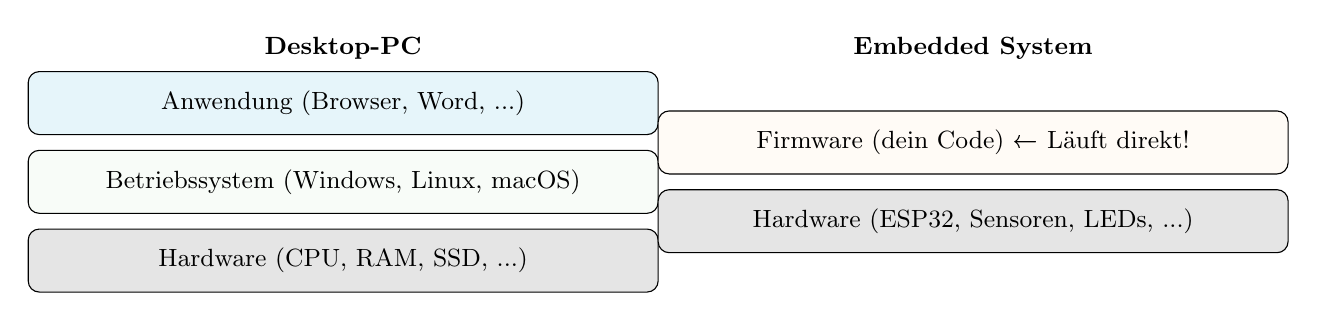
\begin{tikzpicture}[
    box/.style={draw, rounded corners, minimum width=8cm, minimum height=0.8cm, align=center, font=\small},
    label/.style={font=\small\bfseries}
  ]
    % Desktop-PC
    \node[label] at (-4,3.5) {Desktop-PC};
    \node[box, fill=InfoBoxBg] at (-4,2.8) {Anwendung (Browser, Word, ...)};
    \node[box, fill=TipBoxBg!50] at (-4,1.8) {Betriebssystem (Windows, Linux, macOS)};
    \node[box, fill=gray!20] at (-4,0.8) {Hardware (CPU, RAM, SSD, ...)};

    % Embedded System
    \node[label] at (4,3.5) {Embedded System};
    \node[box, fill=WarnBoxBg!50] at (4,2.3) {Firmware (dein Code) ← Läuft direkt!};
    \node[box, fill=gray!20] at (4,1.3) {Hardware (ESP32, Sensoren, LEDs, ...)};
  \end{tikzpicture}
  \caption{Vergleich: Desktop vs. Embedded System}
  \label{fig:cpp-desktop-vs-embedded}
\end{figure}

\textbf{Konsequenzen für den Code:}

\begin{table}[H]
  \centering
  \caption{Unterschiede zwischen Desktop- und Embedded-Entwicklung}
  \label{tab:cpp-desktop-embedded}
  \begin{tabularx}{\textwidth}{@{}l l X@{}}
    \toprule
    \textbf{Aspekt} & \textbf{Desktop} & \textbf{Embedded} \\
    \midrule
    Speicher & GBs RAM & KBs RAM \\
    Dateisystem & Ja & Meist nein \\
    Multitasking & OS regelt & Du regelst \\
    Timing & Unkritisch & Oft kritisch \\
    Fehler & Absturz → Neustart & Kann Hardware beschädigen \\
    \bottomrule
  \end{tabularx}
\end{table}

% -----------------------------------------------------------------------------
\subsection{Arduino C++: Welche Version?}
\label{subsec:cpp-version}

\subsubsection{Der Arduino-Core}

Arduino verwendet \textbf{C++11} mit Erweiterungen. Der ESP32-Arduino-Core (Espressif) basiert auf GCC 8.4 und unterstützt C++11 vollständig, C++14 und C++17 teilweise.

\subsubsection{Was Arduino hinzufügt}

Arduino ist kein eigener Compiler, sondern ein \textbf{Framework} auf C++:

\begin{lstlisting}[style=arduino,caption={Klassisches C++ vs. Arduino}]
// Klassisches C/C++: Du schreibst main()
int main() {
    // Hardware initialisieren
    while (1) {
        // Endlosschleife
    }
    return 0;
}

// Arduino: Das Framework versteckt main()
void setup() {
    // Wird einmal ausgefuehrt
}

void loop() {
    // Wird endlos wiederholt
}
\end{lstlisting}

\begin{infobox}[Hinter den Kulissen]
  Arduino's \texttt{main()} ruft \texttt{init()} für die Hardware-Initialisierung, dann \texttt{setup()}, und schließlich \texttt{loop()} in einer Endlosschleife auf.
\end{infobox}

% -----------------------------------------------------------------------------
\subsection{Programmierdogma: Embedded Best Practices}
\label{subsec:cpp-dogma}

\subsubsection{Die goldenen Regeln}

\begin{enumerate}
  \item \textbf{KEIN} dynamischer Speicher (\texttt{new}, \texttt{malloc}) in der Hauptschleife
  \item \textbf{KEINE} Blockierung (\texttt{delay} nur wenn unvermeidbar)
  \item \textbf{DETERMINISMUS:} Jeder Durchlauf dauert gleich lang
  \item \textbf{FEHLERTOLERANZ:} Hardware kann jederzeit „spinnen"
  \item \textbf{RESSOURCEN-BEWUSSTSEIN:} Jedes Byte zählt
\end{enumerate}

\subsubsection{Speicher-Dogma}

\begin{lstlisting}[style=arduino,caption={Speicherverwaltung: Schlecht vs. Gut}]
// SCHLECHT: Dynamische Allokation
void loop() {
    String text = "Hello";        // String alloziert auf Heap
    text += " World";             // Re-Allokation!
}
// -> Speicherfragmentierung, irgendwann Absturz

// GUT: Statische Allokation
static char text[32];             // Feste Groesse, einmal alloziert
void loop() {
    snprintf(text, sizeof(text), "Hello World");
}
\end{lstlisting}

\subsubsection{Timing-Dogma}

\begin{lstlisting}[style=arduino,caption={Timing: Blockierend vs. Nicht-blockierend}]
// SCHLECHT: Blockierendes Warten
void loop() {
    if (buttonPressed()) {
        doSomething();
        delay(1000);              // CPU macht 1 Sekunde NICHTS
    }
}

// GUT: Nicht-blockierendes Warten
static uint32_t lastAction = 0;
void loop() {
    if (buttonPressed() && (millis() - lastAction >= 1000)) {
        doSomething();
        lastAction = millis();
    }
}
\end{lstlisting}

\begin{warnbox}[delay() vermeiden]
  \texttt{delay()} blockiert die gesamte CPU. In dieser Zeit können keine anderen Aufgaben ausgeführt werden – keine Taster-Abfrage, keine Serial-Kommunikation, nichts.
\end{warnbox}

% -----------------------------------------------------------------------------
\subsection{Code-Aufbau: Die Anatomie der Firmware}
\label{subsec:cpp-aufbau}

\subsubsection{Dateistruktur}

\begin{lstlisting}[style=shell,numbers=none]
src/
|-- config.h      <-- Konfiguration (Konstanten, Pins)
+-- main.cpp      <-- Hauptprogramm (Logik)
\end{lstlisting}

\subsubsection{Aufbau von main.cpp}

\begin{lstlisting}[style=arduino,caption={Struktur einer Firmware-Datei}]
// 1. INCLUDES - Externe Bibliotheken einbinden
#include "config.h"
#include <SPI.h>

// 2. KONSTANTEN & KONFIGURATION
static const SPISettings spiButtons(500000, MSBFIRST, SPI_MODE1);

// 3. GLOBALE VARIABLEN (ZUSTAND)
// static = nur in dieser Datei sichtbar
static uint8_t btnRaw[BTN_BYTES];
static uint8_t activeId = 0;

// 4. HILFSFUNKTIONEN - Kleine, wiederverwendbare Bausteine
static inline bool btnIsPressed(const uint8_t *state, uint8_t id) { /* ... */ }

// 5. HARDWARE-FUNKTIONEN - Direkter Zugriff auf Peripherie
static void readButtons() { /* ... */ }

// 6. LOGIK-FUNKTIONEN - Verarbeitung, Entscheidungen
static void debounceButtons() { /* ... */ }

// 7. DEBUG-FUNKTIONEN - Ausgaben fuer Entwicklung
static void printState() { /* ... */ }

// 8. ARDUINO ENTRY POINTS
void setup() { /* Einmalige Initialisierung */ }
void loop() { /* Hauptschleife */ }
\end{lstlisting}

% -----------------------------------------------------------------------------
\subsection{C++ Syntax im Detail}
\label{subsec:cpp-syntax}

\subsubsection{Präprozessor-Direktiven}

Der Präprozessor läuft \textbf{vor} dem Compiler und manipuliert den Quelltext:

\begin{lstlisting}[style=arduino,caption={Präprozessor-Direktiven}]
// Include: Fuegt Dateiinhalt ein
#include <SPI.h>          // Sucht in System-Pfaden
#include "config.h"       // Sucht im Projekt-Ordner

// Include Guard: Verhindert doppeltes Einbinden
#pragma once              // Moderne Variante (eine Zeile)

// Alternativ (klassisch):
#ifndef CONFIG_H
#define CONFIG_H
// ... Inhalt ...
#endif
\end{lstlisting}

\subsubsection{Datentypen}

\begin{lstlisting}[style=arduino,caption={Exakte Datentypen für Embedded}]
// Embedded Best Practice: Exakte Groessen verwenden!
#include <cstdint>

int8_t   a;       //  8 Bit mit Vorzeichen:    -128 bis 127
uint8_t  b;       //  8 Bit ohne Vorzeichen:      0 bis 255
int16_t  c;       // 16 Bit mit Vorzeichen: -32768 bis 32767
uint16_t d;       // 16 Bit ohne Vorzeichen:      0 bis 65535
int32_t  e;       // 32 Bit mit Vorzeichen
uint32_t f;       // 32 Bit ohne Vorzeichen

// size_t: Fuer Groessen und Indizes (plattformabhaengig, immer positiv)
size_t arraySize = 10;
\end{lstlisting}

\begin{tipbox}[Warum exakte Größen?]
  \texttt{int} ist auf verschiedenen Plattformen unterschiedlich groß (16 oder 32 Bit). Mit \texttt{uint32\_t} ist die Größe immer 32 Bit – egal welche Plattform.
\end{tipbox}

\subsubsection{Konstanten}

\begin{lstlisting}[style=arduino,caption={Konstanten: \#define vs. constexpr}]
// C-Style (veraltet, aber funktioniert)
#define LED_COUNT 10      // Textersetzung, kein Typ!

// C++ Style (empfohlen)
const int LED_COUNT = 10;           // Zur Laufzeit, braucht RAM
constexpr int LED_COUNT = 10;       // Zur Compile-Zeit, kein RAM!

// constexpr vs const:
constexpr int COMPILE_TIME = 5 * 2;     // Berechnung zur Compile-Zeit
const int RUNTIME = analogRead(A0);      // Kann nur const sein (Laufzeit)
\end{lstlisting}

\subsubsection{Variablen-Deklaration}

\begin{lstlisting}[style=arduino,caption={Speicherklassen und static}]
// Speicherklassen
int globalVar;                    // Global: ueberall sichtbar
static int fileVar;               // Datei-lokal: nur in dieser .cpp
void func() {
    int localVar;                 // Lokal: nur in dieser Funktion
    static int persistentVar;     // Lokal, aber behaelt Wert zwischen Aufrufen!
}

// static bei lokalen Variablen:
void countCalls() {
    static int counter = 0;   // Initialisierung nur beim ersten Aufruf!
    counter++;
    Serial.println(counter);
}
// Aufruf 1: Ausgabe "1", Aufruf 2: "2", Aufruf 3: "3"
\end{lstlisting}

\subsubsection{Funktionen}

\begin{lstlisting}[style=arduino,caption={Funktionen mit Schlüsselwörtern}]
// static: Funktion nur in dieser Datei sichtbar
static void readButtons() { }

// inline: Compiler soll Code direkt einsetzen statt Funktionsaufruf
inline bool isValid(int x) { return x > 0; }

// static inline: Beides kombiniert (haeufig fuer kleine Hilfsfunktionen)
static inline uint8_t byteIndex(uint8_t id) { return (id - 1) / 8; }

// Parameter und Rueckgabe
static inline bool btnIsPressed(const uint8_t *state, uint8_t id) {
    // state: Zeiger auf Array (wird nicht veraendert wegen const)
    // id: Kopie des Wertes (call by value)
    return !(state[byte] & (1u << bit));
}
\end{lstlisting}

\subsubsection{Zeiger und Referenzen}

\begin{lstlisting}[style=arduino,caption={Zeiger, Arrays und Parameterübergabe}]
uint8_t buffer[10];           // Array
uint8_t *ptr = buffer;        // Zeiger auf erstes Element

*ptr = 42;                    // Dereferenzierung: Wert schreiben
uint8_t x = *ptr;             // Dereferenzierung: Wert lesen
ptr++;                        // Zeiger auf naechstes Element

// const-Korrektheit
const uint8_t *readOnly = buffer;    // Daten nicht aenderbar

// Funktionsparameter:
void modify(int x) { x = 99; }           // Call by Value: Kopie
void modify(int *x) { *x = 99; }         // Call by Pointer: Original
void modify(int &x) { x = 99; }          // Call by Reference: Original
void print(const String &s) { }          // Const Reference: effizient
\end{lstlisting}

\subsubsection{Bit-Operationen}

Bit-Operationen sind essentiell für Embedded-Entwicklung!

\begin{lstlisting}[style=arduino,caption={Bit-Operatoren und praktische Anwendungen}]
uint8_t a = 0b11001010;
uint8_t b = 0b10101100;

a & b     // AND:  0b10001000  (beide 1 -> 1)
a | b     // OR:   0b11101110  (mindestens einer 1 -> 1)
a ^ b     // XOR:  0b01100110  (genau einer 1 -> 1)
~a        // NOT:  0b00110101  (invertiert)
a << 2    // Links-Shift: 0b00101000 (x 4)
a >> 2    // Rechts-Shift: 0b00110010 (/ 4)

// Praktische Anwendungen:
value |= (1u << bitNr);       // Bit setzen (auf 1)
value &= ~(1u << bitNr);      // Bit loeschen (auf 0)
value ^= (1u << bitNr);       // Bit umschalten (toggle)
if (value & (1u << bitNr)) {} // Bit pruefen
\end{lstlisting}

\begin{lstlisting}[style=arduino,caption={Bit-Operationen im Selection Panel}]
// Taster gedrueckt pruefen (Active-Low: 0 = gedrueckt)
return !(state[byte] & (1u << bit));
//       ^              ^
//       Invertieren    Bit-Maske

// LED einschalten
ledState[byte] |= (1u << bit);

// LED ausschalten
ledState[byte] &= ~(1u << bit);
\end{lstlisting}

\subsubsection{Kontrollstrukturen}

\begin{lstlisting}[style=arduino,caption={Schleifen und Kontrollfluss}]
// for-Schleife
for (int i = 0; i < 10; i++) {
    // i laeuft von 0 bis 9
}

// Rueckwaerts (wichtig fuer Daisy-Chain!)
for (int i = LED_BYTES - 1; i >= 0; --i) {
    SPI.transfer(ledState[i]);
}

// Fruehes Verlassen
for (int i = 0; i < 100; i++) {
    if (found) break;         // Schleife sofort verlassen
    if (skip) continue;       // Zum naechsten Durchlauf springen
}

// Ternaerer Operator
int max = (a > b) ? a : b;
\end{lstlisting}

\subsubsection{Speicher-Funktionen}

\begin{lstlisting}[style=arduino,caption={memcpy, memset, memcmp}]
#include <cstring>

uint8_t src[10] = {1, 2, 3};
uint8_t dst[10];

memcpy(dst, src, 10);         // 10 Bytes von src nach dst kopieren
memset(dst, 0x00, 10);        // 10 Bytes mit 0x00 fuellen
memset(dst, 0xFF, 10);        // 10 Bytes mit 0xFF fuellen

if (memcmp(src, dst, 10) == 0) {
    // Identisch
}
\end{lstlisting}

% -----------------------------------------------------------------------------
\subsection{Arduino-spezifische Funktionen}
\label{subsec:cpp-arduino-funktionen}

\begin{table}[H]
  \centering
  \caption{Wichtige Arduino-Funktionen}
  \label{tab:cpp-arduino-funktionen}
  \begin{tabularx}{\textwidth}{@{}l X@{}}
    \toprule
    \textbf{Funktion} & \textbf{Beschreibung} \\
    \midrule
    \multicolumn{2}{@{}l}{\textit{Digitale I/O}} \\
    \texttt{pinMode(PIN, MODE)} & MODE: INPUT, OUTPUT, INPUT\_PULLUP \\
    \texttt{digitalWrite(PIN, val)} & HIGH oder LOW setzen \\
    \texttt{digitalRead(PIN)} & HIGH oder LOW lesen \\
    \midrule
    \multicolumn{2}{@{}l}{\textit{Timing}} \\
    \texttt{delay(ms)} & Warten (BLOCKIEREND!) \\
    \texttt{delayMicroseconds(us)} & Warten in µs (BLOCKIEREND!) \\
    \texttt{millis()} & Millisekunden seit Start \\
    \texttt{micros()} & Mikrosekunden seit Start \\
    \midrule
    \multicolumn{2}{@{}l}{\textit{Serial}} \\
    \texttt{Serial.begin(baud)} & Baudrate setzen \\
    \texttt{Serial.print(x)} & Ohne Zeilenumbruch \\
    \texttt{Serial.println(x)} & Mit Zeilenumbruch \\
    \texttt{Serial.printf(...)} & Formatiert (ESP32) \\
    \midrule
    \multicolumn{2}{@{}l}{\textit{SPI}} \\
    \texttt{SPI.begin(SCK, MISO, MOSI, SS)} & Pins konfigurieren \\
    \texttt{SPI.beginTransaction(settings)} & Transaktion starten \\
    \texttt{SPI.transfer(byte)} & Byte senden/empfangen \\
    \texttt{SPI.endTransaction()} & Transaktion beenden \\
    \midrule
    \multicolumn{2}{@{}l}{\textit{PWM (ESP32)}} \\
    \texttt{ledcSetup(ch, freq, res)} & Kanal konfigurieren \\
    \texttt{ledcAttachPin(pin, ch)} & Pin zuweisen \\
    \texttt{ledcWrite(ch, duty)} & Duty Cycle setzen \\
    \bottomrule
  \end{tabularx}
\end{table}

% -----------------------------------------------------------------------------
\subsection{Der Code im Kontext}
\label{subsec:cpp-kontext}

\subsubsection{Ablaufdiagramm}

\begin{figure}[H]
  \centering
  \begin{tikzpicture}[
    box/.style={draw, rounded corners, minimum width=3cm, minimum height=0.8cm, align=center, font=\small},
    arrow/.style={->, >=Stealth, thick}
  ]
    % Setup
    \node[box, fill=InfoBoxBg, minimum width=8cm] (setup) at (0,5) {\textbf{setup()}};
    \node[font=\tiny, align=left, right=0.5cm of setup] {
      Serial.begin()\\
      pinMode()\\
      SPI.begin()\\
      ledcSetup()
    };

    % Loop boxes
    \node[box, fill=TipBoxBg!50] (read) at (0,3.5) {readButtons()};
    \node[box, fill=TipBoxBg!50] (debounce) at (0,2.5) {debounceButtons()};
    \node[box, fill=TipBoxBg!50] (update) at (0,1.5) {updateActiveId()};
    \node[box, fill=TipBoxBg!50] (led) at (0,0.5) {writeLEDs()};
    \node[box, fill=gray!20] (delay) at (0,-0.5) {delay(2)};

    % Arrows
    \draw[arrow] (setup) -- (read);
    \draw[arrow] (read) -- (debounce);
    \draw[arrow] (debounce) -- (update);
    \draw[arrow] (update) -- (led);
    \draw[arrow] (led) -- (delay);
    \draw[arrow] (delay.west) -- ++(-1.5,0) |- (read.west);

    % Labels
    \node[font=\tiny, right=0.3cm of read] {Hardware → btnRaw[]};
    \node[font=\tiny, right=0.3cm of debounce] {btnRaw[] → btnDebounced[]};
    \node[font=\tiny, right=0.3cm of update] {btnDebounced[] → activeId};
    \node[font=\tiny, right=0.3cm of led] {activeId → Hardware};
  \end{tikzpicture}
  \caption{Ablauf der Firmware-Hauptschleife}
  \label{fig:cpp-ablauf}
\end{figure}

\subsubsection{Datenfluss}

\begin{lstlisting}[style=shell,numbers=none]
Hardware          Firmware                    Hardware
---------         --------                    --------
Taster ----------> btnRaw[]
                      |
                      v
                  btnDebounced[] (zeitverzoegert, stabil)
                      |
                      v
                  activeId (0-10)
                      |
                      v
                  ledState[]
                      |
                      v
                                --------------> LEDs
\end{lstlisting}

% -----------------------------------------------------------------------------
\subsection{Zusammenfassung}
\label{subsec:cpp-zusammenfassung}

\subsubsection{Checkliste für guten Embedded-Code}

\begin{itemize}
  \item[$\square$] Exakte Datentypen verwenden (\texttt{uint8\_t}, \texttt{uint32\_t}, ...)
  \item[$\square$] \texttt{static} für datei-lokale Variablen und Funktionen
  \item[$\square$] \texttt{constexpr} für Compile-Zeit-Konstanten
  \item[$\square$] Kein dynamischer Speicher in \texttt{loop()}
  \item[$\square$] Blockierende Wartezeiten vermeiden
  \item[$\square$] Bit-Operationen statt Division/Multiplikation wo möglich
  \item[$\square$] Fehlerprüfung bei Parametern (Range-Checks)
  \item[$\square$] Aussagekräftige Namen (nicht \texttt{x}, \texttt{temp}, \texttt{data})
  \item[$\square$] Kommentare erklären WARUM, nicht WAS
\end{itemize}

\subsubsection{Schnellreferenz: Schlüsselwörter}

\begin{table}[H]
  \centering
  \caption{C++ Schlüsselwörter für Embedded}
  \label{tab:cpp-schluesselwoerter}
  \begin{tabularx}{\textwidth}{@{}l X@{}}
    \toprule
    \textbf{Schlüsselwort} & \textbf{Bedeutung} \\
    \midrule
    \texttt{static} & Datei-lokal (global) oder persistent (lokal) \\
    \texttt{const} & Wert nicht änderbar (zur Laufzeit) \\
    \texttt{constexpr} & Wert zur Compile-Zeit berechnet \\
    \texttt{inline} & Compiler-Hinweis: Code direkt einsetzen \\
    \texttt{volatile} & Wert kann sich „von außen" ändern (Hardware, ISR) \\
    \texttt{void} & Kein Rückgabewert / generischer Zeiger \\
    \bottomrule
  \end{tabularx}
\end{table}

% =============================================================================
% FIRMWARE-CODE-GUIDE.tex – Firmware-Architektur und Modul-Referenz
% Modulares Fragment (kein \documentclass, kein \begin{document})
% Stand: 2026-01-08 | Version: 2.5.2
% =============================================================================

\section{Firmware Code Guide}
\label{sec:firmware-code-guide}

Wie ist die Firmware des Selection Panels aufgebaut? Dieser Guide dokumentiert die Architektur, die Module und die Designentscheidungen der ESP32-S3-Firmware.

% -----------------------------------------------------------------------------
\subsection{Projektstruktur}
\label{subsec:fw-projektstruktur}

\begin{lstlisting}[style=shell,numbers=none]
firmware/
|-- include/
|   |-- bitops.h        # Bit-Adressierung fuer Taster/LEDs
|   |-- config.h        # Zentrale Konfiguration
|   +-- types.h         # Gemeinsame Datentypen
|-- src/
|   |-- main.cpp        # Entry Point
|   |-- app/
|   |   |-- io_task.cpp/.h      # I/O-Verarbeitung
|   |   +-- serial_task.cpp/.h  # Protokoll-Handler
|   |-- drivers/
|   |   |-- cd4021.cpp/.h       # Taster-Schieberegister
|   |   +-- hc595.cpp/.h        # LED-Schieberegister
|   |-- hal/
|   |   +-- spi_bus.cpp/.h      # SPI-Abstraktion
|   +-- logic/
|       |-- debounce.cpp/.h     # Entprellung
|       +-- selection.cpp/.h    # Auswahl-Logik
+-- platformio.ini
\end{lstlisting}

% -----------------------------------------------------------------------------
\subsection{Schichtenmodell}
\label{subsec:fw-schichtenmodell}

Die Firmware folgt einem strikten Schichtenmodell. Abhängigkeiten zeigen nur nach unten – eine Schicht kennt nur die darunterliegende.

\begin{figure}[H]
  \centering
  \begin{tikzpicture}[
    layer/.style={draw, rounded corners, minimum width=10cm, minimum height=1.2cm, align=center, font=\small},
    arrow/.style={->, >=Stealth, thick}
  ]
    % Layers
    \node[layer, fill=InfoBoxBg] (main) at (0,6) {\textbf{main.cpp}\\Queue erstellen, Tasks starten};
    \node[layer, fill=TipBoxBg!50] (app) at (0,4.5) {\textbf{app/}\\io\_task.cpp \quad serial\_task.cpp};
    \node[layer, fill=CodeBackground] (logic) at (0,3) {\textbf{logic/}\\debounce.cpp \quad selection.cpp};
    \node[layer, fill=WarnBoxBg!30] (drivers) at (0,1.5) {\textbf{drivers/}\\cd4021.cpp \quad hc595.cpp};
    \node[layer, fill=gray!20] (hal) at (0,0) {\textbf{hal/}\\spi\_bus.cpp (Mutex-geschützt)};

    % Arrows
    \draw[arrow] (main) -- (app);
    \draw[arrow] (app) -- (logic);
    \draw[arrow] (logic) -- (drivers);
    \draw[arrow] (drivers) -- (hal);
  \end{tikzpicture}
  \caption{Schichtenmodell der Firmware}
  \label{fig:fw-schichtenmodell}
\end{figure}

% -----------------------------------------------------------------------------
\subsection{Modul-Referenz}
\label{subsec:fw-module}

\subsubsection{config.h – Zentrale Konfiguration}

Alle Hardware- und Timing-Parameter an einer Stelle:

\begin{lstlisting}[style=arduino,caption={Zentrale Konfiguration in config.h}]
// Anzahl der Ein-/Ausgaenge
constexpr uint8_t BTN_COUNT = 10;
constexpr uint8_t LED_COUNT = 10;

// Bytes fuer Bit-Arrays (aufrunden: 10 Bits -> 2 Bytes)
constexpr size_t BTN_BYTES = (BTN_COUNT + 7) / 8;
constexpr size_t LED_BYTES = (LED_COUNT + 7) / 8;

// Pin-Zuordnung (gemeinsamer SPI-Bus)
constexpr int PIN_SCK      = D8;   // SPI-Takt (shared)
constexpr int PIN_BTN_PS   = D1;   // CD4021B: Parallel/Serial Select
constexpr int PIN_BTN_MISO = D9;   // CD4021B: Daten (Q8)
constexpr int PIN_LED_MOSI = D10;  // 74HC595: Daten (SER)
constexpr int PIN_LED_RCK  = D0;   // 74HC595: Latch (RCLK)
constexpr int PIN_LED_OE   = D2;   // 74HC595: Output Enable (PWM)

// Timing
constexpr uint32_t IO_PERIOD_MS = 5;   // 200 Hz Abtastrate
constexpr uint32_t DEBOUNCE_MS = 30;   // Entprellzeit

// SPI-Einstellungen
constexpr uint32_t SPI_HZ_BTN = 500000UL;  // 500 kHz (CD4021B)
constexpr uint32_t SPI_HZ_LED = 1000000UL; // 1 MHz (74HC595)
constexpr uint8_t SPI_MODE_BTN = SPI_MODE1; // CPOL=0, CPHA=1
constexpr uint8_t SPI_MODE_LED = SPI_MODE0; // CPOL=0, CPHA=0
\end{lstlisting}

\subsubsection{bitops.h – Bit-Adressierung}

Dieses Modul abstrahiert die Hardware-Verdrahtung der Schieberegister.

\begin{lstlisting}[style=arduino,caption={Bit-Adressierung für Taster und LEDs}]
// CD4021B Button Bit-Mapping
// Hardware-Verdrahtung: BTN 1 -> PI-8 (Pin 1), BTN 8 -> PI-1 (Pin 7)
// Formel: btn_bit(id) = (id - 1) % 8
static inline uint8_t btn_byte(uint8_t id) { return (id - 1) / 8; }
static inline uint8_t btn_bit(uint8_t id)  { return (id - 1) % 8; }

// 74HC595 LED Bit-Mapping
// Hardware-Verdrahtung: LED 1 -> QA (Bit 0), LED 8 -> QH (Bit 7)
static inline uint8_t led_byte(uint8_t id) { return (id - 1) / 8; }
static inline uint8_t led_bit(uint8_t id)  { return (id - 1) % 8; }

// Active-Low Hilfsfunktionen (Taster: 0 = gedrueckt, Pull-up!)
static inline bool activeLow_pressed(const uint8_t* arr, uint8_t id) {
    return !((arr[btn_byte(id)] >> btn_bit(id)) & 1);
}

// LED-Hilfsfunktionen
static inline void led_set(uint8_t* arr, uint8_t id, bool on) {
    uint8_t mask = 1 << led_bit(id);
    if (on) arr[led_byte(id)] |= mask;
    else    arr[led_byte(id)] &= ~mask;
}
\end{lstlisting}

\subsubsection{types.h – Gemeinsame Datentypen}

\begin{lstlisting}[style=arduino,caption={LogEvent-Struktur für die Queue}]
struct LogEvent {
    uint32_t ms;                // Zeitstempel
    uint8_t raw[BTN_BYTES];     // Rohzustand der Taster
    uint8_t deb[BTN_BYTES];     // Entprellter Zustand
    uint8_t led[LED_BYTES];     // LED-Ausgabezustand
    uint8_t activeId;           // Aktive Auswahl (0 = keine, 1-10 = ID)
    bool rawChanged;            // Flag: Raw hat sich geaendert
    bool debChanged;            // Flag: Debounced hat sich geaendert
    bool activeChanged;         // Flag: Auswahl hat sich geaendert
};
\end{lstlisting}

\subsubsection{spi\_bus.h – HAL-Schicht}

\begin{lstlisting}[style=arduino,caption={Mutex-geschützte SPI-Abstraktion}]
class SpiBus {
public:
    void begin(int sck, int miso, int mosi);
    void lock();    // Mutex nehmen
    void unlock();  // Mutex freigeben
private:
    SemaphoreHandle_t mtx_;
};

// RAII Guard fuer automatisches Cleanup
class SpiGuard {
public:
    SpiGuard(SpiBus& bus, const SPISettings& settings);
    ~SpiGuard();  // Automatisch: endTransaction() + unlock()
};
\end{lstlisting}

\subsubsection{cd4021.h – Taster-Treiber}

\begin{lstlisting}[style=arduino,caption={CD4021B-Treiber mit First-Bit-Rescue}]
void Cd4021::readRaw(SpiBus& bus, uint8_t* out) {
    // 1. Parallel Load
    digitalWrite(PIN_BTN_PS, HIGH);
    delayMicroseconds(2);
    digitalWrite(PIN_BTN_PS, LOW);
    delayMicroseconds(2);

    // 2. First Bit Rescue: PI-1 liegt bereits an Q8!
    uint8_t firstBit = digitalRead(PIN_BTN_MISO);

    // 3. SPI Transfer (restliche Bits)
    SpiGuard g(bus, spi_);
    SPI.transfer(out, BTN_BYTES);

    // 4. First Bit einsetzen (MSB von Byte 0)
    out[0] = (out[0] >> 1) | (firstBit << 7);
}
\end{lstlisting}

\begin{infobox}[First-Bit-Problem]
  Nach dem Parallel-Load (P/S HIGH→LOW) liegt das erste Bit (PI-1) bereits an Q8 an – bevor der erste Clock kommt. Die Lösung: \texttt{digitalRead()} vor dem SPI-Transfer.
\end{infobox}

\subsubsection{debounce.h – Entprellung}

Der Algorithmus ist zeitbasiert:

\begin{enumerate}
  \item Bei Rohwert-Änderung: Timer zurücksetzen
  \item Wenn Timer $\geq$ \SI{30}{\milli\second} UND Rohwert $\neq$ entprellt: übernehmen
\end{enumerate}

\begin{lstlisting}[style=arduino,caption={Debouncer-Klasse}]
class Debouncer {
public:
    void init();
    bool update(uint32_t nowMs, const uint8_t* raw, uint8_t* deb);
private:
    uint8_t rawPrev_[BTN_BYTES];
    uint32_t lastChange_[BTN_COUNT];  // Timer pro Taster
};
\end{lstlisting}

\subsubsection{selection.h – Auswahl-Logik}

Prinzip: „Last Press Wins" – der zuletzt gedrückte Taster wird aktiv.

\begin{lstlisting}[style=arduino,caption={Selection-Klasse}]
class Selection {
public:
    void init();
    bool update(const uint8_t* debNow, uint8_t& activeId);
private:
    uint8_t debPrev_[BTN_BYTES];
};
\end{lstlisting}

\begin{tipbox}[Latch-Modus]
  Mit \texttt{LATCH\_SELECTION = true} bleibt die Auswahl nach Loslassen bestehen.
\end{tipbox}

% -----------------------------------------------------------------------------
\subsection{FreeRTOS-Konfiguration}
\label{subsec:fw-freertos}

\begin{table}[H]
  \centering
  \caption{FreeRTOS Tasks}
  \label{tab:fw-tasks}
  \begin{tabularx}{\textwidth}{@{}l r r r X@{}}
    \toprule
    \textbf{Task} & \textbf{Core} & \textbf{Priorität} & \textbf{Periode} & \textbf{Funktion} \\
    \midrule
    io\_task & 1 & 5 & \SI{5}{\milli\second} & Hardware-I/O (Taster, LEDs) \\
    serial\_task & 1 & 2 & Event-driven & Protokoll-Handler \\
    \bottomrule
  \end{tabularx}
\end{table}

Core 0 bleibt für WiFi/BLE reserviert (falls später benötigt).

% -----------------------------------------------------------------------------
\subsection{Datenfluss im Detail}
\label{subsec:fw-datenfluss}

Was passiert in jedem I/O-Zyklus? Schauen wir uns die Hauptschleife an:

\begin{lstlisting}[style=arduino,caption={I/O-Task Hauptschleife (vereinfacht)}]
void io_loop() {
    TickType_t lastWake = xTaskGetTickCount();

    while (true) {
        uint32_t now = millis();

        // 1. Taster einlesen
        cd4021.readRaw(bus, raw);
        bool rawChg = memcmp(raw, rawPrev, BTN_BYTES) != 0;

        // 2. Entprellen
        bool debChg = debouncer.update(now, raw, deb);

        // 3. Auswahl aktualisieren
        bool selChg = selection.update(deb, activeId);

        // 4. LEDs setzen (activeId -> One-Hot)
        memset(led, 0, LED_BYTES);
        if (activeId > 0) led_set(led, activeId, true);
        hc595.write(bus, led);

        // 5. Bei Aenderung: Event senden
        if (debChg || selChg) {
            LogEvent ev = {now, raw, deb, led, activeId, ...};
            xQueueSend(queue, &ev, 0);
        }

        // 6. Auf naechsten Zyklus warten
        vTaskDelayUntil(&lastWake, pdMS_TO_TICKS(IO_PERIOD_MS));
    }
}
\end{lstlisting}

% -----------------------------------------------------------------------------
\subsection{Design-Entscheidungen}
\label{subsec:fw-design}

\subsubsection{Warum Queue statt direktem Serial-Aufruf?}

Die Queue entkoppelt I/O von Serial-Ausgabe:

\begin{itemize}
  \item io\_task blockiert nie (\SI{5}{\milli\second} Deadline)
  \item serial\_task kann langsam sein (USB-Puffer voll)
  \item Atomare Snapshots (keine Race-Conditions)
\end{itemize}

\subsubsection{Warum SpiGuard (RAII)?}

Garantiert korrektes Cleanup auch bei frühem Return:

\begin{lstlisting}[style=arduino,caption={RAII-Pattern für SPI}]
{
    SpiGuard g(bus, settings);
    if (error) return;  // endTransaction() + unlock() trotzdem!
    SPI.transfer(data);
}
\end{lstlisting}

\subsubsection{Warum zeitbasiertes Debouncing?}

\begin{itemize}
  \item Unabhängig von Abtastrate
  \item Jeder Taster hat eigenen Timer
  \item Schnelle Tastenfolgen möglich
\end{itemize}

\subsubsection{Warum LED\_REFRESH\_EVERY\_CYCLE?}

Beim CD4021B-Read werden Nullen durch den 74HC595 getaktet (gemeinsamer SCK). Ein glitchender Latch-Pin könnte LEDs kurz ausschalten. Der Refresh nach jedem Zyklus kompensiert dies.

% -----------------------------------------------------------------------------
\subsection{Skalierung auf 100 Buttons}
\label{subsec:fw-skalierung}

Die Architektur skaliert durch Änderung zweier Konstanten:

\begin{lstlisting}[style=arduino,caption={Skalierung auf 100 Buttons}]
constexpr uint8_t BTN_COUNT = 100;
constexpr uint8_t LED_COUNT = 100;
// BTN_BYTES und LED_BYTES werden automatisch auf 13 berechnet
\end{lstlisting}

Alle Schleifen und Bit-Arrays passen sich automatisch an. Die SPI-Transferzeit steigt von $\sim$\SI{40}{\micro\second} auf $\sim$\SI{320}{\micro\second} – weit unter dem \SI{5}{\milli\second}-Budget.

% -----------------------------------------------------------------------------
\subsection{Build und Upload}
\label{subsec:fw-build}

\begin{lstlisting}[style=shell]
# PlatformIO
cd firmware
pio run -t upload
pio device monitor

# Serial-Ausgabe
# READY
# FW SelectionPanel v2.5.2
# PRESS 001
# RELEASE 001
\end{lstlisting}

% -----------------------------------------------------------------------------
\subsection{Debugging}
\label{subsec:fw-debugging}

\subsubsection{Log-Level aktivieren}

In \filep{config.h}:

\begin{lstlisting}[style=arduino,caption={Debug-Optionen}]
constexpr bool LOG_VERBOSE_PER_ID = true;   // Details pro Taster
constexpr bool LOG_ON_RAW_CHANGE = true;    // Rohwert-Aenderungen
constexpr bool SERIAL_PROTOCOL_ONLY = false; // Debug-Ausgabe erlauben
\end{lstlisting}

\subsubsection{Bit-Mapping verifizieren}

\begin{lstlisting}[style=shell]
# STATUS-Befehl zeigt Bit-Arrays:
echo "STATUS" > /dev/serial/by-id/usb-Espressif*

# Ausgabe:
# LEDS 0000000001    <-- LED 1 an (Bit 0)
# BTNS 1111111110    <-- BTN 1 gedrueckt (Active-Low: Bit 0 = 0)
\end{lstlisting}

\begin{table}[H]
  \centering
  \caption{Serial-Protokoll für Debugging}
  \label{tab:fw-debug-protokoll}
  \begin{tabularx}{\textwidth}{@{}l l X@{}}
    \toprule
    \textbf{Befehl} & \textbf{Antwort} & \textbf{Beschreibung} \\
    \midrule
    \texttt{STATUS} & \texttt{LEDS .../BTNS ...} & Bit-Arrays anzeigen \\
    \texttt{PING} & \texttt{PONG} & Verbindungstest \\
    \texttt{LEDSET 005} & \texttt{OK} & LED 5 setzen (One-Hot) \\
    \texttt{LEDCLR} & \texttt{OK} & Alle LEDs aus \\
    \bottomrule
  \end{tabularx}
\end{table}


% --- Server & Dashboard (Raspberry Pi) ---
% =============================================================================
% PI-INTEGRATION.tex – Raspberry Pi 5 Integration (Phase 7)
% Modulares Fragment (kein \documentclass, kein \begin{document})
% Stand: 2026-01-08 | Version: 2.5.2
% =============================================================================

\section{Raspberry Pi Integration}
\label{sec:pi-integration}

In Phase 7 wird der ESP32-S3 zum reinen I/O-Controller. Der Raspberry Pi 5 übernimmt die Anwendungslogik: Er empfängt Taster-Events über Serial, sendet sie per WebSocket an das Web-Dashboard und steuert bei Bedarf die LEDs. Wie funktioniert diese Arbeitsteilung?

% -----------------------------------------------------------------------------
\subsection{Systemübersicht}
\label{subsec:pi-systemuebersicht}

\begin{figure}[H]
  \centering
  \begin{tikzpicture}[
    box/.style={draw, rounded corners, minimum width=3cm, minimum height=1.2cm, align=center, font=\small},
    bigbox/.style={draw, rounded corners, minimum width=11cm, minimum height=2cm, align=center},
    arrow/.style={->, >=Stealth, thick},
    label/.style={font=\tiny, align=center}
  ]
    % Raspberry Pi Box
    \node[bigbox, fill=InfoBoxBg] (pi) at (0,3) {
      \textbf{Raspberry Pi 5}\\
      \small server.py (aiohttp) – Serial-Thread ↔ Asyncio Event Loop
    };

    % Endpoints
    \node[box, fill=CodeBackground] (static) at (-4,0.5) {\texttt{/static/}\\app.js, CSS};
    \node[box, fill=CodeBackground] (ws) at (0,0.5) {\texttt{/ws}\\WebSocket};
    \node[box, fill=CodeBackground] (media) at (4,0.5) {\texttt{/media/}\\001.jpg/.mp3};

    % ESP32
    \node[bigbox, fill=TipBoxBg, minimum height=1.5cm] (esp) at (0,-2) {
      \textbf{ESP32-S3 (XIAO)}\\
      \small PRESS/RELEASE Events → Serial TX | LED-Steuerung ← Serial RX
    };

    % Verbindungen
    \draw[arrow] (pi) -- (static);
    \draw[arrow] (pi) -- (ws);
    \draw[arrow] (pi) -- (media);
    \draw[arrow, <->] (pi) -- node[right, font=\tiny] {USB-CDC @ \SI{115200}{\baud}} (esp);
  \end{tikzpicture}
  \caption{Systemarchitektur der Pi-Integration}
  \label{fig:pi-systemarchitektur}
\end{figure}

\begin{infobox}[Lokale LED-Steuerung]
  Mit \texttt{ESP32\_SETS\_LED\_LOCALLY = true} setzt der ESP32 die LED bei Tastendruck selbst. Der Server muss dann nur noch \texttt{LEDCLR} nach Audio-Ende senden. Das reduziert die Latenz auf unter \SI{5}{\milli\second}.
\end{infobox}

% -----------------------------------------------------------------------------
\subsection{Serial-Verbindung}
\label{subsec:pi-serial}

\subsubsection{Stabiler Device-Pfad (by-id)}

Der ESP32-S3 erscheint als USB-CDC-Gerät. Der Pfad \filep{/dev/ttyACM0} kann sich nach einem Reboot ändern – ein klassisches Problem. Die Lösung: Wir verwenden den stabilen by-id-Pfad.

\begin{lstlisting}[style=shell]
# Stabilen Pfad ermitteln
ls -la /dev/serial/by-id/
# Ausgabe: usb-Espressif_USB_JTAG_serial_debug_unit_98:3D:AE:EA:08:1C-if00

# Dieser Pfad bleibt stabil
SERIAL_PORT="/dev/serial/by-id/usb-Espressif_USB_JTAG_serial_debug_unit_98:3D:AE:EA:08:1C-if00"
\end{lstlisting}

\subsubsection{Berechtigungen}

\begin{lstlisting}[style=shell]
# Benutzer zur dialout-Gruppe hinzufuegen
sudo usermod -aG dialout $USER
# Ausloggen und wieder einloggen!

# Verbindung testen
screen $SERIAL_PORT 115200
# Erwartete Ausgabe:
# READY
# FW SelectionPanel v2.5.2
\end{lstlisting}

\begin{warnbox}[Neu einloggen erforderlich]
  Gruppenmitgliedschaften werden erst nach einem neuen Login aktiv. Ein einfaches \texttt{exit} und erneutes \texttt{ssh rover} genügt.
\end{warnbox}

% -----------------------------------------------------------------------------
\subsection{Server-Architektur}
\label{subsec:pi-server-architektur}

Der Python-Server verwendet \textbf{aiohttp} für asynchrone HTTP/WebSocket-Verarbeitung. \Cref{tab:pi-komponenten} zeigt die Komponenten.

\begin{table}[H]
  \centering
  \caption{Server-Komponenten und ihre Technologien}
  \label{tab:pi-komponenten}
  \begin{tabularx}{\textwidth}{@{}l l X@{}}
    \toprule
    \textbf{Komponente} & \textbf{Technologie} & \textbf{Funktion} \\
    \midrule
    HTTP-Server & aiohttp & Statische Dateien, API-Endpoints \\
    WebSocket & aiohttp & Echtzeit-Kommunikation mit Browser \\
    Serial-Reader & Threading & Liest ESP32-Events im Hintergrund \\
    Media-Validator & Startup & Prüft ob alle Medien vorhanden \\
    \bottomrule
  \end{tabularx}
\end{table}

\subsubsection{HTTP-Endpoints}

\begin{table}[H]
  \centering
  \caption{HTTP-Endpoints des Servers}
  \label{tab:pi-endpoints}
  \begin{tabularx}{\textwidth}{@{}l l X@{}}
    \toprule
    \textbf{Endpoint} & \textbf{Methode} & \textbf{Beschreibung} \\
    \midrule
    \texttt{/} & GET & Web-Dashboard (index.html) \\
    \texttt{/ws} & WebSocket & Echtzeit-Events \\
    \texttt{/static/} & GET & JavaScript, CSS, Favicon \\
    \texttt{/media/} & GET & Bilder und Audio (001.jpg, 001.mp3) \\
    \texttt{/status} & GET & Server-Status als JSON \\
    \texttt{/health} & GET & Health-Check (für Monitoring) \\
    \texttt{/test/play/\{id\}} & GET & Simuliert Tastendruck \\
    \texttt{/test/stop} & GET & Stoppt Wiedergabe \\
    \bottomrule
  \end{tabularx}
\end{table}

\subsubsection{Konfiguration}

\begin{lstlisting}[style=python,caption={Wichtige Einstellungen in server.py}]
VERSION = "2.5.2"

# Build-Modus
PROTOTYPE_MODE = True   # True = 10 Medien, False = 100 Medien
NUM_MEDIA = 10 if PROTOTYPE_MODE else 100

# Serial-Port (stabiler by-id Pfad!)
SERIAL_PORT = "/dev/serial/by-id/usb-Espressif_USB_JTAG_..."
SERIAL_BAUD = 115200

# HTTP-Server
HTTP_HOST = "0.0.0.0"
HTTP_PORT = 8080

# ESP32 setzt LED selbst bei Tastendruck
ESP32_SETS_LED_LOCALLY = True
\end{lstlisting}

% -----------------------------------------------------------------------------
\subsection{Protokolle}
\label{subsec:pi-protokolle}

\subsubsection{WebSocket-Protokoll (Server ↔ Browser)}

\begin{table}[H]
  \centering
  \caption{WebSocket-Nachrichten}
  \label{tab:pi-websocket}
  \begin{tabularx}{\textwidth}{@{}l l l X@{}}
    \toprule
    \textbf{Richtung} & \textbf{Type} & \textbf{Beispiel} & \textbf{Beschreibung} \\
    \midrule
    Server → Browser & play & \texttt{\{"type":"play","id":3\}} & Wiedergabe starten \\
    Server → Browser & stop & \texttt{\{"type":"stop"\}} & Wiedergabe stoppen \\
    Browser → Server & ended & \texttt{\{"type":"ended","id":3\}} & Audio beendet \\
    Browser → Server & ping & \texttt{\{"type":"ping"\}} & Heartbeat \\
    \bottomrule
  \end{tabularx}
\end{table}

\subsubsection{Serial-Protokoll (ESP32 ↔ Pi)}

\begin{table}[H]
  \centering
  \caption{Serial-Nachrichten zwischen ESP32 und Pi}
  \label{tab:pi-serial-protokoll}
  \begin{tabularx}{\textwidth}{@{}l l l X@{}}
    \toprule
    \textbf{Richtung} & \textbf{Nachricht} & \textbf{Beispiel} & \textbf{Bedeutung} \\
    \midrule
    ESP32 → Pi & READY & \texttt{READY} & ESP32 bereit \\
    ESP32 → Pi & FW & \texttt{FW SelectionPanel v2.5.2} & Firmware-Version \\
    ESP32 → Pi & PRESS & \texttt{PRESS 001} & Taster gedrückt \\
    ESP32 → Pi & RELEASE & \texttt{RELEASE 001} & Taster losgelassen \\
    Pi → ESP32 & LEDSET & \texttt{LEDSET 001} & One-Hot LED (optional) \\
    Pi → ESP32 & LEDCLR & \texttt{LEDCLR} & Alle LEDs aus \\
    \bottomrule
  \end{tabularx}
\end{table}

\begin{tipbox}[LED-Steuerung]
  Mit \texttt{ESP32\_SETS\_LED\_LOCALLY = true} setzt der ESP32 die LED bei Tastendruck selbst. Der Server sendet dann nur \texttt{LEDCLR} nach Audio-Ende.
\end{tipbox}

% -----------------------------------------------------------------------------
\subsection{Datenfluss}
\label{subsec:pi-datenfluss}

Was passiert, wenn wir Taster 3 drücken? Der Datenfluss durchläuft mehrere Stationen:

\begin{enumerate}
  \item \textbf{ESP32:} Entprellt den Taster, schaltet LED 3 an, sendet \texttt{PRESS 003}
  \item \textbf{Serial-Thread:} Empfängt die Nachricht, gibt sie an den Event Loop
  \item \textbf{Event Loop:} Broadcastet \texttt{\{"type":"play","id":3\}} an alle WebSocket-Clients
  \item \textbf{Browser:} Zeigt Bild 003.jpg, spielt 003.mp3 ab
  \item \textbf{Browser:} Sendet nach Audio-Ende \texttt{\{"type":"ended","id":3\}}
  \item \textbf{Server:} Sendet \texttt{LEDCLR} an ESP32 (falls ID noch aktuell)
  \item \textbf{ESP32:} Schaltet alle LEDs aus
\end{enumerate}

% -----------------------------------------------------------------------------
\subsection{Web-Dashboard}
\label{subsec:pi-dashboard}

Das Dashboard (\filep{index.html} + \filep{app.js}) bietet folgende Features:

\begin{itemize}
  \item \textbf{Audio-Unlock:} Button zum Entsperren der Browser-Autoplay-Policy
  \item \textbf{Medien-Preload:} Lädt alle Bilder/Audio nach Unlock vor
  \item \textbf{Echtzeit-Anzeige:} Aktuelles Bild + Audio-Fortschritt
  \item \textbf{Keyboard-Shortcuts:} Space = Play/Pause, Ctrl+D = Debug
  \item \textbf{Debug-Panel:} Zeigt alle Events (ausklappbar)
\end{itemize}

\subsubsection{Zugriff}

\begin{lstlisting}[style=shell]
# Server starten
cd /home/pi/selection-panel
python3 server.py

# Browser oeffnen
# Lokal:   http://localhost:8080/
# LAN:     http://rover:8080/
# IP:      http://192.168.1.24:8080/
\end{lstlisting}

\subsubsection{Status-API}

\begin{lstlisting}[style=shell]
curl http://rover:8080/status | jq
\end{lstlisting}

\begin{lstlisting}[style=json,caption={Beispiel-Antwort von /status}]
{
  "version": "2.5.2",
  "mode": "prototype",
  "num_media": 10,
  "current_button": null,
  "ws_clients": 1,
  "serial_connected": true,
  "serial_port": "/dev/serial/by-id/...",
  "media_missing": 0,
  "esp32_local_led": true
}
\end{lstlisting}

% -----------------------------------------------------------------------------
\subsection{USB-Port-Verwaltung (AMR-Koexistenz)}
\label{subsec:pi-usb-verwaltung}

Auf dem Pi läuft auch das AMR-Projekt, das denselben ESP32-Port nutzen kann. Ein \textbf{flock-basiertes Locking} verhindert Konflikte.

\subsubsection{Lock-Mechanismus}

\begin{lstlisting}[style=shell]
# Lock-Datei
/var/lock/esp32-serial.lock

# Selection Panel: Non-blocking (startet nicht wenn belegt)
flock -n /var/lock/esp32-serial.lock python3 server.py

# AMR Agent: Blocking (wartet bis frei)
flock /var/lock/esp32-serial.lock micro_ros_agent ...
\end{lstlisting}

\subsubsection{Schneller Wechsel}

\begin{lstlisting}[style=shell]
# --> Selection Panel Modus
sudo systemctl stop selection-panel.service  # Falls AMR laeuft
sudo systemctl start selection-panel.service
sudo journalctl -u selection-panel.service -f

# --> AMR Modus
sudo systemctl stop selection-panel.service
cd /home/pi/amr/docker
sudo docker compose -p docker up -d microros_agent
\end{lstlisting}

\subsubsection{Kontrolle}

\begin{lstlisting}[style=shell]
# Wer haelt den USB-Port?
sudo fuser -v /dev/ttyACM0

# Wer haelt den Lock?
sudo lslocks | grep esp32-serial
\end{lstlisting}

% -----------------------------------------------------------------------------
\subsection{systemd-Service}
\label{subsec:pi-systemd}

\subsubsection{Service-Datei}

\begin{lstlisting}[style=shell,numbers=none,caption={/etc/systemd/system/selection-panel.service}]
[Unit]
Description=Selection Panel Server
After=network.target

[Service]
Type=simple
User=pi
WorkingDirectory=/home/pi/selection-panel
# flock -n: Startet nur wenn Lock frei
ExecStart=/usr/bin/flock -n /var/lock/esp32-serial.lock /usr/bin/python3 server.py
Restart=on-failure
RestartSec=5

[Install]
WantedBy=multi-user.target
\end{lstlisting}

\subsubsection{Aktivierung}

\begin{lstlisting}[style=shell]
# Service registrieren
sudo systemctl daemon-reload

# Manueller Start
sudo systemctl start selection-panel.service

# Autostart aktivieren
sudo systemctl enable selection-panel.service

# Status pruefen
sudo systemctl status selection-panel.service

# Logs verfolgen
journalctl -u selection-panel.service -f
\end{lstlisting}

% -----------------------------------------------------------------------------
\subsection{Medien-Struktur}
\label{subsec:pi-medien}

\begin{lstlisting}[style=shell,numbers=none]
media/
|-- 001.jpg    # Bild fuer Taster 1
|-- 001.mp3    # Audio fuer Taster 1
|-- 002.jpg
|-- 002.mp3
|-- ...
|-- 010.jpg
+-- 010.mp3
\end{lstlisting}

\subsubsection{Validierung beim Start}

Der Server prüft beim Start, ob alle erwarteten Medien vorhanden sind:

\begin{lstlisting}[style=shell,numbers=none]
2026-01-08 [INFO] Medien-Validierung: 10/10 vollstaendig

# Oder bei fehlenden Dateien:
2026-01-08 [WARNING] Fehlende Medien: 2 Dateien
2026-01-08 [WARNING]   - 005.jpg
2026-01-08 [WARNING]   - 005.mp3
\end{lstlisting}

\subsubsection{Test-Medien generieren}

\begin{lstlisting}[style=shell]
cd /home/pi/selection-panel
./scripts/generate_test_media.sh
\end{lstlisting}

% -----------------------------------------------------------------------------
\subsection{Troubleshooting}
\label{subsec:pi-troubleshooting}

\begin{table}[H]
  \centering
  \caption{Häufige Probleme und Lösungen}
  \label{tab:pi-troubleshooting}
  \begin{tabularx}{\textwidth}{@{}l X@{}}
    \toprule
    \textbf{Problem} & \textbf{Lösung} \\
    \midrule
    ESP32 nicht erkannt & \texttt{lsusb | grep Espressif}, \texttt{ls /dev/serial/by-id/} \\
    Keine READY-Nachricht & \texttt{screen /dev/ttyACM0 115200}, ESP32 per Reset neu starten \\
    WebSocket verbindet nicht & \texttt{sudo systemctl status selection-panel.service}, Port 8080 prüfen \\
    Audio spielt nicht & „Sound aktivieren" Button klicken, Browser-Konsole prüfen \\
    Port-Konflikt mit AMR & \texttt{sudo fuser -v /dev/ttyACM0}, Selection Panel stoppen \\
    \bottomrule
  \end{tabularx}
\end{table}

% -----------------------------------------------------------------------------
\subsection{Latenz-Analyse}
\label{subsec:pi-latenz}

\begin{table}[H]
  \centering
  \caption{Latenz-Analyse der Signalkette}
  \label{tab:pi-latenz}
  \begin{tabularx}{\textwidth}{@{}l r X@{}}
    \toprule
    \textbf{Station} & \textbf{Latenz} & \textbf{Beschreibung} \\
    \midrule
    Taster → ESP32 (Debounce) & \SI{30}{\milli\second} & Entprellzeit \\
    ESP32 → Serial TX & < \SI{1}{\milli\second} & USB-CDC \\
    Serial → Server & < \SI{1}{\milli\second} & Python-Thread \\
    Server → WebSocket & < \SI{1}{\milli\second} & aiohttp \\
    Browser → Audio Start & \SI{5}{\milli\second}–\SI{50}{\milli\second} & Gecached: $\sim$\SI{5}{\milli\second} \\
    \midrule
    \textbf{Gesamt (Preloaded)} & \textbf{$\sim$\SI{40}{\milli\second}} & Mit Medien-Cache \\
    \textbf{Gesamt (Nicht gecached)} & \textbf{$\sim$\SI{200}{\milli\second}} & Ohne Preloading \\
    \bottomrule
  \end{tabularx}
\end{table}

\begin{infobox}[Medien-Preloading]
  Das Preloading im Browser reduziert die Latenz erheblich. Nach dem Klick auf „Sound aktivieren" werden alle Medien vorgeladen – danach startet die Wiedergabe in unter \SI{50}{\milli\second}.
\end{infobox}

% =============================================================================
% PYTHON-CODE-GUIDE.tex – Server-Architektur und Best Practices
% Modulares Fragment (kein \documentclass, kein \begin{document})
% Stand: 2026-01-08 | Version: 2.5.2
% =============================================================================

\section{Python-Code-Guide}
\label{sec:python-code-guide}

Wie ist der Server aufgebaut? Dieser Guide erklärt die Architektur von \filep{server.py} und die Designentscheidungen dahinter. Wir folgen dabei dem Prinzip: Jede Komponente hat \textit{eine} Hauptverantwortung mit klaren Schnittstellen.

% -----------------------------------------------------------------------------
\subsection{Architektur in einem Satz}
\label{subsec:python-architektur}

Ein \textbf{aiohttp-Server} bridged \textbf{ESP32-Serial → asyncio} und broadcastet Events per \textbf{WebSocket} an Browser-Clients. Bei jedem Tastendruck gilt \textbf{„Umschalten gewinnt"} (Preempt) und \textbf{One-Hot-LED}.

% -----------------------------------------------------------------------------
\subsection{Schichten und Verantwortlichkeiten}
\label{subsec:python-schichten}

Die Architektur folgt einer klaren Schichtentrennung. \Cref{tab:python-schichten} zeigt die Komponenten und ihre Aufgaben.

\begin{table}[H]
  \centering
  \caption{Server-Schichten und ihre Verantwortlichkeiten}
  \label{tab:python-schichten}
  \begin{tabularx}{\textwidth}{@{}l X@{}}
    \toprule
    \textbf{Schicht} & \textbf{Verantwortung} \\
    \midrule
    Konfiguration & Ports, Pfade, Mode, Timeouts (\texttt{FRAGMENT\_TIMEOUT\_MS = 50}, Reconnect \SI{5}{\second}) \\
    Zustand & \texttt{AppState} hält \texttt{current\_id}, WebSocket-Clients, Serial-FD, Media-Status \\
    Serial-Pfad & \texttt{serial\_reader\_task()} liest Bytes im Thread, bildet Zeilen, übergibt an Event-Loop \\
    Event-Logik & \texttt{handle\_button\_press()} setzt \texttt{current\_id}, sendet \texttt{stop} + \texttt{play} \\
    HTTP/WebSocket & Routes für \texttt{/ws}, \texttt{/status}, \texttt{/health}, \texttt{/test/*}, Static/Media-Serving \\
    \bottomrule
  \end{tabularx}
\end{table}

\begin{tipbox}[Erweiterung nach Verantwortlichkeit]
  Neue Funktionalität immer dort hinzufügen, wo die Verantwortung liegt:
  \begin{itemize}
    \item Neues Serial-Kommando → \texttt{handle\_serial\_line()}
    \item Neue WebSocket-Message → \texttt{handle\_ws\_message()}
    \item Neue HTTP-Route → \texttt{create\_app()} + eigener Handler
  \end{itemize}
\end{tipbox}

% -----------------------------------------------------------------------------
\subsection{asyncio-Grundmuster}
\label{subsec:python-asyncio}

Die goldene Regel: Im Event-Loop keine Blocker. Kein \texttt{time.sleep()}, kein blocking IO. Blockende Operationen gehören in einen Thread oder Process – die Ergebnisse kommen per Callback zurück in den Loop.

\subsubsection{Umsetzung im Code}

\begin{itemize}
  \item Serial-IO läuft bewusst im Thread (poll + nonblocking FD)
  \item Der Event-Loop übernimmt nur: Parsing-Resultate verarbeiten, broadcasten, optional Serial-TX
\end{itemize}

\subsubsection{Praxis-Patterns}

\begin{lstlisting}[style=python,caption={Parallele Sends mit asyncio.gather()}]
# Broadcast an alle WebSocket-Clients
await asyncio.gather(
    *[ws.send_json(msg) for ws in state.ws_clients],
    return_exceptions=True  # Fehlerhafte Clients nicht abbrechen
)
\end{lstlisting}

\begin{infobox}[Resilientes Broadcasting]
  Mit \texttt{return\_exceptions=True} sammeln wir fehlerhafte Clients und entfernen sie anschließend aus \texttt{ws\_clients}. So bricht ein disconnected Client nicht den gesamten Broadcast ab.
\end{infobox}

% -----------------------------------------------------------------------------
\subsection{Serial-Parsing: Fragmentierung behandeln}
\label{subsec:python-serial-parsing}

USB-CDC kann Nachrichten fragmentieren – \texttt{PRESS} und \texttt{003} kommen getrennt an. Wie gehen wir damit um?

\subsubsection{Das Problem}

\begin{table}[H]
  \centering
  \caption{Beobachtung und Lösung bei Serial-Fragmentierung}
  \label{tab:python-fragmentierung}
  \begin{tabularx}{\textwidth}{@{}l X@{}}
    \toprule
    \textbf{Aspekt} & \textbf{Beschreibung} \\
    \midrule
    Beobachtung & USB-CDC kann \texttt{PRESS} und \texttt{003} getrennt liefern \\
    Daten & Pending-Fragment + Timeout-Vervollständigung (\SI{50}{\milli\second}) \\
    Regel & Bytes puffern → Zeilen bilden → Fragmente kombinieren → erst dann Event erzeugen \\
    \bottomrule
  \end{tabularx}
\end{table}

\subsubsection{Best Practice für neue Befehle}

Wenn wir neue Serial-Kommandos hinzufügen, verwenden wir \textbf{eindeutige Prefixe} (z.\,B. \texttt{SENSOR}, \texttt{ACK}). So werden Fragmente nicht versehentlich als Zahlen-ID interpretiert. Die Funktion \texttt{parse\_button\_id()} bleibt strikt: nur \texttt{isdigit()}, Range-Check.

% -----------------------------------------------------------------------------
\subsection{Preempt und One-Hot: Race-Conditions kontrollieren}
\label{subsec:python-preempt}

Bei konkurrierenden Events brauchen wir eine \textbf{monotone Wahrheit}. In unserem Fall ist das \texttt{state.current\_id}. Alles, was später reinkommt, muss gegen diese Wahrheit geprüft werden.

\subsubsection{Umsetzung im Code}

\begin{itemize}
  \item \textbf{Preempt:} Neuer Tastendruck setzt sofort \texttt{state.current\_id} und sendet \texttt{stop} + \texttt{play}
  \item \textbf{Playback-Ende:} \texttt{handle\_playback\_ended()} löscht LEDs nur, wenn \texttt{ended\_id == current\_id}
\end{itemize}

\begin{lstlisting}[style=python,caption={Race-Condition-Schutz beim Playback-Ende}]
async def handle_playback_ended(ended_id: int) -> None:
    # Nur LEDs loeschen, wenn keine neue Auswahl aktiv
    if ended_id == state.current_id:
        state.current_id = None
        await send_serial("LEDCLR")
    # Sonst: ignorieren (neuer Taster hat bereits uebernommen)
\end{lstlisting}

\begin{warnbox}[Erweiterung mit Sequenznummern]
  Für robustere Zuordnung bei Multi-Tab oder hoher Latenz: Ergänze eine laufende Sequenznummer (\texttt{event\_seq += 1}) und sende sie mit \texttt{play}. Der Browser kann \texttt{ended} dann eindeutig zuordnen.
\end{warnbox}

% -----------------------------------------------------------------------------
\subsection{Medien-Validierung}
\label{subsec:python-medien}

Teure Validierung früh (Startup), schnelle Checks zur Laufzeit – das ist die Faustregel.

\begin{table}[H]
  \centering
  \caption{Validierungsstrategie für Medien}
  \label{tab:python-validierung}
  \begin{tabularx}{\textwidth}{@{}l l X@{}}
    \toprule
    \textbf{Zeitpunkt} & \textbf{Funktion} & \textbf{Prüfung} \\
    \midrule
    Startup & \texttt{validate\_media()} & Prüft pro ID \texttt{.jpg} und \texttt{.mp3}, zählt, loggt fehlende \\
    Runtime & \texttt{check\_media\_exists()} & Liefert Status für eine ID \\
    Health & \texttt{/health} & „degraded" wenn Serial down oder Medien fehlen \\
    \bottomrule
  \end{tabularx}
\end{table}

\begin{tipbox}[Fail Fast für Produktion]
  Für Produktionsbetrieb: Fehlende Medien optional als harte Startbedingung (Exitcode ≠ 0), wenn „fail fast" gewünscht ist.
\end{tipbox}

% -----------------------------------------------------------------------------
\subsection{Code-Qualität: Leitplanken}
\label{subsec:python-qualitaet}

Diese Regeln zahlen sich in der Praxis aus:

\begin{enumerate}
  \item \textbf{Typen durchziehen:} \texttt{Optional[int]}, Return-Types konsequent nutzen – auch für WebSocket-Payload-Schemas
  \item \textbf{Logging statt Print:} Strukturiertes Logging mit \texttt{LOG\_FORMAT} und Levels. Für Debug-Phasen: gezielte \texttt{logging.debug} in Parser/State-Übergängen
  \item \textbf{Konstanten zentral:} Mode und Anzahl Medien über \texttt{PROTOTYPE\_MODE} und \texttt{NUM\_MEDIA}
  \item \textbf{Schnittstellen schmal halten:} \texttt{handle\_button\_press(button\_id)} ist der zentrale Eingang für „User-Intent"
\end{enumerate}

% -----------------------------------------------------------------------------
\subsection{Protokoll-Übersicht}
\label{subsec:python-protokoll}

\subsubsection{Serial-Protokoll (ESP32 ↔ Pi)}

\begin{table}[H]
  \centering
  \caption{Serial-Nachrichten zwischen ESP32 und Pi}
  \label{tab:python-serial-protokoll}
  \begin{tabularx}{\textwidth}{@{}l l X@{}}
    \toprule
    \textbf{Richtung} & \textbf{Nachricht} & \textbf{Bedeutung} \\
    \midrule
    ESP32 → Pi & \texttt{READY} & ESP32 bereit \\
    ESP32 → Pi & \texttt{FW SelectionPanel v2.5.2} & Firmware-Version \\
    ESP32 → Pi & \texttt{PRESS 001} & Taster 1 gedrückt \\
    ESP32 → Pi & \texttt{RELEASE 001} & Taster 1 losgelassen \\
    ESP32 → Pi & \texttt{PONG} & Antwort auf PING \\
    Pi → ESP32 & \texttt{LEDSET 001} & LED 1 an (One-Hot) \\
    Pi → ESP32 & \texttt{LEDCLR} & Alle LEDs aus \\
    Pi → ESP32 & \texttt{PING} & Verbindungstest \\
    \bottomrule
  \end{tabularx}
\end{table}

\subsubsection{WebSocket-Protokoll (Server ↔ Browser)}

\begin{table}[H]
  \centering
  \caption{WebSocket-Nachrichten}
  \label{tab:python-websocket-protokoll}
  \begin{tabularx}{\textwidth}{@{}l l X@{}}
    \toprule
    \textbf{Richtung} & \textbf{Message} & \textbf{Beschreibung} \\
    \midrule
    Server → Browser & \texttt{\{"type":"play","id":n\}} & Wiedergabe starten \\
    Server → Browser & \texttt{\{"type":"stop"\}} & Wiedergabe stoppen \\
    Browser → Server & \texttt{\{"type":"ended","id":n\}} & Audio beendet \\
    Browser → Server & \texttt{\{"type":"ping"\}} & Heartbeat \\
    \bottomrule
  \end{tabularx}
\end{table}

\subsubsection{HTTP-Endpoints}

\begin{table}[H]
  \centering
  \caption{HTTP-Endpoints des Servers}
  \label{tab:python-http-endpoints}
  \begin{tabularx}{\textwidth}{@{}l l X@{}}
    \toprule
    \textbf{Endpoint} & \textbf{Methode} & \textbf{Beschreibung} \\
    \midrule
    \texttt{/} & GET & Web-Dashboard \\
    \texttt{/ws} & WebSocket & Echtzeit-Events \\
    \texttt{/static/} & GET & JavaScript, CSS \\
    \texttt{/media/} & GET & Bilder und Audio \\
    \texttt{/status} & GET & Server-Status (JSON) \\
    \texttt{/health} & GET & Health-Check (200/503) \\
    \texttt{/test/play/\{id\}} & GET & Tastendruck simulieren \\
    \texttt{/test/stop} & GET & Wiedergabe stoppen \\
    \bottomrule
  \end{tabularx}
\end{table}

% -----------------------------------------------------------------------------
\subsection{Glossar}
\label{subsec:python-glossar}

\begin{table}[H]
  \centering
  \caption{Begriffe aus der Server-Entwicklung}
  \label{tab:python-glossar}
  \begin{tabularx}{\textwidth}{@{}l X@{}}
    \toprule
    \textbf{Begriff} & \textbf{Erklärung} \\
    \midrule
    aiohttp & Python-Webframework für HTTP-Server und WebSockets auf asyncio-Basis \\
    async/await & Syntax für asynchrone Funktionen (Coroutines), nicht-blockierend \\
    asyncio & Standardbibliothek für kooperatives Multitasking (Event-Loop, Tasks) \\
    Broadcast & Senden derselben Nachricht an mehrere Empfänger \\
    Coroutine & Asynchrone Funktion, die pausiert und fortgesetzt werden kann \\
    Daemon-Thread & Thread, der das Programm nicht am Beenden hindert \\
    Event-Loop & Zentrale Schleife, die Coroutines plant und IO-Ereignisse verarbeitet \\
    File Descriptor & Integer-Handle einer geöffneten OS-Ressource (Datei, Serial) \\
    Fragmentierung & Aufteilung logisch zusammengehöriger Daten in mehrere Chunks \\
    gather & asyncio-Funktion für parallele Ausführung mehrerer Awaitables \\
    Health-Check & Endpoint für Monitoring/Orchestrierung (gesund/degraded) \\
    non-blocking IO & Lese/Schreiboperationen blockieren nicht, liefern sofort Ergebnis \\
    One-Hot & Kodierung, bei der genau ein Element aktiv ist \\
    poll & Systemcall zum Warten auf IO-Events mehrerer FDs \\
    Preempt & Neue Aktion verdrängt sofort die laufende \\
    Race-Condition & Timing-abhängiger Fehler bei konkurrierenden Abläufen \\
    Reconnect-Loop & Wiederholtes Verbinden nach Fehler, meist mit Backoff \\
    WebSocket & Dauerhafte bidirektionale Verbindung für Echtzeit-Events \\
    \bottomrule
  \end{tabularx}
\end{table}

% =============================================================================
% JAVASCRIPT-CODE-GUIDE.tex – Dashboard-Client Architektur und Best Practices
% Modulares Fragment (kein \documentclass, kein \begin{document})
% Stand: 2026-01-08 | Version: 2.5.2
% =============================================================================

\section{JavaScript-Code-Guide}
\label{sec:javascript-code-guide}

Wie ist das Dashboard aufgebaut? Dieser Guide erklärt die Architektur von \filep{app.js} und \filep{index.html} und die Designentscheidungen dahinter. Die zentrale Regel: UI-Code wird wartbar, wenn der Datenfluss eindeutig ist.

% -----------------------------------------------------------------------------
\subsection{Architektur: Datenfluss in 4 Schritten}
\label{subsec:js-datenfluss}

Der Datenfluss folgt einem klaren Muster: \textbf{Input → Parse → State → Render}. Schauen wir uns die einzelnen Schritte an:

\begin{enumerate}
  \item \textbf{Input:} WebSocket empfängt \texttt{\{"type":"stop"\}} oder \texttt{\{"type":"play","id":n\}}
  \item \textbf{Parse:} \texttt{handleServerMessage()} macht \texttt{JSON.parse} + Switch auf \texttt{message.type}
  \item \textbf{State:} \texttt{state.currentId}, \texttt{state.isPlaying}, \texttt{state.audioUnlocked}, \texttt{state.preloaded}
  \item \textbf{Render:} \texttt{handleStop()} / \texttt{handlePlay(id)} aktualisieren DOM
\end{enumerate}

\begin{tipbox}[Leitplanke für Erweiterungen]
  Jede neue Funktion (z.\,B. „pause", „volume", „shuffle") sollte entweder \textbf{State ändern} oder \textbf{rendern} – nicht beides quer verteilt.
\end{tipbox}

% -----------------------------------------------------------------------------
\subsection{Konfiguration und globaler Zustand}
\label{subsec:js-konfiguration}

Konstanten zentralisieren, Zustand minimal halten, Zustandsänderung an wenigen Stellen – das sind die Grundregeln.

\begin{lstlisting}[style=javascript,caption={Konfiguration und State-Struktur}]
const CONFIG = {
    reconnectInterval: 5000,
    numMedia: 10,
    preloadConcurrency: 3,
    wsUrl: `${location.protocol === 'https:' ? 'wss:' : 'ws:'}//${location.host}/ws`
};

const state = {
    ws: null,
    audioUnlocked: false,
    currentId: null,
    isPlaying: false,
    preloaded: false,
    preloadProgress: 0
};

const mediaCache = {
    images: {},  // images[id] = HTMLImageElement
    audio: {}    // audio[id] = HTMLAudioElement
};
\end{lstlisting}

\begin{infobox}[Skalierung auf 100 Medien]
  Für 100 Medien: nur \texttt{CONFIG.numMedia = 100} ändern und ggf. \texttt{preloadConcurrency} an Netzwerk/Server anpassen.
\end{infobox}

% -----------------------------------------------------------------------------
\subsection{WebSocket: Robust verbinden, sauber senden}
\label{subsec:js-websocket}

Reconnect ist Teil des Normalbetriebs. Fehler sollen sichtbar sein, aber nicht „crashen".

\begin{lstlisting}[style=javascript,caption={WebSocket-Verbindung mit Reconnect}]
function connectWebSocket() {
    state.ws = new WebSocket(CONFIG.wsUrl);

    state.ws.onopen = () => {
        log('WebSocket verbunden');
        updateConnectionStatus(true);
    };

    state.ws.onclose = () => {
        log('WebSocket getrennt, Reconnect in 5s...');
        updateConnectionStatus(false);
        setTimeout(connectWebSocket, CONFIG.reconnectInterval);
    };

    state.ws.onmessage = (event) => {
        handleServerMessage(JSON.parse(event.data));
    };
}

function sendMessage(msg) {
    if (state.ws?.readyState === WebSocket.OPEN) {
        state.ws.send(JSON.stringify(msg));
    } else {
        console.warn('WebSocket nicht verbunden');
    }
}
\end{lstlisting}

\begin{warnbox}[Protokoll-Disziplin]
  Wenn du zusätzliche Message-Typen einführst, halte das Protokoll strikt (\texttt{type} Pflicht, Payload validieren). Sonst werden UI-Bugs zu „Netzwerkproblemen".
\end{warnbox}

% -----------------------------------------------------------------------------
\subsection{Medien-Preloading}
\label{subsec:js-preloading}

Preload parallel, aber begrenzt – sonst überlastest du Browser und Server. Die Beobachtung: Viele gleichzeitige Requests können „stottern". Die Lösung: Eine Semaphore begrenzt die Concurrency.

\begin{lstlisting}[style=javascript,caption={Preloading mit begrenzter Concurrency}]
class Semaphore {
    constructor(max) {
        this.max = max;
        this.current = 0;
        this.queue = [];
    }

    async acquire() {
        if (this.current < this.max) {
            this.current++;
            return;
        }
        await new Promise(resolve => this.queue.push(resolve));
        this.current++;
    }

    release() {
        this.current--;
        if (this.queue.length > 0) {
            this.queue.shift()();
        }
    }
}

async function preloadAllMedia() {
    const sem = new Semaphore(CONFIG.preloadConcurrency);
    const promises = [];

    for (let id = 1; id <= CONFIG.numMedia; id++) {
        promises.push(preloadMedia(id, sem));
    }

    await Promise.all(promises);
    state.preloaded = true;
}
\end{lstlisting}

\begin{table}[H]
  \centering
  \caption{Empfohlene Concurrency-Werte}
  \label{tab:js-concurrency}
  \begin{tabularx}{0.7\textwidth}{@{}l r X@{}}
    \toprule
    \textbf{Szenario} & \textbf{Concurrency} & \textbf{Begründung} \\
    \midrule
    LAN / Pi lokal & 4–8 & Schnelle Verbindung \\
    WLAN / Handy & 2–4 & Weniger Peaks \\
    Mobiles Netz & 1–2 & Bandbreite schonen \\
    \bottomrule
  \end{tabularx}
\end{table}

\subsubsection{Preload-Details}

\begin{itemize}
  \item \textbf{Bilder:} \texttt{new Image()} + \texttt{onload/onerror}, speichern in Cache
  \item \textbf{Audio:} \texttt{new Audio()} + \texttt{oncanplaythrough}, Timeout-Fallback nach \SI{5000}{\milli\second}
\end{itemize}

% -----------------------------------------------------------------------------
\subsection{Playback-State-Machine: Preempt + Race-Fix}
\label{subsec:js-playback}

Bei schnellem Umschalten brauchen wir eine eindeutige Zuordnung von Events zur aktuellen ID. Sonst führen „alte" \texttt{ended}-Events zu falschen LED-Clears.

\begin{lstlisting}[style=javascript,caption={Preempt und Race-Condition-Schutz}]
function handlePlay(id) {
    // Preempt: Vorheriges Audio stoppen
    if (state.currentId !== null) {
        stopCurrentAudio();
    }

    state.currentId = id;
    state.isPlaying = true;

    const cachedAudio = mediaCache.audio[id];
    cachedAudio.currentTime = 0;

    // Race-Fix: ended-Event an diese ID binden
    cachedAudio.onended = () => handleAudioEnded(id);

    cachedAudio.play();
    updateUI(id);
}

function handleAudioEnded(endedId) {
    // Ignorieren wenn nicht mehr aktuelle ID
    if (endedId !== state.currentId) {
        log(`Ignoriere ended fuer ${endedId}, aktuell: ${state.currentId}`);
        return;
    }

    state.isPlaying = false;
    state.currentId = null;
    sendMessage({ type: 'ended', id: endedId });
}
\end{lstlisting}

\begin{infobox}[Erweiterte Absicherung]
  Für noch robustere Zuordnung bei Multi-Tab oder hoher Latenz: Ergänze eine Sequenznummer (\texttt{seq}) in \texttt{play}/\texttt{ended}. Der Server kann dann „alte ended" sicher ignorieren.
\end{infobox}

% -----------------------------------------------------------------------------
\subsection{Audio-Unlock: iOS/Autoplay-Policies}
\label{subsec:js-audio-unlock}

Audio darf erst nach User-Geste zuverlässig starten – besonders iOS/Safari. Daher: Unlock-Button + „silent play".

\begin{lstlisting}[style=javascript,caption={Audio-Unlock für iOS/Safari}]
async function unlockAudio() {
    try {
        // Methode 1: AudioContext
        const ctx = new (window.AudioContext || window.webkitAudioContext)();
        if (ctx.state === 'suspended') {
            await ctx.resume();
        }

        // Methode 2: Silent WAV abspielen
        const silentWav = 'data:audio/wav;base64,UklGRigAAABXQVZFZm10...';
        const audio = new Audio(silentWav);
        await audio.play();
        audio.pause();

        state.audioUnlocked = true;
        elements.unlockBtn.hidden = true;

        // Jetzt Medien vorladen
        await preloadAllMedia();

    } catch (err) {
        log('Audio-Unlock fehlgeschlagen: ' + err.message);
    }
}
\end{lstlisting}

\begin{warnbox}[Unlock-Prüfung]
  Alle Audio-Starts müssen hinter \texttt{state.audioUnlocked === true} liegen. Im \texttt{handlePlay} ist das so geprüft.
\end{warnbox}

% -----------------------------------------------------------------------------
\subsection{DOM-Integration}
\label{subsec:js-dom}

DOM-Zugriffe einmal bündeln, Rendering über klar definierte UI-Aktionen.

\begin{lstlisting}[style=javascript,caption={DOM-Element-Referenzen}]
const elements = {
    unlockBtn: document.getElementById('unlock-btn'),
    waiting: document.getElementById('waiting'),
    mediaContainer: document.getElementById('media-container'),
    currentId: document.getElementById('current-id'),
    imageContainer: document.getElementById('image-container'),
    audio: document.getElementById('audio'),
    progressBar: document.getElementById('progress-bar'),
    debugPanel: document.getElementById('debug')
};
\end{lstlisting}

\subsubsection{Debug-Logging}

\begin{lstlisting}[style=javascript,caption={Debug-Funktion mit UI-Output}]
function log(message) {
    const timestamp = new Date().toLocaleTimeString();
    console.log(`[${timestamp}] ${message}`);

    // In Debug-Panel schreiben (max 50 Zeilen)
    const line = document.createElement('div');
    line.textContent = `[${timestamp}] ${message}`;
    elements.debugPanel.appendChild(line);

    while (elements.debugPanel.children.length > 50) {
        elements.debugPanel.removeChild(elements.debugPanel.firstChild);
    }
}
\end{lstlisting}

\begin{tipbox}[Sicherheitshinweis]
  \texttt{innerHTML} ist ok, solange du nur kontrollierte Inhalte einsetzt. Bei künftig „freiem Text" aus dem Server: auf \texttt{textContent} wechseln (XSS-Risiko vermeiden).
\end{tipbox}

% -----------------------------------------------------------------------------
\subsection{Protokoll-Übersicht}
\label{subsec:js-protokoll}

\subsubsection{Server → Dashboard (WebSocket)}

\begin{table}[H]
  \centering
  \caption{WebSocket-Nachrichten vom Server}
  \label{tab:js-ws-server}
  \begin{tabularx}{\textwidth}{@{}l X@{}}
    \toprule
    \textbf{Message} & \textbf{Beschreibung} \\
    \midrule
    \texttt{\{"type":"play","id":n\}} & Starte Wiedergabe für Taste n \\
    \texttt{\{"type":"stop"\}} & Stoppe aktuelle Wiedergabe \\
    \bottomrule
  \end{tabularx}
\end{table}

\subsubsection{Dashboard → Server (WebSocket)}

\begin{table}[H]
  \centering
  \caption{WebSocket-Nachrichten vom Dashboard}
  \label{tab:js-ws-dashboard}
  \begin{tabularx}{\textwidth}{@{}l X@{}}
    \toprule
    \textbf{Message} & \textbf{Beschreibung} \\
    \midrule
    \texttt{\{"type":"ended","id":n\}} & Audio für Taste n beendet \\
    \bottomrule
  \end{tabularx}
\end{table}

\subsubsection{HTTP-Endpoints}

\begin{table}[H]
  \centering
  \caption{Vom Dashboard genutzte HTTP-Endpoints}
  \label{tab:js-http}
  \begin{tabularx}{\textwidth}{@{}l X@{}}
    \toprule
    \textbf{Endpoint} & \textbf{Beschreibung} \\
    \midrule
    \texttt{GET /} & Dashboard HTML \\
    \texttt{GET /media/\{id\}.jpg} & Bild für Taste id \\
    \texttt{GET /media/\{id\}.mp3} & Audio für Taste id \\
    \texttt{GET /status} & Server-Status (JSON) \\
    \texttt{GET /test/play/\{id\}} & Tastendruck simulieren \\
    \bottomrule
  \end{tabularx}
\end{table}

% -----------------------------------------------------------------------------
\subsection{Checkliste für Erweiterungen}
\label{subsec:js-checkliste}

\begin{itemize}
  \item[$\square$] Neues Protokollfeld: in \texttt{handleServerMessage()} validieren (Typ/Range)
  \item[$\square$] Neue UI-Anzeige: erst \texttt{elements} erweitern, dann dedizierte Render-Funktion
  \item[$\square$] Preload bei 100 Medien: Concurrency und Timeout realistisch wählen (\SI{5000}{\milli\second}–\SI{15000}{\milli\second})
\end{itemize}

% -----------------------------------------------------------------------------
\subsection{Glossar}
\label{subsec:js-glossar}

\begin{table}[H]
  \centering
  \caption{Begriffe aus der Dashboard-Entwicklung}
  \label{tab:js-glossar}
  \begin{tabularx}{\textwidth}{@{}l X@{}}
    \toprule
    \textbf{Begriff} & \textbf{Erklärung} \\
    \midrule
    AudioContext & WebAudio-API-Kontext; wird genutzt, um Audio auf iOS nach User-Geste freizuschalten \\
    Autoplay Policy & Browser-Regeln, die automatisches Abspielen ohne Nutzerinteraktion blockieren \\
    Base64 & Kodierung von Binärdaten als Text (hier: Silent-WAV als Data-URL) \\
    Cache & Zwischenspeicher für Ressourcen (Bild/Audio) ohne Netz-Latenz \\
    CloneNode & DOM-Methode zum Duplizieren eines Elements \\
    Concurrency & Anzahl gleichzeitig laufender Operationen/Requests \\
    DOMContentLoaded & Event, wenn das HTML geparst ist und DOM verfügbar \\
    Event Listener & Registrierte Callback-Funktion für Events \\
    Preempt & Neue Wiedergabe ersetzt sofort die laufende \\
    Progress Bar & UI-Element für Audio-Fortschritt (\texttt{currentTime/duration}) \\
    Race-Condition & Timing-Problem bei konkurrierenden Events \\
    Reconnect & Automatisches Wiederverbinden nach Verbindungsabbruch \\
    Semaphore & Synchronisationsmechanismus zur Begrenzung paralleler Tasks \\
    WebSocket & Persistente bidirektionale Verbindung; \texttt{wss} ist TLS-verschlüsselt \\
    \bottomrule
  \end{tabularx}
\end{table}


% --- Betrieb & Wartung ---
% =============================================================================
% USB-PORT-VERWALTUNG.tex – Serial-Port-Exklusivität auf dem Pi 5
% Modulares Fragment (kein \documentclass, kein \begin{document})
% Stand: 2026-01-08 | Version: 2.5.2
% =============================================================================

\section{USB-Port-Verwaltung}
\label{sec:usb-port-verwaltung}

Auf dem Raspberry Pi 5 teilen sich zwei Projekte denselben ESP32: das Selection Panel und die AMR Platform. Doch der Serial-Port verträgt nur einen Zugriff gleichzeitig – sonst gehen Daten verloren oder Reads brechen ab. Wie lösen wir dieses Problem?

\subsection{Das Exklusivitätsprinzip}
\label{subsec:usb-exklusivitaet}

Die Lösung liegt in einem gemeinsamen Lock via \texttt{flock} auf die Datei \filep{/var/lock/esp32-serial.lock}. Beide Projekte respektieren diesen Lock, verhalten sich aber unterschiedlich:

\begin{itemize}
  \item \textbf{Selection Panel (systemd):} Nutzt \texttt{flock -n} – startet nur, wenn der Lock frei ist, sonst Abbruch.
  \item \textbf{AMR micro-ROS Agent (Docker):} Nutzt \texttt{flock} ohne \texttt{-n} – wartet geduldig, bis der Lock frei wird.
\end{itemize}

\begin{infobox}[Stabiler Device-Pfad]
  Statt \texttt{/dev/ttyACM0} (kann sich ändern) empfehlen wir den by-id-Pfad:\\
  \texttt{/dev/serial/by-id/usb-Espressif\_USB\_JTAG\_serial\_debug\_unit\_98:3D:AE:EA:08:1C-if00}
\end{infobox}

\Cref{tab:usb-komponenten} zeigt die beiden Projekte und ihre Zugriffsmethoden im Überblick.

\begin{table}[H]
  \centering
  \caption{Serial-Port-Nutzung der beiden Projekte}
  \label{tab:usb-komponenten}
  \begin{tabularx}{\textwidth}{@{}l l X l@{}}
    \toprule
    \textbf{Projekt} & \textbf{Prozess} & \textbf{Startart} & \textbf{Serial-Port} \\
    \midrule
    Selection Panel & \texttt{server.py} & systemd (\texttt{selection-panel.service}) & by-id (stabil) \\
    AMR Platform & \texttt{micro\_ros\_agent} & Docker Compose (\texttt{microros\_agent}) & by-id (empfohlen) \\
    \bottomrule
  \end{tabularx}
\end{table}

% -----------------------------------------------------------------------------
\subsection{Nach dem Reboot: Standard-Ablauf}
\label{subsec:usb-nach-reboot}

Nach einem Neustart des Pi müssen wir entscheiden, welches Projekt den Port nutzen soll. Schauen wir uns beide Modi an.

\subsubsection{Selection Panel Modus (UI + Taster/LEDs)}

Wir starten den Service und prüfen, ob alles läuft:

\begin{lstlisting}[style=shell]
sudo systemctl start selection-panel.service
sudo systemctl status selection-panel.service --no-pager
\end{lstlisting}

Das Dashboard erreichen wir im Browser unter \texttt{http://rover.local:8080/}. Falls mDNS nicht funktioniert, ermitteln wir die IP manuell:

\begin{lstlisting}[style=shell]
hostname -I
# Ausgabe z.B.: 192.168.1.24 172.17.0.1
# Browser: http://192.168.1.24:8080/
\end{lstlisting}

\begin{tipbox}[IP-Adressen verstehen]
  Die erste Adresse (hier \texttt{192.168.1.24}) ist die LAN/WLAN-IP für den Browser. Die \texttt{172.17.0.1} gehört zur Docker-Bridge und ist für den externen Zugriff nicht relevant.
\end{tipbox}

Für die Live-Logs nutzen wir:

\begin{lstlisting}[style=shell]
sudo journalctl -u selection-panel.service -f
\end{lstlisting}

Wenn wir jetzt Taster 1–10 drücken, sehen wir im Log Meldungen wie \texttt{Button X gedrueckt}.

\subsubsection{AMR Modus (micro-ROS Agent)}

Bevor der Agent starten kann, müssen wir das Selection Panel sauber beenden – das gibt Lock und Port frei:

\begin{lstlisting}[style=shell]
sudo systemctl stop selection-panel.service

cd /home/pi/amr/docker
sudo docker compose -p docker up -d microros_agent
\end{lstlisting}

Die Agent-Logs verfolgen wir mit:

\begin{lstlisting}[style=shell]
sudo docker compose -p docker logs -f microros_agent
\end{lstlisting}

Falls das Selection Panel noch laufen sollte, wartet der Agent dank \texttt{flock} geduldig, statt den Port zu blockieren.

% -----------------------------------------------------------------------------
\subsection{Schneller Wechsel ohne Reboot}
\label{subsec:usb-schneller-wechsel}

Im Entwicklungsalltag wechseln wir häufig zwischen beiden Modi. Die folgenden Befehle ermöglichen einen sauberen Übergang.

\subsubsection{Wechsel zum Selection Panel}

\begin{lstlisting}[style=shell]
cd /home/pi/amr/docker
sudo docker compose -p docker stop microros_agent

sudo systemctl start selection-panel.service
sudo journalctl -u selection-panel.service -f
\end{lstlisting}

\subsubsection{Wechsel zur AMR Platform}

\begin{lstlisting}[style=shell]
sudo systemctl stop selection-panel.service

cd /home/pi/amr/docker
sudo docker compose -p docker up -d microros_agent
sudo docker compose -p docker logs -f microros_agent
\end{lstlisting}

% -----------------------------------------------------------------------------
\subsection{Autostart konfigurieren}
\label{subsec:usb-autostart}

Soll das Selection Panel beim Boot automatisch starten?

\begin{lstlisting}[style=shell]
# Autostart aktivieren
sudo systemctl enable selection-panel.service

# Autostart deaktivieren
sudo systemctl disable selection-panel.service
\end{lstlisting}

\begin{warnbox}[Empfehlung für AMR]
  Den AMR-Agent starten wir bewusst manuell mit \texttt{docker compose up -d microros\_agent}. So ist immer klar definiert, wer den Port belegt.
\end{warnbox}

% -----------------------------------------------------------------------------
\subsection{Sanity Checks: Port und Lock prüfen}
\label{subsec:usb-sanity-checks}

Wenn etwas nicht funktioniert, helfen diese Befehle bei der Diagnose:

\begin{lstlisting}[style=shell]
# Wer haelt den USB-Port?
sudo fuser -v /dev/ttyACM0 || true

# Wer haelt den Lock?
sudo lslocks | grep esp32-serial || true
ls -l /var/lock/esp32-serial.lock || true
\end{lstlisting}

% -----------------------------------------------------------------------------
\subsection{One-time Setup: Docker Compose mit Serial-Lock}
\label{subsec:usb-docker-setup}

Damit der AMR-Agent den Lock respektiert, passen wir die Docker-Compose-Konfiguration einmalig an. Die Datei liegt unter \filep{/home/pi/amr/docker/docker-compose.yml}.

\subsubsection{Backup erstellen}

\begin{lstlisting}[style=shell]
cd /home/pi/amr/docker
cp -a docker-compose.yml docker-compose.yml.bak.$(date +%F_%H%M%S)
\end{lstlisting}

\subsubsection{Service-Definition anpassen}

Wir modifizieren nur den Service \texttt{microros\_agent}:

\begin{lstlisting}[style=json,caption={Lock-Wrapper für den microros\_agent}]
services:
  microros_agent:
    image: microros/micro-ros-agent:humble
    container_name: amr_agent
    network_mode: host
    privileged: true
    restart: always

    volumes:
      - /dev:/dev
      - /var/lock:/var/lock

    entrypoint: ["/bin/sh", "-lc"]
    command: >
      DEV="/dev/serial/by-id/usb-Espressif_USB_JTAG_serial_debug_unit_
      98:3D:AE:EA:08:1C-if00";
      echo "[microros_agent] waiting for lock (DEV=$DEV)";
      exec flock /var/lock/esp32-serial.lock
      /bin/sh /micro-ros_entrypoint.sh serial --dev "$DEV" -b 921600
\end{lstlisting}

\subsubsection{Änderungen anwenden}

\begin{lstlisting}[style=shell]
cd /home/pi/amr/docker
sudo docker compose -p docker config >/dev/null
sudo docker compose -p docker up -d --force-recreate microros_agent
\end{lstlisting}

% -----------------------------------------------------------------------------
\subsection{Troubleshooting}
\label{subsec:usb-troubleshooting}

\subsubsection{Selection Panel startet nicht}

Die häufigste Ursache: Der Lock ist belegt, weil der AMR-Agent läuft. Das Selection Panel bricht dann absichtlich ab.

\begin{lstlisting}[style=shell]
sudo journalctl -u selection-panel.service -n 120 --no-pager
sudo lslocks | grep esp32-serial || true
sudo fuser -v /dev/ttyACM0 || true
\end{lstlisting}

\textbf{Fix:} Den jeweils anderen Prozess stoppen – für Selection Panel also \texttt{sudo docker compose -p docker stop microros\_agent}.

\subsubsection{Device-Pfad hat sich geändert}

Nach einem Firmware-Update oder bei einem neuen ESP32 kann sich der by-id-Pfad ändern:

\begin{lstlisting}[style=shell]
ls -l /dev/serial/by-id/
ls /dev/ttyACM*
\end{lstlisting}

\textbf{Fix:} Den neuen Pfad in \filep{server.py} (Selection Panel) und im \texttt{DEV="..."} der Compose-Datei eintragen.

\subsubsection{Docker-Status prüfen}

\begin{lstlisting}[style=shell]
cd /home/pi/amr/docker
sudo docker compose -p docker ps
sudo docker compose -p docker logs --tail=120 microros_agent
\end{lstlisting}

% =============================================================================
% QUICKSTART.tex – Server + Dashboard in 5 Minuten
% Modulares Fragment (kein \documentclass, kein \begin{document})
% Stand: 2026-01-08 | Version: 2.5.2
% =============================================================================

\section{Quickstart}
\label{sec:quickstart}

In diesem Kapitel bringen wir das Selection Panel zum Laufen – Server und Dashboard in 5 Minuten. Wir gehen davon aus, dass SSH eingerichtet, das Repository geklont und der ESP32 geflasht ist.

\begin{table}[H]
  \centering
  \caption{Quickstart-Metadaten}
  \label{tab:quickstart-meta}
  \begin{tabularx}{0.5\textwidth}{@{}l X@{}}
    \toprule
    \textbf{Metadaten} & \textbf{Wert} \\
    \midrule
    Stand & 2026-01-08 \\
    Version & 2.5.2 \\
    Status & ✓ Prototyp funktionsfähig \\
    \bottomrule
  \end{tabularx}
\end{table}

% -----------------------------------------------------------------------------
\subsection{Voraussetzungen}
\label{subsec:quickstart-voraussetzungen}

Bevor wir starten, prüfen wir kurz die Voraussetzungen:

\begin{itemize}
  \item[$\square$] SSH eingerichtet → \Cref{sec:ssh}
  \item[$\square$] Repository geklont → \Cref{sec:git}
  \item[$\square$] ESP32 geflasht → \Cref{sec:firmware-code-guide}
\end{itemize}

% -----------------------------------------------------------------------------
\subsection{Setup (einmalig)}
\label{subsec:quickstart-setup}

Zunächst erstellen wir eine virtuelle Python-Umgebung und installieren die Abhängigkeiten:

\begin{lstlisting}[style=shell]
ssh rover
cd ~/selection-panel

python3 -m venv venv
venv/bin/pip install -r requirements.txt
\end{lstlisting}

\begin{tipbox}[Minimale Abhängigkeiten]
  Nur \texttt{aiohttp} wird benötigt – kein pyserial mehr. Der Server nutzt direkte Dateizugriffe auf den Serial-Port.
\end{tipbox}

% -----------------------------------------------------------------------------
\subsection{Server starten}
\label{subsec:quickstart-server}

Jetzt starten wir den Server:

\begin{lstlisting}[style=shell]
cd ~/selection-panel
source venv/bin/activate
python server.py
\end{lstlisting}

Bei erfolgreichem Start sehen wir folgende Ausgabe:

\begin{lstlisting}[style=shell,numbers=none]
==================================================
Auswahlpanel Server v2.5.2 (PROTOTYPE)
==================================================
Medien: 10 erwartet (IDs: 001-010)
Taster: 1-10 (1-basiert)
Serial: /dev/serial/by-id/usb-Espressif...
HTTP:   http://0.0.0.0:8080/
ESP32 lokale LED: aktiviert
==================================================
Medien-Validierung: 10/10 vollstaendig
==================================================
Serial verbinde: /dev/serial/by-id/usb-Espressif...
Serial verbunden
\end{lstlisting}

Das Dashboard erreichen wir unter \texttt{http://rover:8080/}.

% -----------------------------------------------------------------------------
\subsection{Dashboard nutzen}
\label{subsec:quickstart-dashboard}

Das Dashboard führt uns durch den Startvorgang:

\begin{enumerate}
  \item Dashboard öffnen: \texttt{http://rover:8080/}
  \item \textbf{„Sound aktivieren"} Button klicken – wichtig für die Audio-Wiedergabe!
  \item Warten auf Preload: „Lade Medien... 5/10" → „Warte auf Tastendruck..."
  \item Taster drücken → Bild und Ton werden sofort abgespielt
\end{enumerate}

\begin{infobox}[Latenz-Verhalten]
  Die LED leuchtet sofort (< \SI{1}{\milli\second}), die Wiedergabe erfolgt aus dem Cache (< \SI{50}{\milli\second}). Das System fühlt sich instantan an.
\end{infobox}

% -----------------------------------------------------------------------------
\subsection{Testen ohne Hardware}
\label{subsec:quickstart-test}

Auch ohne angeschlossene Taster können wir das System testen. Die HTTP-API simuliert Tastendrücke:

\begin{lstlisting}[style=shell]
# Wiedergabe simulieren (1-basiert!)
curl http://rover:8080/test/play/1
curl http://rover:8080/test/play/5
curl http://rover:8080/test/play/10

# Status abfragen
curl http://rover:8080/status | jq

# Health-Check
curl http://rover:8080/health | jq

# Wiedergabe stoppen
curl http://rover:8080/test/stop
\end{lstlisting}

% -----------------------------------------------------------------------------
\subsection{Serial direkt testen}
\label{subsec:quickstart-serial}

Für die Fehlersuche ist es hilfreich, die Serial-Kommunikation direkt zu beobachten:

\begin{lstlisting}[style=shell]
# Stabilen Port ermitteln
SERIAL_PORT=$(ls /dev/serial/by-id/usb-Espressif* 2>/dev/null | head -1)
echo "Port: $SERIAL_PORT"

# Port konfigurieren
stty -F $SERIAL_PORT 115200 raw -echo

# Daten empfangen (Ctrl+C zum Beenden)
cat $SERIAL_PORT
\end{lstlisting}

Befehle können wir direkt an den ESP32 senden:

\begin{lstlisting}[style=shell]
echo "PING" > $SERIAL_PORT
echo "STATUS" > $SERIAL_PORT
echo "LEDSET 001" > $SERIAL_PORT
echo "LEDCLR" > $SERIAL_PORT
\end{lstlisting}

% -----------------------------------------------------------------------------
\subsection{Autostart einrichten}
\label{subsec:quickstart-autostart}

Damit der Server nach einem Reboot automatisch startet, installieren wir den systemd-Service:

\begin{lstlisting}[style=shell]
sudo cp selection-panel.service /etc/systemd/system/
sudo systemctl daemon-reload
sudo systemctl enable --now selection-panel.service
\end{lstlisting}

Status und Logs prüfen wir mit:

\begin{lstlisting}[style=shell]
sudo systemctl status selection-panel
journalctl -u selection-panel -f
\end{lstlisting}

% -----------------------------------------------------------------------------
\subsection{Troubleshooting}
\label{subsec:quickstart-troubleshooting}

\Cref{tab:quickstart-troubleshooting} listet die häufigsten Probleme und deren Lösungen.

\begin{table}[H]
  \centering
  \caption{Häufige Probleme und Lösungen}
  \label{tab:quickstart-troubleshooting}
  \begin{tabularx}{\textwidth}{@{}l X@{}}
    \toprule
    \textbf{Problem} & \textbf{Lösung} \\
    \midrule
    \texttt{ModuleNotFoundError} & \texttt{venv/bin/pip install aiohttp} \\
    \texttt{Permission denied: /dev/ttyACM0} & \texttt{sudo usermod -aG dialout \$USER} → Neu einloggen \\
    Port blockiert & \texttt{sudo fuser /dev/ttyACM0} → Prozess beenden \\
    Kein Ton & „Sound aktivieren"-Button im Browser klicken \\
    Server startet nicht & \texttt{journalctl -u selection-panel -f} \\
    Taster nicht erkannt & Serial testen: \texttt{cat /dev/serial/by-id/usb-Espressif*} \\
    Falsche Medien & Prüfen: \texttt{ls media/} (001.jpg bis 010.jpg) \\
    Preload dauert lange & Medien komprimieren oder Concurrency erhöhen \\
    \bottomrule
  \end{tabularx}
\end{table}

% -----------------------------------------------------------------------------
\subsection{Medien-Struktur}
\label{subsec:quickstart-medien}

Die Medien folgen der 1-basierten Nummerierung mit Zero-Padding auf 3 Stellen:

\begin{lstlisting}[style=shell,numbers=none]
media/
|-- 001.jpg  001.mp3
|-- 002.jpg  002.mp3
|-- ...
+-- 010.jpg  010.mp3
\end{lstlisting}

Für Tests generieren wir Platzhalter-Medien mit:

\begin{lstlisting}[style=shell]
./scripts/generate_test_media.sh 10
\end{lstlisting}

% -----------------------------------------------------------------------------
\subsection{Latenz-Budget}
\label{subsec:quickstart-latenz}

\begin{table}[H]
  \centering
  \caption{Latenz-Budget vom Tastendruck bis zur Wiedergabe}
  \label{tab:quickstart-latenz}
  \begin{tabularx}{0.6\textwidth}{@{}l r@{}}
    \toprule
    \textbf{Komponente} & \textbf{Latenz} \\
    \midrule
    ESP32 LED & < \SI{1}{\milli\second} \\
    Serial + Server & $\sim$\SI{10}{\milli\second} \\
    Dashboard (aus Cache) & < \SI{50}{\milli\second} \\
    \midrule
    \textbf{Gesamt} & \textbf{< \SI{70}{\milli\second}} \\
    \bottomrule
  \end{tabularx}
\end{table}

% -----------------------------------------------------------------------------
\subsection{Referenz-System}
\label{subsec:quickstart-referenz}

\begin{table}[H]
  \centering
  \caption{Referenz-System für diese Dokumentation}
  \label{tab:quickstart-referenz}
  \begin{tabularx}{0.6\textwidth}{@{}l X@{}}
    \toprule
    \textbf{Komponente} & \textbf{Version} \\
    \midrule
    Raspberry Pi 5 & \SI{4}{\giga\byte} RAM \\
    Pi OS & Debian 13 (trixie) \\
    Python & 3.13+ \\
    aiohttp & 3.9+ \\
    ESP32 Firmware & 2.5.2 \\
    Server & 2.5.2 \\
    Dashboard & 2.5.1 \\
    \bottomrule
  \end{tabularx}
\end{table}

% -----------------------------------------------------------------------------
\subsection{Schnellreferenz}
\label{subsec:quickstart-schnellreferenz}

\Cref{tab:quickstart-schnellreferenz} fasst die wichtigsten Befehle zusammen.

\begin{table}[H]
  \centering
  \caption{Befehls-Schnellreferenz}
  \label{tab:quickstart-schnellreferenz}
  \begin{tabularx}{\textwidth}{@{}l X@{}}
    \toprule
    \textbf{Aktion} & \textbf{Befehl} \\
    \midrule
    Server starten & \texttt{python server.py} \\
    Dashboard & \texttt{http://rover:8080/} \\
    Status & \texttt{curl http://rover:8080/status} \\
    Health & \texttt{curl http://rover:8080/health} \\
    Test Play & \texttt{curl http://rover:8080/test/play/5} \\
    Serial Monitor & \texttt{cat /dev/serial/by-id/usb-Espressif*} \\
    Service Status & \texttt{sudo systemctl status selection-panel} \\
    Service Logs & \texttt{journalctl -u selection-panel -f} \\
    \bottomrule
  \end{tabularx}
\end{table}

% =============================================================================
% COMMANDS.tex – Entwickler-Referenz für Befehle und Diagnose
% Modulares Fragment (kein \documentclass, kein \begin{document})
% Stand: 2026-01-08 | Version: 2.5.2
% =============================================================================

\section{Befehlsreferenz}
\label{sec:commands}

Diese Referenz fasst alle wichtigen Befehle für Deployment, Build, Test und Diagnose zusammen. Wir beginnen mit einer Schnellreferenz und gehen dann ins Detail.

% -----------------------------------------------------------------------------
\subsection{Schnellreferenz}
\label{subsec:cmd-schnellreferenz}

\begin{table}[H]
  \centering
  \caption{Wichtigste Befehle auf einen Blick}
  \label{tab:cmd-schnellreferenz}
  \begin{tabularx}{\textwidth}{@{}l X@{}}
    \toprule
    \textbf{Aktion} & \textbf{Befehl} \\
    \midrule
    Server starten & \texttt{python server.py} \\
    Dashboard öffnen & \texttt{http://rover:8080/} \\
    Status abfragen & \texttt{curl http://rover:8080/status | jq} \\
    Health-Check & \texttt{curl http://rover:8080/health} \\
    Test-Play & \texttt{curl http://rover:8080/test/play/5} \\
    Serial-Monitor & \texttt{cat /dev/serial/by-id/usb-Espressif*} \\
    Firmware flashen & \texttt{pio run -t upload} \\
    Service Status & \texttt{sudo systemctl status selection-panel} \\
    Service Logs & \texttt{journalctl -u selection-panel -f} \\
    \bottomrule
  \end{tabularx}
\end{table}

% -----------------------------------------------------------------------------
\subsection{Server starten}
\label{subsec:cmd-server}

\begin{infobox}[URL-Hinweis]
  \texttt{rover} funktioniert auf allen Geräten (Mac, iPhone, iPad) dank mDNS. Alternative: IP-Adresse direkt verwenden (\texttt{http://192.168.1.24:8080/}).
\end{infobox}

\begin{lstlisting}[style=shell]
# Auf dem Pi
ssh rover
cd ~/selection-panel
source venv/bin/activate
python server.py
\end{lstlisting}

\textbf{Erwartete Ausgabe:}

\begin{lstlisting}[style=shell,numbers=none]
==================================================
Auswahlpanel Server v2.5.2 (PROTOTYPE)
==================================================
Medien: 10 erwartet (IDs: 001-010)
Serial: /dev/serial/by-id/usb-Espressif_USB_JTAG_serial_debug_unit_...
HTTP:   http://0.0.0.0:8080/
ESP32 lokale LED: aktiviert
==================================================
Serial verbunden
\end{lstlisting}

% -----------------------------------------------------------------------------
\subsection{Serial direkt testen}
\label{subsec:cmd-serial}

\subsubsection{Serial-Port finden}

\begin{lstlisting}[style=shell]
# Stabiler Pfad (empfohlen)
ls -la /dev/serial/by-id/usb-Espressif*

# Fallback
ls -la /dev/ttyACM*
\end{lstlisting}

\subsubsection{Empfangen (ohne Server)}

\begin{lstlisting}[style=shell]
# Port konfigurieren (by-id Pfad verwenden)
SERIAL_PORT=$(ls /dev/serial/by-id/usb-Espressif* 2>/dev/null | head -1)
stty -F $SERIAL_PORT 115200 raw -echo

# Serial-Monitor (Ctrl+C zum Beenden)
cat $SERIAL_PORT
\end{lstlisting}

\subsubsection{Befehle senden}

\begin{lstlisting}[style=shell]
# Verbindungstest
echo "PING" > $SERIAL_PORT
echo "STATUS" > $SERIAL_PORT
echo "VERSION" > $SERIAL_PORT
echo "HELP" > $SERIAL_PORT
\end{lstlisting}

\subsubsection{LED-Befehle (1-basiert!)}

\begin{lstlisting}[style=shell]
# Einzelne LED (one-hot)
echo "LEDSET 001" > $SERIAL_PORT   # LED 1 ein
echo "LEDSET 005" > $SERIAL_PORT   # LED 5 ein
echo "LEDSET 010" > $SERIAL_PORT   # LED 10 ein

# Additiv
echo "LEDON 001" > $SERIAL_PORT    # LED 1 ein (additiv)
echo "LEDON 002" > $SERIAL_PORT    # LED 2 ein (additiv)
echo "LEDOFF 001" > $SERIAL_PORT   # LED 1 aus

# Alle LEDs
echo "LEDALL" > $SERIAL_PORT       # Alle ein
echo "LEDCLR" > $SERIAL_PORT       # Alle aus

# LED-Test (Lauflicht)
echo "TEST" > $SERIAL_PORT
echo "STOP" > $SERIAL_PORT         # Test stoppen
\end{lstlisting}

\subsubsection{Diagnose-Befehle}

\begin{lstlisting}[style=shell]
# Status zeigt CURLED (aktuelle LED)
echo "STATUS" > $SERIAL_PORT
# Ausgabe:
# LEDS 0000100000
# CURLED 5          <-- Aktuelle LED (1-basiert)
# BTNS 0000000000
# HEAP 372756
# QOVFL 0
# MODE PROTOTYPE
\end{lstlisting}

\subsubsection{Screen (interaktiv)}

\begin{lstlisting}[style=shell]
screen $SERIAL_PORT 115200
\end{lstlisting}

\begin{tipbox}[Screen beenden]
  \texttt{Ctrl+A}, dann \texttt{K}, dann \texttt{Y}
\end{tipbox}

% -----------------------------------------------------------------------------
\subsection{HTTP-Endpoints}
\label{subsec:cmd-http}

\begin{lstlisting}[style=shell]
# Status (JSON)
curl http://rover:8080/status | jq

# Health-Check (200 = healthy, 503 = degraded)
curl -w "%{http_code}" http://rover:8080/health

# Tastendruck simulieren (1-basiert!)
curl http://rover:8080/test/play/1
curl http://rover:8080/test/play/5
curl http://rover:8080/test/play/10

# Wiedergabe stoppen
curl http://rover:8080/test/stop
\end{lstlisting}

\subsubsection{Status-Response (v2.5.2)}

\begin{lstlisting}[style=json,caption={Beispiel-Antwort von /status}]
{
  "version": "2.5.2",
  "mode": "prototype",
  "num_media": 10,
  "current_button": 5,
  "ws_clients": 1,
  "serial_connected": true,
  "serial_port": "/dev/serial/by-id/usb-Espressif_USB_JTAG_...",
  "media_missing": 0,
  "missing_files": [],
  "esp32_local_led": true
}
\end{lstlisting}

% -----------------------------------------------------------------------------
\subsection{Deployment (Mac → Pi)}
\label{subsec:cmd-deployment}

\subsubsection{Mit rsync}

\begin{lstlisting}[style=shell]
cd ~/selection-panel

rsync -avz --delete \
    --exclude='firmware' \
    --exclude='hardwaretest_firmware' \
    --exclude='venv' \
    --exclude='.git' \
    --exclude='__pycache__' \
    . pi@rover:/home/pi/selection-panel/
\end{lstlisting}

\begin{table}[H]
  \centering
  \caption{rsync-Flags}
  \label{tab:cmd-rsync}
  \begin{tabularx}{0.7\textwidth}{@{}l X@{}}
    \toprule
    \textbf{Flag} & \textbf{Bedeutung} \\
    \midrule
    \texttt{-a} & Archiv-Modus (Rechte, Zeiten erhalten) \\
    \texttt{-v} & Verbose (zeigt Dateien) \\
    \texttt{-z} & Komprimiert Übertragung \\
    \texttt{--delete} & Löscht Dateien auf Ziel, die lokal fehlen \\
    \bottomrule
  \end{tabularx}
\end{table}

\subsubsection{Mit Git (empfohlen)}

\begin{lstlisting}[style=shell]
# Auf dem Mac
git add -A && git commit -m "..." && git push

# Auf dem Pi
ssh rover "cd ~/selection-panel && git pull && sudo systemctl restart selection-panel"
\end{lstlisting}

% -----------------------------------------------------------------------------
\subsection{Server-Steuerung (systemd)}
\label{subsec:cmd-systemd}

\begin{lstlisting}[style=shell]
# Starten
sudo systemctl start selection-panel

# Stoppen
sudo systemctl stop selection-panel

# Neu starten
sudo systemctl restart selection-panel

# Status pruefen
sudo systemctl status selection-panel

# Autostart aktivieren/deaktivieren
sudo systemctl enable selection-panel
sudo systemctl disable selection-panel
\end{lstlisting}

\subsubsection{Logs (journalctl)}

\begin{lstlisting}[style=shell]
# Live-Logs
journalctl -u selection-panel -f

# Letzte 50 Zeilen
journalctl -u selection-panel -n 50

# Letzte Stunde
journalctl -u selection-panel --since "1 hour ago"

# Heute
journalctl -u selection-panel --since today
\end{lstlisting}

% -----------------------------------------------------------------------------
\subsection{Firmware flashen (Mac)}
\label{subsec:cmd-firmware}

\begin{lstlisting}[style=shell]
cd ~/selection-panel/firmware

# Kompilieren
pio run

# Flashen
pio run -t upload

# Serial-Monitor (PlatformIO)
pio device monitor

# Flash + Monitor
pio run -t upload -t monitor

# Clean Build
pio run -t clean
\end{lstlisting}

% -----------------------------------------------------------------------------
\subsection{Medien verwalten}
\label{subsec:cmd-medien}

\subsubsection{Prüfen (1-basiert: 001–010)}

\begin{lstlisting}[style=shell]
# Auf dem Pi
cd ~/selection-panel

# Medien auflisten
ls -la media/

# Medien-Check
for i in $(seq -w 1 10); do
    echo -n "0$i: "
    [ -f "media/0$i.jpg" ] && echo -n "JPG OK " || echo -n "JPG -- "
    [ -f "media/0$i.mp3" ] && echo -n "MP3 OK" || echo -n "MP3 --"
    echo
done

# Anzahl pruefen
ls media/*.jpg 2>/dev/null | wc -l
ls media/*.mp3 2>/dev/null | wc -l
\end{lstlisting}

\subsubsection{Generieren}

\begin{lstlisting}[style=shell]
# Test-Medien generieren (auf Mac)
./scripts/generate_test_media.sh 10    # Prototyp
./scripts/generate_test_media.sh 100   # Produktion
\end{lstlisting}

% -----------------------------------------------------------------------------
\subsection{Diagnose}
\label{subsec:cmd-diagnose}

\subsubsection{USB / Serial}

\begin{lstlisting}[style=shell]
# USB-Geraete
ls -la /dev/serial/by-id/usb-Espressif*
lsusb | grep -i espressif

# Wer nutzt den Serial-Port?
sudo fuser /dev/serial/by-id/usb-Espressif*

# Port freigeben (falls blockiert)
sudo systemctl stop selection-panel
sudo systemctl stop microros-agent.service  # falls vorhanden
\end{lstlisting}

\subsubsection{Netzwerk}

\begin{lstlisting}[style=shell]
# IP-Adressen
ip addr | grep 192.168
hostname -I

# Hostname
hostname
\end{lstlisting}

\subsubsection{Python}

\begin{lstlisting}[style=shell]
# Python-Version
python3 --version

# Pakete im venv
~/selection-panel/venv/bin/pip list

# Detailliert
~/selection-panel/venv/bin/pip freeze
\end{lstlisting}

\subsubsection{System-Info}

\begin{lstlisting}[style=shell]
# Pi Hardware-Modell
cat /proc/device-tree/model

# Pi OS Version
cat /etc/os-release

# Kernel
uname -r

# Speicherplatz
df -h /

# RAM
free -h
\end{lstlisting}

% -----------------------------------------------------------------------------
\subsection{Schnelltest (Komplettablauf)}
\label{subsec:cmd-schnelltest}

Der folgende Ablauf testet das gesamte System:

\begin{enumerate}
  \item \textbf{Server starten} (Terminal 1):
\begin{lstlisting}[style=shell,numbers=none]
ssh rover
cd ~/selection-panel && source venv/bin/activate && python server.py
\end{lstlisting}

  \item \textbf{Dashboard öffnen} (Mac):
\begin{lstlisting}[style=shell,numbers=none]
open http://rover:8080/
\end{lstlisting}

  \item \textbf{Sound aktivieren:} Button im Browser klicken → Medien werden vorgeladen

  \item \textbf{Alle 10 Taster durchdrücken:}
    \begin{itemize}
      \item Jeder Taster sollte Bild + Ton abspielen
      \item LED leuchtet sofort (< \SI{1}{\milli\second})
      \item Wiedergabe startet aus Cache (< \SI{50}{\milli\second})
    \end{itemize}

  \item \textbf{Status prüfen:}
\begin{lstlisting}[style=shell,numbers=none]
curl http://rover:8080/status | jq
\end{lstlisting}
\end{enumerate}

% -----------------------------------------------------------------------------
\subsection{Erwartete Ausgaben}
\label{subsec:cmd-ausgaben}

\subsubsection{Server-Log (erfolgreich)}

\begin{lstlisting}[style=shell,numbers=none]
Button 1 gedrueckt
GET /media/001.mp3 HTTP/1.1 206
Wiedergabe 1 beendet -> LEDs aus
\end{lstlisting}

\subsubsection{Dashboard Debug-Panel}

\begin{lstlisting}[style=shell,numbers=none]
Preloading 10 Medien...
Preload abgeschlossen: 10/10 OK (1823ms)
RX: {"type": "play", "id": 1}
Bild aus Cache: 001 (instant)
Audio aus Cache gestartet: 001 (12ms)
Audio beendet: 1
TX: {"type":"ended","id":1}
\end{lstlisting}

\subsubsection{Serial-Monitor}

\begin{lstlisting}[style=shell,numbers=none]
PRESS 001
RELEASE 001
\end{lstlisting}

\subsubsection{Status-Endpoint}

\begin{lstlisting}[style=json,numbers=none]
{
  "version": "2.5.2",
  "mode": "prototype",
  "num_media": 10,
  "current_button": null,
  "ws_clients": 1,
  "serial_connected": true,
  "esp32_local_led": true
}
\end{lstlisting}

% =============================================================================
% RUNBOOK.tex – Betrieb und Troubleshooting
% Modulares Fragment (kein \documentclass, kein \begin{document})
% Stand: 2026-01-31 | Version: 2.5.3
% =============================================================================

\section{Runbook – Betrieb und Troubleshooting}
\label{sec:runbook}

Debugging-Checklisten und Testprozeduren. Befehle: siehe \Cref{sec:commands}.

\begin{table}[H]
  \centering
  \caption{Runbook-Metadaten}
  \label{tab:runbook-meta}
  \begin{tabularx}{0.4\textwidth}{@{}l X@{}}
    \toprule
    \textbf{Metadaten} & \textbf{Wert} \\
    \midrule
    Stand & 2026-01-31 \\
    Version & 2.5.3 \\
    \bottomrule
  \end{tabularx}
\end{table}

% -----------------------------------------------------------------------------
\subsection{Schnellstart}
\label{subsec:runbook-schnellstart}

\begin{lstlisting}[style=shell]
open http://rover:8080/              # Dashboard
curl http://rover:8080/status | jq   # Status
curl http://rover:8080/health        # Health (200/503)
curl http://rover:8080/test/play/5   # Test (1-basiert!)
\end{lstlisting}

% -----------------------------------------------------------------------------
\subsection{Hardware-Debugging}
\label{subsec:runbook-hardware}

\subsubsection{CD4021B (Buttons)}

\begin{table}[H]
  \centering
  \caption{CD4021B Troubleshooting}
  \label{tab:runbook-cd4021}
  \begin{tabularx}{\textwidth}{@{}l l X@{}}
    \toprule
    \textbf{Symptom} & \textbf{Ursache} & \textbf{Lösung} \\
    \midrule
    Keine Events & P/S-Logik invertiert & HIGH = Load, LOW = Shift \\
    Falsche Bits & Kaskadierung falsch & Q8 → DS prüfen \\
    Instabil & Fehlende Kondensatoren & \SI{100}{\nano\farad} an VDD/VSS \\
    Zufällige Trigger & DS floatet (letzter IC) & Pin 11 → VCC \\
    Falsche Taster-Zuordnung & Verdrahtung & BTN 1 → PI-8 (Pin 1) \\
    First-Bit fehlt & SPI-Timing & First-Bit-Rescue in Firmware \\
    \bottomrule
  \end{tabularx}
\end{table}

\subsubsection{74HC595 (LEDs)}

\begin{table}[H]
  \centering
  \caption{74HC595 Troubleshooting}
  \label{tab:runbook-hc595}
  \begin{tabularx}{\textwidth}{@{}l l X@{}}
    \toprule
    \textbf{Symptom} & \textbf{Ursache} & \textbf{Lösung} \\
    \midrule
    Keine LEDs & OE nicht auf GND/PWM & Pin 13 → D2 oder GND \\
    Alle LEDs an & SRCLR auf LOW & Pin 10 → VCC \\
    Falsche LED & Kaskadierung & QH' → SER prüfen \\
    \bottomrule
  \end{tabularx}
\end{table}

\subsubsection{ESP32-S3 XIAO}

\begin{table}[H]
  \centering
  \caption{ESP32-S3 Troubleshooting}
  \label{tab:runbook-esp32}
  \begin{tabularx}{\textwidth}{@{}l l X@{}}
    \toprule
    \textbf{Symptom} & \textbf{Ursache} & \textbf{Lösung} \\
    \midrule
    Keine Antwort & USB-Port belegt & Server stoppen: \texttt{sudo systemctl stop selection-panel} \\
    Kein Upload & Falscher Port & \texttt{ls /dev/serial/by-id/usb-Espressif*} \\
    Reboot-Schleife & Watchdog & Firmware prüfen \\
    Fragmentierte Serial-Daten & USB-CDC Timing & Firmware v2.5.3 mit \texttt{Serial.flush()} \\
    \bottomrule
  \end{tabularx}
\end{table}

% -----------------------------------------------------------------------------
\subsection{Serial-Debugging}
\label{subsec:runbook-serial}

\subsubsection{Port ermitteln (stabil)}

\begin{lstlisting}[style=shell]
# Stabilen by-id Pfad verwenden (empfohlen)
SERIAL_PORT=$(ls /dev/serial/by-id/usb-Espressif* 2>/dev/null | head -1)
echo "Port: $SERIAL_PORT"

# Port konfigurieren
stty -F $SERIAL_PORT 115200 raw -echo

# Daten empfangen (Ctrl+C zum Beenden)
cat $SERIAL_PORT

# Erwartete Ausgabe bei Tastendruck:
# PRESS 001
# RELEASE 001
\end{lstlisting}

\subsubsection{Befehle senden}

\begin{lstlisting}[style=shell]
echo "PING" > $SERIAL_PORT      # -> PONG
echo "STATUS" > $SERIAL_PORT    # -> active=N leds=0xNN
echo "VERSION" > $SERIAL_PORT   # -> FW SelectionPanel v2.5.3
echo "LEDSET 001" > $SERIAL_PORT  # LED 1 ein
echo "LEDCLR" > $SERIAL_PORT    # Alle LEDs aus
\end{lstlisting}

\subsubsection{STATUS-Ausgabe (v2.5.3)}

\begin{lstlisting}[style=shell,numbers=none]
STATUS active=5 leds=0x10
LEDS 0000100000      <- Bit-Vektor (MSB links)
BTNS 1111111111      <- Active-Low: 1 = losgelassen
\end{lstlisting}

\subsubsection{Häufige Serial-Probleme}

\begin{table}[H]
  \centering
  \caption{Serial-Probleme}
  \label{tab:runbook-serial-probleme}
  \begin{tabularx}{\textwidth}{@{}l l X@{}}
    \toprule
    \textbf{Symptom} & \textbf{Ursache} & \textbf{Lösung} \\
    \midrule
    \texttt{Permission denied} & Fehlende Rechte & \texttt{sudo usermod -aG dialout \$USER} → Neu einloggen \\
    \texttt{Device busy} & Port belegt & \texttt{sudo fuser /dev/ttyACM0} → Prozess beenden \\
    Fragmentierte Daten & USB-CDC & Firmware v2.5.3 verwenden \\
    Keine Daten & Falscher Port & \texttt{ls /dev/serial/by-id/usb-Espressif*} prüfen \\
    Port ändert sich & Instabiler Pfad & by-id Pfad verwenden \\
    \bottomrule
  \end{tabularx}
\end{table}

% -----------------------------------------------------------------------------
\subsection{Browser-Debugging}
\label{subsec:runbook-browser}

\subsubsection{Kein Ton}

\begin{enumerate}
  \item \glqq Sound aktivieren\grqq-Button klicken (Autoplay-Sperre)
  \item Warten: \glqq Lade Medien... 5/10\grqq{} → \glqq Warte auf Tastendruck...\grqq
  \item Audio-Status muss \textbf{grün} werden
  \item DevTools → Console auf Fehler prüfen
\end{enumerate}

\begin{infobox}[iOS/Safari]
  Falls Unlock fehlschlägt, Safari komplett schließen und neu öffnen. Dashboard v2.5.1 verwendet AudioContext API mit Preloading.
\end{infobox}

\subsubsection{Debug-Panel}

Button unten rechts oder \texttt{Ctrl+D}:

\begin{lstlisting}[style=shell,numbers=none]
Preloading 10 Medien...
Preload abgeschlossen: 10/10 OK (1823ms)
RX: {"type": "play", "id": 5}
Bild aus Cache: 005 (instant)
Audio aus Cache gestartet: 005 (12ms)
Audio beendet: 5
TX: {"type":"ended","id":5}
\end{lstlisting}

\subsubsection{Shortcuts}

\begin{table}[H]
  \centering
  \caption{Dashboard-Shortcuts}
  \label{tab:runbook-shortcuts}
  \begin{tabularx}{0.4\textwidth}{@{}l X@{}}
    \toprule
    \textbf{Taste} & \textbf{Funktion} \\
    \midrule
    \texttt{Space} & Play/Pause \\
    \texttt{Ctrl+D} & Debug-Panel \\
    \bottomrule
  \end{tabularx}
\end{table}

% -----------------------------------------------------------------------------
\subsection{Server-Debugging}
\label{subsec:runbook-server}

\begin{lstlisting}[style=shell]
# Logs live
journalctl -u selection-panel -f

# Letzte 10 Minuten
journalctl -u selection-panel --since "10 min ago"

# Service-Status
sudo systemctl status selection-panel

# Server manuell starten (fuer Debugging)
cd ~/selection-panel
source venv/bin/activate
python server.py
\end{lstlisting}

\subsubsection{Häufige Server-Probleme}

\begin{table}[H]
  \centering
  \caption{Server-Probleme}
  \label{tab:runbook-server-probleme}
  \begin{tabularx}{\textwidth}{@{}l l X@{}}
    \toprule
    \textbf{Symptom} & \textbf{Ursache} & \textbf{Lösung} \\
    \midrule
    \glqq Serial verbinde...\grqq{} hängt & Port belegt & \texttt{sudo fuser /dev/ttyACM0} \\
    Taster nicht erkannt & Serial-Fragment & Parser prüfen, Firmware v2.5.3 \\
    Medien fehlen & Falscher Pfad & \texttt{ls media/} (001.jpg - 010.jpg) \\
    WebSocket-Fehler & Client-Absturz & Browser neu laden \\
    Health 503 & Serial getrennt & ESP32 Verbindung prüfen \\
    \bottomrule
  \end{tabularx}
\end{table}

% -----------------------------------------------------------------------------
\subsection{End-to-End Tests}
\label{subsec:runbook-e2e}

\subsubsection{Latenz-Test}

\begin{enumerate}
  \item Button drücken
  \item \textbf{LED-Reaktion:} < \SI{1}{\milli\second} (lokal auf ESP32)
  \item \textbf{Dashboard-Wiedergabe:} < \SI{50}{\milli\second} (aus Cache)
  \item \textbf{Gesamt:} < \SI{70}{\milli\second}
\end{enumerate}

\subsubsection{Preempt-Test}

\begin{enumerate}
  \item Button 5 drücken → LED 5 an, Audio läuft
  \item Nach 1 s: Button 3 drücken
  \item \textbf{Erwartet:} Audio 5 stoppt sofort, LED 3 an, Audio 3 läuft
\end{enumerate}

\subsubsection{One-hot Test}

\begin{lstlisting}[style=shell]
curl http://rover:8080/test/play/5
curl http://rover:8080/test/play/3
# Erwartet: Nur LED 3 leuchtet
\end{lstlisting}

\subsubsection{Ende-Test}

\begin{enumerate}
  \item Audio abspielen lassen
  \item Warten bis Ende
  \item \textbf{Erwartet:} Alle LEDs aus
\end{enumerate}

\subsubsection{Race-Condition Test}

\begin{enumerate}
  \item Button 3 drücken, Audio läuft
  \item Kurz vor Ende: Button 5 drücken
  \item Audio 3 endet
  \item \textbf{Erwartet:} LED 5 bleibt an (nicht aus!)
\end{enumerate}

\subsubsection{Stresstest}

\begin{lstlisting}[style=shell]
for i in {1..200}; do
    curl -s "http://rover:8080/test/play/$((RANDOM % 10 + 1))"
    sleep 0.2
done
\end{lstlisting}

% -----------------------------------------------------------------------------
\subsection{Deployment-Checkliste}
\label{subsec:runbook-deployment}

\subsubsection{Hardware}

\begin{itemize}
  \item[$\square$] ESP32 mit Firmware v2.5.3 geflasht
  \item[$\square$] 10 Taster verdrahtet und funktionsfähig
  \item[$\square$] 10 LEDs verdrahtet und funktionsfähig
  \item[$\square$] USB-Kabel ESP32 ↔ Pi verbunden (Daten, nicht nur Laden!)
\end{itemize}

\subsubsection{Software}

\begin{itemize}
  \item[$\square$] Repository auf Pi geklont
  \item[$\square$] venv erstellt: \texttt{python3 -m venv venv}
  \item[$\square$] Pakete installiert: \texttt{pip install aiohttp}
  \item[$\square$] server.py vorhanden (v2.5.3)
\end{itemize}

\subsubsection{Medien}

\begin{itemize}
  \item[$\square$] 10 Bilder: \texttt{media/001.jpg} - \texttt{media/010.jpg}
  \item[$\square$] 10 Audio: \texttt{media/001.mp3} - \texttt{media/010.mp3}
\end{itemize}

\subsubsection{Tests}

\begin{itemize}
  \item[$\square$] Serial-Test: \texttt{cat /dev/serial/by-id/usb-Espressif*} zeigt PRESS/RELEASE
  \item[$\square$] Server startet ohne Fehler
  \item[$\square$] Dashboard öffnet sich
  \item[$\square$] \glqq Sound aktivieren\grqq{} funktioniert
  \item[$\square$] Preload abgeschlossen (\glqq 10/10 OK\grqq)
  \item[$\square$] Alle 10 Taster erkannt
  \item[$\square$] Zuordnung Taster → Medien korrekt
  \item[$\square$] LED-Reaktion < \SI{1}{\milli\second} ✓
  \item[$\square$] Dashboard-Latenz < \SI{50}{\milli\second} ✓
  \item[$\square$] Preempt-Test bestanden
\end{itemize}

\subsubsection{Autostart (optional)}

\begin{itemize}
  \item[$\square$] systemd-Service kopiert
  \item[$\square$] Service aktiviert: \texttt{sudo systemctl enable selection-panel}
  \item[$\square$] Reboot-Test bestanden
\end{itemize}

% -----------------------------------------------------------------------------
\subsection{Nützliche Einzeiler}
\label{subsec:runbook-einzeiler}

\begin{lstlisting}[style=shell]
# Medien zaehlen
ls ~/selection-panel/media/*.jpg 2>/dev/null | wc -l
ls ~/selection-panel/media/*.mp3 2>/dev/null | wc -l

# Service-Status
systemctl is-active selection-panel

# Health-Check
curl -s http://rover:8080/health | jq -r '.status'

# Port-Nutzung pruefen
sudo fuser /dev/ttyACM0

# USB-Geraete
lsusb | grep -i espressif

# Serial-Port finden (stabil)
ls /dev/serial/by-id/usb-Espressif*

# Firewall oeffnen (falls noetig)
sudo ufw allow 8080/tcp

# Server-Version
grep -m1 "VERSION" ~/selection-panel/server.py

# Firmware-Version (ueber Serial)
SERIAL_PORT=$(ls /dev/serial/by-id/usb-Espressif* | head -1)
echo "VERSION" > $SERIAL_PORT && sleep 0.5 && cat $SERIAL_PORT
\end{lstlisting}

% -----------------------------------------------------------------------------
\subsection{Bekannte Probleme und Lösungen}
\label{subsec:runbook-bekannt}

\begin{table}[H]
  \centering
  \caption{Bekannte Probleme}
  \label{tab:runbook-bekannt}
  \begin{tabularx}{\textwidth}{@{}X c l@{}}
    \toprule
    \textbf{Problem} & \textbf{Status} & \textbf{Lösung} \\
    \midrule
    iOS Audio-Unlock fehlgeschlagen & ✓ & Dashboard v2.5.1 mit AudioContext API \\
    ESP32-S3 USB-CDC fragmentiert & ✓ & Firmware v2.5.3 mit \texttt{Serial.flush()} \\
    pyserial funktioniert nicht & ✓ & Server v2.5.3 mit \texttt{os.open} \\
    CD4021B First-Bit-Problem & ✓ & First-Bit-Rescue in Firmware \\
    CD4021B Timing & ✓ & \SI{2}{\micro\second} Load-Pulse \\
    0-basiert vs 1-basiert & ✓ & Durchgängig 1-basiert \\
    LED-Latenz durch Roundtrip & ✓ & Firmware v2.5.3 (lokal < \SI{1}{\milli\second}) \\
    Dashboard-Latenz & ✓ & Dashboard v2.5.1 (Preload < \SI{50}{\milli\second}) \\
    Serial-Pfad instabil & ✓ & by-id Pfad verwenden \\
    \bottomrule
  \end{tabularx}
\end{table}

% =============================================================================
% ROADMAP.tex – Implementierungsplan
% Modulares Fragment (kein \documentclass, kein \begin{document})
% Stand: 2026-01-08 | Version: 2.5.2
% =============================================================================

\section{Roadmap – Implementierungsplan}
\label{sec:roadmap}

Phasen und Status. Details: siehe \Cref{sec:spec}, Tests: siehe \Cref{sec:runbook}.

\begin{table}[H]
  \centering
  \caption{Roadmap-Metadaten}
  \label{tab:roadmap-meta}
  \begin{tabularx}{0.4\textwidth}{@{}l X@{}}
    \toprule
    \textbf{Metadaten} & \textbf{Wert} \\
    \midrule
    Stand & 2026-01-08 \\
    Version & 2.5.2 \\
    \bottomrule
  \end{tabularx}
\end{table}

% -----------------------------------------------------------------------------
\subsection{Übersicht}
\label{subsec:roadmap-uebersicht}

\begin{lstlisting}[style=shell,numbers=none]
Phase 1: Infrastruktur        [x]
Phase 2: Hardware-Prototyp    [x]
Phase 3: ESP32 Firmware       [x]
Phase 4: Raspberry Pi Server  [x]
Phase 5: Web-Dashboard        [x]
Phase 6: Integration & Test   [x] Prototyp (10x)
Phase 7: Pi-Integration       [x] Serial + WebSocket
Phase 8: Skalierung (100x)    <-- naechste Phase
Phase 9: Produktivbetrieb     [ ]
\end{lstlisting}

% -----------------------------------------------------------------------------
\subsection{Phase 1–5: Abgeschlossen}
\label{subsec:roadmap-phase1-5}

\begin{table}[H]
  \centering
  \caption{Meilensteine Phase 1–5}
  \label{tab:roadmap-phase1-5}
  \begin{tabularx}{0.7\textwidth}{@{}c l c@{}}
    \toprule
    \textbf{Phase} & \textbf{Meilenstein} & \textbf{Status} \\
    \midrule
    1 & Toolchain funktioniert & ✓ \\
    2 & Taster → LED reagiert & ✓ \\
    3 & \texttt{PRESS} → \texttt{LEDSET} funktioniert & ✓ \\
    4 & WebSocket-Verbindung steht & ✓ \\
    5 & Browser zeigt Bild + Audio & ✓ \\
    \bottomrule
  \end{tabularx}
\end{table}

% -----------------------------------------------------------------------------
\subsection{Phase 6: Integration (Prototyp)}
\label{subsec:roadmap-phase6}

\subsubsection{Hardware Prototyp}

\begin{table}[H]
  \centering
  \caption{Hardware-Aufgaben Phase 6}
  \label{tab:roadmap-hw-phase6}
  \begin{tabularx}{0.6\textwidth}{@{}X c@{}}
    \toprule
    \textbf{Aufgabe} & \textbf{Status} \\
    \midrule
    2× CD4021B kaskadiert & ✓ \\
    2× 74HC595 kaskadiert & ✓ \\
    10 Taster verdrahtet & ✓ \\
    10 LEDs verdrahtet & ✓ \\
    Bit-Mapping implementiert & ✓ \\
    \bottomrule
  \end{tabularx}
\end{table}

\subsubsection{Software}

\begin{table}[H]
  \centering
  \caption{Software-Aufgaben Phase 6}
  \label{tab:roadmap-sw-phase6}
  \begin{tabularx}{0.7\textwidth}{@{}X c@{}}
    \toprule
    \textbf{Aufgabe} & \textbf{Status} \\
    \midrule
    Firmware v2.5.2 (FreeRTOS, Hardware-SPI) & ✓ \\
    Server v2.5.2 (asyncio, by-id Pfad) & ✓ \\
    Dashboard v2.5.1 (Preloading) & ✓ \\
    1-basierte Nummerierung & ✓ \\
    \bottomrule
  \end{tabularx}
\end{table}

\subsubsection{Tests}

\begin{table}[H]
  \centering
  \caption{Tests Phase 6}
  \label{tab:roadmap-tests-phase6}
  \begin{tabularx}{0.6\textwidth}{@{}X c@{}}
    \toprule
    \textbf{Test} & \textbf{Status} \\
    \midrule
    Alle 10 Taster erkannt & ✓ \\
    Zuordnung Taster → Medien & ✓ \\
    Preempt (curl) & ✓ \\
    Ende → LEDCLR & ✓ \\
    WebSocket Broadcast & ✓ \\
    LED-Latenz < \SI{1}{\milli\second} & ✓ \\
    Dashboard-Latenz < \SI{50}{\milli\second} & ✓ \\
    \bottomrule
  \end{tabularx}
\end{table}

\textbf{Meilenstein M6:} ✓ Prototyp mit 10 Tastern voll funktionsfähig.

% -----------------------------------------------------------------------------
\subsection{Phase 7: Pi-Integration}
\label{subsec:roadmap-phase7}

\subsubsection{Architektur}

\begin{table}[H]
  \centering
  \caption{Architektur-Aufgaben Phase 7}
  \label{tab:roadmap-arch-phase7}
  \begin{tabularx}{0.7\textwidth}{@{}X c@{}}
    \toprule
    \textbf{Aufgabe} & \textbf{Status} \\
    \midrule
    ESP32 als reiner I/O-Controller & ✓ \\
    Pi als Anwendungslogik-Host & ✓ \\
    Serial-Protokoll dokumentiert & ✓ \\
    WebSocket-Protokoll dokumentiert & ✓ \\
    by-id Serial-Pfad (stabil) & ✓ \\
    \bottomrule
  \end{tabularx}
\end{table}

\subsubsection{Firmware}

\begin{table}[H]
  \centering
  \caption{Firmware-Aufgaben Phase 7}
  \label{tab:roadmap-fw-phase7}
  \begin{tabularx}{0.7\textwidth}{@{}X c@{}}
    \toprule
    \textbf{Aufgabe} & \textbf{Status} \\
    \midrule
    FreeRTOS Dual-Core & ✓ \\
    Hardware-SPI (shared Bus) & ✓ \\
    First-Bit-Rescue (CD4021B) & ✓ \\
    SPI-Modi dokumentiert & ✓ \\
    Zeitbasiertes Debouncing & ✓ \\
    \bottomrule
  \end{tabularx}
\end{table}

\subsubsection{Server}

\begin{table}[H]
  \centering
  \caption{Server-Aufgaben Phase 7}
  \label{tab:roadmap-server-phase7}
  \begin{tabularx}{0.6\textwidth}{@{}X c@{}}
    \toprule
    \textbf{Aufgabe} & \textbf{Status} \\
    \midrule
    aiohttp WebSocket & ✓ \\
    Serial-Thread mit asyncio Bridge & ✓ \\
    Medien-Validierung & ✓ \\
    Health-Check Endpoint & ✓ \\
    systemd-Service & ✓ \\
    \bottomrule
  \end{tabularx}
\end{table}

\textbf{Meilenstein M7:} ✓ Pi-Integration mit Serial + WebSocket funktionsfähig.

% -----------------------------------------------------------------------------
\subsection{Phase 8: Skalierung (100×)}
\label{subsec:roadmap-phase8}

\begin{warnbox}[Nächste Phase]
  Phase 8 ist die nächste geplante Entwicklungsphase.
\end{warnbox}

\subsubsection{Hardware}

\begin{table}[H]
  \centering
  \caption{Hardware-Aufgaben Phase 8}
  \label{tab:roadmap-hw-phase8}
  \begin{tabularx}{0.6\textwidth}{@{}X c@{}}
    \toprule
    \textbf{Aufgabe} & \textbf{Status} \\
    \midrule
    13× CD4021B kaskadieren & ◯ \\
    13× 74HC595 kaskadieren & ◯ \\
    100 Taster verdrahten & ◯ \\
    100 LEDs verdrahten & ◯ \\
    PCB-Design (KiCad) & ◯ \\
    Lineare Verdrahtung & ◯ \\
    \bottomrule
  \end{tabularx}
\end{table}

\subsubsection{Software}

\begin{table}[H]
  \centering
  \caption{Software-Aufgaben Phase 8}
  \label{tab:roadmap-sw-phase8}
  \begin{tabularx}{0.7\textwidth}{@{}X c@{}}
    \toprule
    \textbf{Aufgabe} & \textbf{Status} \\
    \midrule
    \texttt{PROTOTYPE\_MODE = False} & ◯ \\
    \texttt{BTN\_COUNT = 100}, \texttt{LED\_COUNT = 100} & ◯ \\
    100 Medien-Sets & ◯ \\
    \bottomrule
  \end{tabularx}
\end{table}

\textbf{Meilenstein M8:} System mit 100 Tastern funktionsfähig.

% -----------------------------------------------------------------------------
\subsection{Phase 9: Produktivbetrieb}
\label{subsec:roadmap-phase9}

\begin{table}[H]
  \centering
  \caption{Aufgaben Phase 9}
  \label{tab:roadmap-phase9}
  \begin{tabularx}{0.6\textwidth}{@{}X c@{}}
    \toprule
    \textbf{Aufgabe} & \textbf{Status} \\
    \midrule
    systemd-Service aktiviert & ◯ \\
    Reboot-Test & ◯ \\
    Dauertest & ◯ \\
    Gehäuse & ◯ \\
    Dokumentation finalisiert & ◯ \\
    \bottomrule
  \end{tabularx}
\end{table}

\textbf{Meilenstein M9:} System läuft produktiv.

% -----------------------------------------------------------------------------
\subsection{Gelöste Probleme}
\label{subsec:roadmap-geloest}

\begin{table}[H]
  \centering
  \caption{Gelöste Probleme}
  \label{tab:roadmap-geloest}
  \begin{tabularx}{\textwidth}{@{}l X l@{}}
    \toprule
    \textbf{Problem} & \textbf{Lösung} & \textbf{Version} \\
    \midrule
    LED-Latenz durch Roundtrip & ESP32 setzt LED lokal (< \SI{1}{\milli\second}) & FW 2.5.2 \\
    Dashboard-Latenz & Medien-Preloading + Cache & Dashboard 2.5.1 \\
    Sequentielle Server-Aktionen & \texttt{asyncio.gather()} für Parallelität & Server 2.5.2 \\
    iOS Audio-Unlock fehlgeschlagen & AudioContext API + Fallback & Dashboard 2.5.1 \\
    ESP32-S3 USB-CDC fragmentiert & \texttt{Serial.flush()} nach jedem Event & FW 2.5.2 \\
    pyserial funktioniert nicht & \texttt{os.open} + \texttt{stty} statt pyserial & Server 2.5.2 \\
    CD4021B First-Bit-Problem & \texttt{digitalRead()} vor SPI & FW 2.5.2 \\
    CD4021B Timing-Probleme & Längere Load-Pulse (\SI{2}{\micro\second}) & FW 2.5.2 \\
    Serial-Pfad instabil & by-id Pfad verwenden & Server 2.5.2 \\
    \bottomrule
  \end{tabularx}
\end{table}

% -----------------------------------------------------------------------------
\subsection{Zeitschätzung}
\label{subsec:roadmap-zeit}

\begin{table}[H]
  \centering
  \caption{Zeitschätzung nach Phasen}
  \label{tab:roadmap-zeit}
  \begin{tabularx}{0.5\textwidth}{@{}c c c@{}}
    \toprule
    \textbf{Phase} & \textbf{Aufwand} & \textbf{Status} \\
    \midrule
    1–5 & 6–9 Tage & ✓ \\
    6 & 3–4 Tage & ✓ \\
    7 & 2–3 Tage & ✓ \\
    8 & 2–3 Tage & ◯ \\
    9 & 0,5 Tage & ◯ \\
    \bottomrule
  \end{tabularx}
\end{table}

% -----------------------------------------------------------------------------
\subsection{Nächste Schritte}
\label{subsec:roadmap-naechste}

\begin{enumerate}
  \item[$\square$] Schaltplan (KiCad)
  \item[$\square$] Lineare Verdrahtung (kein Bit-Mapping nötig)
  \item[$\square$] 100 Medien-Sets erstellen
  \item[$\square$] End-to-End Tests (100×)
  \item[$\square$] Gehäuse-Design
\end{enumerate}

% -----------------------------------------------------------------------------
\subsection{Versionen}
\label{subsec:roadmap-versionen}

\begin{table}[H]
  \centering
  \caption{Versionsübersicht}
  \label{tab:roadmap-versionen}
  \begin{tabularx}{0.7\textwidth}{@{}l c c@{}}
    \toprule
    \textbf{Komponente} & \textbf{Prototyp (aktuell)} & \textbf{Produktion (geplant)} \\
    \midrule
    Firmware & 2.5.2 & 3.0.0 \\
    Server & 2.5.2 & 3.0.0 \\
    Dashboard & 2.5.1 & 3.0.0 \\
    Hardware & 2× ICs & 26× ICs \\
    Taster & 10 & 100 \\
    Medien & 001–010 & 001–100 \\
    \bottomrule
  \end{tabularx}
\end{table}

% =============================================================================
% GIT.tex – Git-Workflow und Versionskontrolle
% Modulares Fragment (kein \documentclass, kein \begin{document})
% Stand: 2026-01-08 | Version: 2.5.2
% =============================================================================

\section{Git-Workflow}
\label{sec:git}

Wie verwalten wir den Quellcode des Selection Panels? Dieses Kapitel beschreibt den Git-Workflow für die Zusammenarbeit zwischen Entwicklungsrechner, Raspberry Pi und GitHub.

\textbf{Repository:} \texttt{github.com:unger-robotics/selection-panel}

% -----------------------------------------------------------------------------
\subsection{Repository klonen}
\label{subsec:git-klonen}

\begin{lstlisting}[style=shell]
git clone git@github.com:unger-robotics/selection-panel.git
cd selection-panel
\end{lstlisting}

\begin{infobox}[Voraussetzung]
  SSH-Key für GitHub muss eingerichtet sein → \Cref{subsec:ssh-github}
\end{infobox}

% -----------------------------------------------------------------------------
\subsection{Erstmaliges Setup (neues Repo)}
\label{subsec:git-setup}

Falls wir ein neues Repository anlegen:

\begin{lstlisting}[style=shell]
cd ~/selection-panel
git init
git add .
git commit -m "feat: Initial commit"
git branch -M main
git remote add origin git@github.com:unger-robotics/selection-panel.git
git push -u origin main
\end{lstlisting}

% -----------------------------------------------------------------------------
\subsection{Täglicher Workflow}
\label{subsec:git-workflow}

Der typische Arbeitsablauf besteht aus vier Schritten:

\begin{lstlisting}[style=shell]
git pull                    # Aenderungen holen
git add .                   # Aenderungen stagen
git commit -m "feat: ..."   # Committen
git push                    # Pushen
\end{lstlisting}

So bleiben alle drei Ebenen synchron: Mac – Rover (Pi) – GitHub.

\begin{lstlisting}[style=shell]
# Status pruefen
git fetch origin && git status
\end{lstlisting}

% -----------------------------------------------------------------------------
\subsection{Commit-Konventionen}
\label{subsec:git-commits}

Wir verwenden Conventional Commits für konsistente Commit-Messages.

\begin{table}[H]
  \centering
  \caption{Commit-Präfixe und ihre Verwendung}
  \label{tab:git-commits}
  \begin{tabularx}{\textwidth}{@{}l l X@{}}
    \toprule
    \textbf{Präfix} & \textbf{Verwendung} & \textbf{Beispiel} \\
    \midrule
    \texttt{feat} & Neue Funktion & \texttt{feat(server): WebSocket-Broadcast} \\
    \texttt{fix} & Bugfix & \texttt{fix(firmware): LED-Index korrigiert} \\
    \texttt{docs} & Dokumentation & \texttt{docs: HARDWARE.md erweitert} \\
    \texttt{perf} & Performance & \texttt{perf: Latenz-Optimierung} \\
    \texttt{refactor} & Umstrukturierung & \texttt{refactor: shift\_register modularisiert} \\
    \texttt{chore} & Build, Tooling & \texttt{chore: requirements.txt vereinfacht} \\
    \bottomrule
  \end{tabularx}
\end{table}

\textbf{Scopes:} \texttt{firmware}, \texttt{server}, \texttt{dashboard}, \texttt{docs}

% -----------------------------------------------------------------------------
\subsection{Branching}
\label{subsec:git-branching}

Für größere Features erstellen wir einen eigenen Branch:

\begin{lstlisting}[style=shell]
# Feature-Branch erstellen
git checkout -b feature/led-animation
git add . && git commit -m "feat: LED-Animation"
git push -u origin feature/led-animation

# Nach Review: Mergen
git checkout main
git pull
git merge feature/led-animation
git push
git branch -d feature/led-animation
\end{lstlisting}

\begin{tipbox}[Branch-Namenskonvention]
  Wir verwenden das Muster \texttt{feature/beschreibung} für neue Features, \texttt{fix/beschreibung} für Bugfixes und \texttt{docs/beschreibung} für Dokumentationsänderungen.
\end{tipbox}

% -----------------------------------------------------------------------------
\subsection{Häufige Befehle}
\label{subsec:git-befehle}

\begin{table}[H]
  \centering
  \caption{Git-Schnellreferenz}
  \label{tab:git-befehle}
  \begin{tabularx}{\textwidth}{@{}l X@{}}
    \toprule
    \textbf{Befehl} & \textbf{Aktion} \\
    \midrule
    \texttt{git status} & Was hat sich geändert? \\
    \texttt{git log --oneline -10} & Letzte 10 Commits \\
    \texttt{git diff} & Änderungen anzeigen \\
    \texttt{git stash} & Änderungen parken \\
    \texttt{git stash pop} & Änderungen zurückholen \\
    \texttt{git commit --amend -m "..."} & Letzten Commit korrigieren \\
    \texttt{git tag -a v2.5.2 -m "..."} & Release-Tag erstellen \\
    \texttt{git push origin v2.5.2} & Tag pushen \\
    \bottomrule
  \end{tabularx}
\end{table}

% -----------------------------------------------------------------------------
\subsection{Deployment (Mac → Pi)}
\label{subsec:git-deployment}

Zwei Optionen für das Deployment auf den Raspberry Pi:

\subsubsection{Option 1: rsync}

\begin{lstlisting}[style=shell]
rsync -avz --delete \
  --exclude='firmware' \
  --exclude='hardwaretest_firmware' \
  --exclude='venv' \
  --exclude='.git' \
  --exclude='__pycache__' \
  . pi@rover:~/selection-panel/

ssh rover 'sudo systemctl restart selection-panel'
\end{lstlisting}

\subsubsection{Option 2: Git (empfohlen)}

\begin{lstlisting}[style=shell]
ssh rover 'cd ~/selection-panel && git pull && sudo systemctl restart selection-panel'
\end{lstlisting}

\begin{infobox}[Empfehlung]
  Die Git-Variante ist sauberer, weil sie nur committete Änderungen überträgt und die Historie konsistent bleibt.
\end{infobox}

% -----------------------------------------------------------------------------
\subsection{.gitignore}
\label{subsec:git-gitignore}

Diese Dateien und Verzeichnisse schließen wir von der Versionskontrolle aus:

\begin{lstlisting}[style=shell,numbers=none]
firmware/.pio/
firmware/.vscode/
hardwaretest_firmware/*/.pio/
hardwaretest_firmware/*/.vscode/
__pycache__/
*.pyc
venv/
.DS_Store
docs/_site/
\end{lstlisting}

% -----------------------------------------------------------------------------
\subsection{Git-Aliase}
\label{subsec:git-aliase}

Für häufige Befehle lohnen sich Aliase. In \filep{\textasciitilde/.gitconfig}:

\begin{lstlisting}[style=shell,numbers=none]
[alias]
    st = status
    lg = log --oneline --graph
    co = checkout
    br = branch
\end{lstlisting}

Dann genügt: \texttt{git st}, \texttt{git lg}, etc.

% -----------------------------------------------------------------------------
\subsection{Vim + Git}
\label{subsec:git-vim}

Git verwendet standardmäßig Vim für Commit-Messages. Die wichtigsten Befehle:

\begin{table}[H]
  \centering
  \caption{Vim-Befehle für Git}
  \label{tab:git-vim}
  \begin{tabularx}{\textwidth}{@{}l X@{}}
    \toprule
    \textbf{Tastenkombination} & \textbf{Aktion} \\
    \midrule
    \texttt{i} & Insert-Modus (Text eingeben) \\
    \texttt{Esc} & Normal-Modus \\
    \texttt{:wq} & Speichern und beenden (Commit ausführen) \\
    \texttt{:q!} & Beenden ohne Speichern (Commit abbrechen) \\
    \bottomrule
  \end{tabularx}
\end{table}

\begin{tipbox}[Editor ändern]
  Wer VS Code bevorzugt: \texttt{git config --global core.editor "code --wait"}
\end{tipbox}


% --- Anhang ---
\appendix
% =============================================================================
% GLOSSAR.tex – Begriffsdefinitionen und Referenzen
% Modulares Fragment (kein \documentclass, kein \begin{document})
% Stand: 2026-01-08 | Version: 2.5.2
% =============================================================================

\section{Glossar}
\label{sec:glossar}

Dieses Glossar erklärt die wichtigsten Begriffe des Selection-Panel-Projekts. Die Einträge sind thematisch gruppiert und folgen dem Muster: Regel, Beispiel, Anwendung.

\begin{infobox}[Begriffskategorien]
  \begin{itemize}
    \item \textbf{JSON} = Datenformat (Text-Notation für Schlüssel/Wert und Listen)
    \item \textbf{WebSocket / UART / SPI} = Transportwege (Kommunikationsprotokolle)
    \item \textbf{Server / Raspberry Pi / ESP32-S3} = Rollen/Computer
    \item \textbf{Schieberegister} = Hardware-Trick (Serial ↔ Parallel)
  \end{itemize}
\end{infobox}

% -----------------------------------------------------------------------------
\subsection{WebSocket}
\label{subsec:glossar-websocket}

WebSocket ist eine \textbf{dauerhafte TCP-Verbindung} zwischen Browser und Server. Der Server kann sofort pushen, ohne dass der Browser ständig pollt (Polling = zyklisches Nachfragen per HTTP).

\textbf{Beispiel:} Browser verbindet sich auf \texttt{/ws}. Server sendet:

\begin{lstlisting}[style=json,numbers=none]
{"type":"play","id":42}
\end{lstlisting}

\textbf{Anwendung:} Der Pi-Server broadcastet das Event an alle verbundenen Browser – Bild/Audio startet ohne neue HTTP-Anfrage pro Tastendruck.

% -----------------------------------------------------------------------------
\subsection{JSON}
\label{subsec:glossar-json}

JSON ist \textbf{Text}, der Daten als Schlüssel/Wert-Paare und Listen darstellt. Leicht im Browser (JavaScript) und in Python zu parsen (parsen = Text in Datenstruktur umwandeln).

\begin{lstlisting}[style=json,numbers=none]
{"type":"PRESS","id":42,"t_ms":123456}
\end{lstlisting}

\textbf{Anwendung:} Einheitliches Format für Events (\texttt{PRESS}, \texttt{RELEASE}, \texttt{play}, \texttt{stop}) zwischen Pi und Browser.

% -----------------------------------------------------------------------------
\subsection{Server}
\label{subsec:glossar-server}

Ein Server ist ein Programm, das \textbf{Anfragen annimmt} (HTTP/WebSocket) und \textbf{Antworten/Ereignisse liefert}.

\textbf{Beispiel:} \filep{server.py} macht typischerweise:

\begin{itemize}
  \item \texttt{GET /} → liefert \filep{index.html}
  \item \texttt{GET /media/...} → liefert Mediendatei
  \item \texttt{WS /ws} → hält Verbindung offen und sendet Events
\end{itemize}

\textbf{Anwendung:} Der Raspberry Pi ist der Koordinator: nimmt UART-Events vom ESP an, verwaltet Medien und verteilt \texttt{play}/\texttt{stop} an Browser.

% -----------------------------------------------------------------------------
\subsection{UART (Serial)}
\label{subsec:glossar-uart}

UART ist eine \textbf{asynchrone serielle} Punkt-zu-Punkt-Verbindung (TX/RX + GND). Üblich: \SI{115200}{\baud}, 8N1.

\begin{table}[H]
  \centering
  \caption{UART-Parameter}
  \label{tab:glossar-uart}
  \begin{tabularx}{0.7\textwidth}{@{}l X@{}}
    \toprule
    \textbf{Parameter} & \textbf{Bedeutung} \\
    \midrule
    Baud & Symbole pro Sekunde (hier praktisch Bitrate) \\
    8N1 & 8 Datenbits, kein Paritätsbit, 1 Stopbit \\
    \bottomrule
  \end{tabularx}
\end{table}

\textbf{Berechnung:} Bei \SI{115200}{\baud} und 8N1:

\begin{equation}
  \frac{\SI{115200}{\bit\per\second}}{\SI{10}{\bit\per\byte}} \approx \SI{11520}{\byte\per\second} \approx \SI{11.5}{\kilo\byte\per\second}
\end{equation}

\textbf{Anwendung:} ESP32-S3 → Pi sendet kurze Textzeilen wie \texttt{PRESS 042\textbackslash n}. Das ist schnell genug, weil pro Event nur wenige Bytes übertragen werden.

% -----------------------------------------------------------------------------
\subsection{SPI (und „SPI-ähnlich")}
\label{subsec:glossar-spi}

SPI ist eine \textbf{synchrone} serielle Verbindung: Master erzeugt Clock, Daten werden pro Takt geschoben.

\begin{table}[H]
  \centering
  \caption{SPI-Signale}
  \label{tab:glossar-spi}
  \begin{tabularx}{0.7\textwidth}{@{}l X@{}}
    \toprule
    \textbf{Signal} & \textbf{Funktion} \\
    \midrule
    SCLK & Clock (Taktgeber) \\
    MOSI & Daten zum Slave \\
    MISO & Daten zurück zum Master \\
    CS/Latch & Rahmen/Übernahme \\
    \bottomrule
  \end{tabularx}
\end{table}

\textbf{Anwendung:} Der ESP32 taktet Bits in/aus die Schieberegister. Das ist „SPI-ähnlich", weil zusätzlich Latch/Load-Signale benötigt werden.

% -----------------------------------------------------------------------------
\subsection{Schieberegister (74HC595 / CD4021B)}
\label{subsec:glossar-schieberegister}

Schieberegister wandeln \textbf{Serial ↔ Parallel}. Mehrere lassen sich kaskadieren (QH' → nächstes SER).

\textbf{Beispiel für 100 Buttons:}

\begin{itemize}
  \item 13× 74HC595 → $(13 \cdot 8 = 104)$ LED-Ausgänge
  \item 13× CD4021B → $(13 \cdot 8 = 104)$ Taster-Eingänge
\end{itemize}

\textbf{Anwendung:}

\begin{itemize}
  \item \textbf{74HC595 (Output):} ESP schiebt 100 Bits → Latch → alle LEDs aktualisieren gleichzeitig
  \item \textbf{CD4021B (Input):} ESP löst Parallel-Load aus → schiebt 100 Bits raus und liest sie ein
\end{itemize}

% -----------------------------------------------------------------------------
\subsection{Raspberry Pi}
\label{subsec:glossar-pi}

Ein Raspberry Pi ist ein \textbf{Linux-Single-Board-Computer}: Dateisystem, Netzwerk, HDMI, Audio, Python-Server.

\textbf{Anwendung im Projekt:}

\begin{itemize}
  \item Hostet Web-App (HTML/JS/CSS) + Medien-Dateien
  \item Läuft \filep{server.py} (aiohttp): WebSocket + Datei-Serving
  \item Liest USB-Serial vom ESP32-S3
  \item Verteilt Events an Browser und triggert Medienwiedergabe
\end{itemize}

% -----------------------------------------------------------------------------
\subsection{ESP32-S3 (Seeed XIAO)}
\label{subsec:glossar-esp32}

ESP32-S3 ist ein \textbf{Mikrocontroller}: sehr schnell für I/O, deterministisch, echtzeit-nah. Das Seeed XIAO ist das Board-Layout mit USB, Pins, Regler.

\textbf{Anwendung im Projekt:}

\begin{itemize}
  \item Scannt Taster über CD4021B (schnell, periodisch)
  \item Setzt LEDs über 74HC595 (schnell, gelatcht)
  \item Entprellt und erzeugt Events
  \item Sendet Events über UART an den Pi
  \item FreeRTOS Dual-Core: io\_task und serial\_task auf Core 1
\end{itemize}

% -----------------------------------------------------------------------------
\subsection{74HC595 Pinout (DIP-16)}
\label{subsec:glossar-74hc595}

\begin{table}[H]
  \centering
  \caption{74HC595 Pin-Verbindungen}
  \label{tab:glossar-74hc595}
  \begin{tabularx}{0.8\textwidth}{@{}r l X@{}}
    \toprule
    \textbf{Pin} & \textbf{Name} & \textbf{Verbindung} \\
    \midrule
    14 & SER & ← \pin{D10} (MOSI) oder vorheriger QH' \\
    11 & SRCLK & ← \pin{D8} (SCK, shared) \\
    12 & RCLK & ← \pin{D0} (Latch) \\
    9 & QH' & → nächster SER oder offen \\
    10 & SRCLR & → VCC (nicht löschen) \\
    13 & OE & ← \pin{D2} (PWM) oder → GND \\
    \bottomrule
  \end{tabularx}
\end{table}

\textbf{SPI-Mode:} MODE0 (CPOL=0, CPHA=0) @ \SI{1}{\mega\hertz}

% -----------------------------------------------------------------------------
\subsection{CD4021B Pinout (DIP-16)}
\label{subsec:glossar-cd4021b}

\begin{table}[H]
  \centering
  \caption{CD4021B Pin-Verbindungen}
  \label{tab:glossar-cd4021b}
  \begin{tabularx}{0.8\textwidth}{@{}r l X@{}}
    \toprule
    \textbf{Pin} & \textbf{Name} & \textbf{Verbindung} \\
    \midrule
    3 & Q8 & → \pin{D9} (MISO) oder nächster DS \\
    10 & CLK & ← \pin{D8} (SCK, shared) \\
    9 & P/S & ← \pin{D1} (Load-Signal) \\
    11 & DS & ← \textbf{VCC} (letzter IC!) oder vorheriger Q8 \\
    \bottomrule
  \end{tabularx}
\end{table}

\begin{warnbox}[P/S = HIGH für Load]
  Der CD4021B hat invertierte Load-Logik im Vergleich zum 74HC165!
\end{warnbox}

\textbf{SPI-Mode:} MODE1 (CPOL=0, CPHA=1) @ \SI{500}{\kilo\hertz}

% -----------------------------------------------------------------------------
\subsection{Bit-Mapping}
\label{subsec:glossar-bitmapping}

\subsubsection{Button-Verdrahtung (CD4021B)}

\begin{table}[H]
  \centering
  \caption{Taster-Bit-Zuordnung}
  \label{tab:glossar-btn-mapping}
  \begin{tabularx}{0.8\textwidth}{@{}r r l r@{}}
    \toprule
    \textbf{Taster} & \textbf{Pin} & \textbf{PI-Eingang} & \textbf{Bit} \\
    \midrule
    BTN 1 & Pin 1 & PI-8 & Bit 0 \\
    BTN 2 & Pin 15 & PI-7 & Bit 1 \\
    BTN 3 & Pin 14 & PI-6 & Bit 2 \\
    BTN 4 & Pin 13 & PI-5 & Bit 3 \\
    BTN 5 & Pin 4 & PI-4 & Bit 4 \\
    BTN 6 & Pin 5 & PI-3 & Bit 5 \\
    BTN 7 & Pin 6 & PI-2 & Bit 6 \\
    BTN 8 & Pin 7 & PI-1 & Bit 7 \\
    \bottomrule
  \end{tabularx}
\end{table}

\textbf{Formel:} $\text{btn\_bit}(id) = (id - 1) \mod 8$

\subsubsection{LED-Verdrahtung (74HC595)}

\begin{table}[H]
  \centering
  \caption{LED-Bit-Zuordnung}
  \label{tab:glossar-led-mapping}
  \begin{tabularx}{0.8\textwidth}{@{}r r l r@{}}
    \toprule
    \textbf{LED} & \textbf{Pin} & \textbf{Ausgang} & \textbf{Bit} \\
    \midrule
    LED 1 & Pin 15 & QA & Bit 0 \\
    LED 2 & Pin 1 & QB & Bit 1 \\
    LED 3 & Pin 2 & QC & Bit 2 \\
    LED 4 & Pin 3 & QD & Bit 3 \\
    LED 5 & Pin 4 & QE & Bit 4 \\
    LED 6 & Pin 5 & QF & Bit 5 \\
    LED 7 & Pin 6 & QG & Bit 6 \\
    LED 8 & Pin 7 & QH & Bit 7 \\
    \bottomrule
  \end{tabularx}
\end{table}

\textbf{Formel:} $\text{led\_bit}(id) = (id - 1) \mod 8$

% -----------------------------------------------------------------------------
\subsection{Taster-Input Decoder (Active-Low)}
\label{subsec:glossar-input-decoder}

\textbf{Active-Low:} gedrückt ⇒ Bit = 0 (Pull-up Widerstand \SI{10}{\kilo\ohm})

\textbf{Beispiel: BTN 5 gedrückt}

\begin{lstlisting}[style=shell,numbers=none]
Bit:    7    6    5    4    3    2    1    0
BTN:    8    7    6    5    4    3    2    1
Wert:   1    1    1    0    1    1    1    1
                      ^
                BTN 5 gedrueckt (Bit 4 = 0)
\end{lstlisting}

\textbf{Hex:} \texttt{0xEF} (1110 1111)

\begin{lstlisting}[style=arduino,caption={Taster-Abfrage im Code}]
bool isPressed = !((stream >> btn_bit(5)) & 1);  // btn_bit(5) = 4
\end{lstlisting}

% -----------------------------------------------------------------------------
\subsection{LED-Output Decoder (Active-High)}
\label{subsec:glossar-output-decoder}

\textbf{Active-High:} an ⇒ Bit = 1

\textbf{Beispiel: LED 5 an}

\begin{lstlisting}[style=shell,numbers=none]
Bit:    7    6    5    4    3    2    1    0
LED:    8    7    6    5    4    3    2    1
Wert:   0    0    0    1    0    0    0    0
                      ^
                LED 5 an (Bit 4 = 1)
\end{lstlisting}

\textbf{Hex:} \texttt{0x10} (0001 0000)

\begin{lstlisting}[style=arduino,caption={LED setzen im Code}]
led_set(ledBytes, 5, true);  // setzt Bit 4
\end{lstlisting}

% -----------------------------------------------------------------------------
\subsection{Skalierungsbeispiel: LED 100}
\label{subsec:glossar-led100}

100-LED-Config: \texttt{NUM\_LEDS = 100} → \texttt{NUM\_BYTES = 13}

\textbf{Ziel:} Nur LED 100 an

\subsubsection{Berechnung}

\begin{align}
  \text{idx0} &= 100 - 1 = 99 \\
  \text{ic} &= \lfloor 99 / 8 \rfloor = 12 \quad \text{(IC \#12, letzter in der Kette)} \\
  \text{bit} &= 99 \mod 8 = 3 \quad \text{(Bit 3)} \\
  \text{mask} &= 1 \ll 3 = \texttt{0x08}
\end{align}

\subsubsection{Array-Zustand und SPI-Transfer}

\begin{lstlisting}[style=arduino,caption={LED 100 setzen und übertragen}]
ledBytes[12] = 0x08;  // LED100 an
ledBytes[0..11] = 0x00;

// Hinten zuerst, vorne zuletzt
for (int i = NUM_BYTES - 1; i >= 0; i--) {
    SPI.transfer(ledBytes[i]);
}
digitalWrite(PIN_LED_RCK, HIGH);  // Latch
digitalWrite(PIN_LED_RCK, LOW);
\end{lstlisting}

% -----------------------------------------------------------------------------
\subsection{Binär-Hex-Tabelle}
\label{subsec:glossar-binaer-hex}

\begin{table}[H]
  \centering
  \caption{Binär-Hexadezimal-Dezimal Umrechnung}
  \label{tab:glossar-hex}
  \begin{tabularx}{0.5\textwidth}{@{}c c r@{}}
    \toprule
    \textbf{Binär} & \textbf{Hex} & \textbf{Dezimal} \\
    \midrule
    0000 & 0 & 0 \\
    0001 & 1 & 1 \\
    0010 & 2 & 2 \\
    0011 & 3 & 3 \\
    0100 & 4 & 4 \\
    0101 & 5 & 5 \\
    0110 & 6 & 6 \\
    0111 & 7 & 7 \\
    1000 & 8 & 8 \\
    1001 & 9 & 9 \\
    1010 & A & 10 \\
    1011 & B & 11 \\
    1100 & C & 12 \\
    1101 & D & 13 \\
    1110 & E & 14 \\
    1111 & F & 15 \\
    \bottomrule
  \end{tabularx}
\end{table}

% -----------------------------------------------------------------------------
\subsection{Firmware-Architektur (FreeRTOS)}
\label{subsec:glossar-freertos}

Die Firmware verwendet \textbf{FreeRTOS Dual-Core} auf dem ESP32-S3.

\begin{table}[H]
  \centering
  \caption{FreeRTOS Tasks}
  \label{tab:glossar-tasks}
  \begin{tabularx}{\textwidth}{@{}l r r r X@{}}
    \toprule
    \textbf{Task} & \textbf{Core} & \textbf{Priorität} & \textbf{Periode} & \textbf{Funktion} \\
    \midrule
    io\_task & 1 & 5 & \SI{5}{\milli\second} & Hardware-I/O (Taster, LEDs) \\
    serial\_task & 1 & 2 & Event-driven & Protokoll-Handler \\
    \bottomrule
  \end{tabularx}
\end{table}

\textbf{Design-Prinzipien:}

\begin{itemize}
  \item \textbf{Queue-basiert:} io\_task sendet LogEvents über FreeRTOS-Queue an serial\_task
  \item \textbf{Mutex-geschützt:} SPI-Bus wird durch Mutex vor gleichzeitigem Zugriff geschützt
  \item \textbf{RAII:} SpiGuard für automatisches Cleanup
  \item \textbf{Zeitbasiertes Debouncing:} Jeder Taster hat eigenen Timer (\SI{30}{\milli\second})
  \item \textbf{Bitfeld-basiert:} LEDs/Taster als Byte-Arrays mit Maskenoperationen
\end{itemize}

\begin{tipbox}[Core-Zuordnung]
  Core 0 bleibt für WiFi/BLE reserviert (falls später benötigt). Die I/O-Tasks laufen auf Core 1.
\end{tipbox}


\end{document}
